\documentclass[12pt]{report}
\usepackage{amssymb}
\usepackage{amsmath}
\usepackage{subcaption}
\usepackage{color}
\usepackage{listings} % for listing code
\usepackage{etoolbox} % for toggles
\usepackage[colorlinks]{hyperref}
\usepackage{graphicx}
\usepackage{float}
\usepackage{cancel}

\newcommand{\pderiv}[2]{\frac{\partial #1}{\partial #2}}
\newcommand{\ra}{\ensuremath{\rightarrow}}
\renewcommand{\d}{\ensuremath{\!\mathrm{d}}}
\renewcommand{\O}{\ensuremath{\mathbf{\Omega}}}
\newcommand{\adj}{\ensuremath{{}^{\dagger}}}
\newcommand{\grad}{\ensuremath{\nabla}}
\newcommand{\keff}{\ensuremath{k_{\mathrm{eff}}}}
\newcommand{\x}{\ensuremath{\mathbf{x}}}
\newcommand{\T}{\ensuremath{\text{T}}}
\newcommand{\iso}[2]{$^{#2}$#1}
\newcommand{\il}{\ensuremath{{i-1/2}}}
\newcommand{\ir}{\ensuremath{{i+1/2}}}
\newcommand{\deriv}[2]{\frac{\mathrm{d} #1}{\mathrm{d} #2}}
\newcommand{\bx}{\mathbf{X}}
\newcommand{\ba}{\mathbf{A}}
\newcommand{\by}{\mathbf{Y}}
\newcommand{\bj}{\mathbf{J}}
\newcommand{\bs}{\mathbf{s}}
\newcommand{\B}[1]{\ensuremath{\mathbf{#1}}}
\newcommand{\Dt}{\Delta t}
\renewcommand{\d}{\mathrm{d}}
\newcommand{\mom}[1]{\langle #1 \rangle}
\newcommand{\cur}[1]{\left\{ #1 \right\}}
\newcommand{\xl}{{x_{i-1/2}}}
\newcommand{\xr}{{x_{i+1/2}}}
\newcommand{\jl}{{j-1/2}}
\newcommand{\jr}{{j+1/2}}
\newcommand{\E}[1]{\ensuremath{\operatorname{E}_{#1}}}
\newcommand{\rface}{\ensuremath{r_{\text{face}}}}
\newcommand{\FOM}{\ensuremath{\text{FOM}}}

\definecolor{dkgreen}{rgb}{0,0.6,0}
\definecolor{gray}{rgb}{0.5,0.5,0.5}
\lstset{language=python,
   basicstyle=\ttfamily,
   keywordstyle=\color{blue},
   commentstyle=\color{dkgreen},
   stringstyle=\color{red},
   numbers=left,
   numberstyle=\tiny\color{gray},
   stepnumber=1,
   numbersep=10pt,
   backgroundcolor=\color{white},
   tabsize=4,
   showspaces=false,
   showstringspaces=false}
\graphicspath{{figures/}}

\begin{document}

\title{Eigenvalue Expansions for Static Time-Dependent Calculations}%replace X with the appropriate number
\author{Simon Bolding\\ %replace with your name
} %if necessary, replace with your course title
 
%\maketitle

\clearpage


%\clearpage
%\section{Code}
%\lstinputlisting[basicstyle=\scriptsize]{../src/InfMedium.py}

\chapter{Introduction}

%%%%%%%%%%%%%%%%%%%%%%%%%%%%%%%%%%%%%%%%%%%%%%%%%%%
%
%  New template code for TAMU Theses and Dissertations starting Fall 2012.  
%  For more info about this template or the 
%  TAMU LaTeX User's Group, see http://www.howdy.me/.
%
%  Author: Wendy Lynn Turner 
%	 Version 1.0 
%  Last updated 8/5/2012
%
%%%%%%%%%%%%%%%%%%%%%%%%%%%%%%%%%%%%%%%%%%%%%%%%%%%

%%%%%%%%%%%%%%%%%%%%%%%%%%%%%%%%%%%%%%%%%%%%%%%%%%%%%%%%%%%%%%%%%%%%%%
%%                           SECTION I
%%%%%%%%%%%%%%%%%%%%%%%%%%%%%%%%%%%%%%%%%%%%%%%%%%%%%%%%%%%%%%%%%%%%%


\pagestyle{plain} % No headers, just page numbers
\pagenumbering{arabic} % Arabic numerals
\setcounter{page}{1}

\chapter{\uppercase {Introduction}}
\label{chp:intro}

Accurate transient solutions to the thermal radiative transfer (TRT) equations are important for
simulations in the
high-energy, high-density physics regime, e.g., for inertial
confinement fusion and astrophysics.  Moment-based hybrid Monte Carlo (MC)
methods have demonstrated great potential for accelerated
solutions to TRT problems~\cite{rmc,bolding_nse,holo_rh}.   These nonlinear acceleration
methods perform fixed-point iterations  between a
high-order (HO) transport equation and a low-order (LO) system.
The LO system is obtained from the HO system by means of spatial and angular
moments.  The HO system provides closure terms to the LO system that make the
LO system exactly reproduce the HO moments, upon nonlinear convergence.  The LO system provides low-order source terms to the HO
system that are expensive to iteratively converge, e.g., the photon emission and isotropic scattering sources. The two systems are
synergistic in that the LO system with fixed closure terms can be fully solved
much more efficiently than the HO system, and the HO system can
accurately compute angular closure terms given fixed low-order source terms.

We have developed a new high-order low-order (HOLO) algorithm for solving TRT problems. This algorithm has several desirable
properties, some of which improve on current computational methods: the HOLO method preserves the equilibrium diffusion limit, prevents violation
of the maximum principle, and can provide high-fidelity MC solution to the TRT equations in an efficient
manner.  In particular, our HOLO method utilizes an exponentially-convergent
Monte Carlo (ECMC) algorithm to solve the associated radiation transport
equation.  The ECMC method significantly decreases the statistical noise
associated with MC transport calculations for TRT problems.  In conjunction with the ECMC
algorithm, we use a nonlinear
low-order (LO) system that is fully implicit in time and is solved with Newton's method. 
The lower-dimensional equations are derived directly from the TRT equations, formed such that the LO
system can preserve the accuracy of the ECMC treatment of particle transport.   The LO
equations are formed with linear finite-element (FE) based spatial moments and angular
moments over each half-range.  A linear-discontinuous (LD) representation is used to discretize
the temperature field. Two different spatial closures of the LO equations have been investigated: the standard LD FEM closure and a new parametric closure that is fully consistent with the HO equations.  Our LO
system and approach to enforcing consistency contrast from the formulations used in other
moment-based acceleration methods, e.g., those in~\cite{rmc,willert,park}.

We have also investigated several extensions and improvements of this method.  First,
alternative, iterative solution methods to the LO equations were implemented, using
typical source iteration methods with linear diffusion synthetic acceleration.  The primary goal is to present a solution
method for the LO equations that is more extendible to higher dimensions.
Additionally, we have investigated methods to resolve issues when the optically
thick mesh cells produce intensity gradients that are too difficult to resolve with the
LDFE mesh representation.   In the HO equations, we can add artificial sources that
make the solution more easily representable by the chosen mesh resolution, without
altering the zeroth moment of the transport equation, neglecting statistical noise.  This
approach was found to provide minimal improvement in some problems.
Finally, higher accuracy treatment of the time variable in the transport equation
was investigated.  The ECMC algorithm was modified to include integration
of the time variable; this includes the introduction of a step,
doubly-discontinuous (SDD) trial space representation in time.
A new parametric closure of the LO equations was derived to capture the time accuracy of
the ECMC simulations in the LO equations, with the same computational cost to solve as 
Backward Euler (BE) time-discretized LO equations.
% This closure produces LO equations that have the same numerical difficulty to solve as the BE,
%fully-discrete LO equations, but
%have the potential to preserve the accuracy of the MC integration in time, upon non-linear
%convergence of the system.  
 The main interest is in increasing accuracy in resolution of radiation wavefronts in optically
thin regions, where a BE time discretization propagates radiation energy through space artificially fast.

The HOLO algorithm has been
developed and implemented for a simplified model with one spatial dimension and
frequency-integrated equations. 
Although not discussed here, the HOLO method approach
developed in this work was also applied to 1D neutronics problems in~\cite{ans_2014}.
Throughout this work, we compare our
method to the implicit Monte Carlo (IMC) method~\cite{fnc}, which is the standard MC
transport solution method to the TRT equations.  Results are given for several test
problems to demonstrate the benefits of the HOLO method.  We have also demonstrated the efficiency of ECMC over standard Monte Carlo
as a HO solver in the HOLO algorithm.  

\section{Dissertation Layout}


In the remainder of Chapter~\ref{chp:intro},  a brief description of thermal radiative transfer and the simplified model used
 for this work are given, followed by a discussion of the standard Monte Carlo
solution method and other related research.  
In Chapter~\ref{chp:holo}, an overview of the outer HOLO algorithm and a description of
how the HO and LO systems interact is given.
Chapter~\ref{chp:lo} gives a detailed derivation of the LO moment
equations, the closure of the system, and how they are solved. 
Chapter~\ref{chp:ho} details the ECMC algorithm and how it is applied to solve the HO transport problem.
Then, Chapter~\ref{chp:results} provides computational results to demonstrate desirable
qualities of this method, with comparisons to IMC.  Some of the results from
Chapter~\ref{chp:results} were previously published
in~\cite{bolding_nse}.

The remaining chapters provide details on extensions made to the standard algorithm.
Chapter~\ref{chp:dsa} details a source iteration and Krylov solution method for the LO
equations, with a linear diffusion synthetic acceleration method.  In
Chapter~\ref{chp:negativities} we investigate a potential approach for resolving issues
with difficult to resolve solutions in the ECMC algorithm.
For the majority of this work time-discretized equations are assumed, but in
Chapter~\ref{sec:time} a MC-based time treatment of radiation transport is investigated.
Finally, Chapter~\ref{chp:conclusions} provides a summary, discussion, and potential future work for the method.

\section{Thermal Radiative Transfer Background}

Thermal radiative transfer (TRT) physics describe the time-dependent coupling between a photon
radiation field and a high-temperature material, which is typically a plasma.  The desired
transient unknowns are the spatial
energy-density distributions of the radiation and material.  As photons transport through
the medium, they interact through scattering and absorption by the material, depositing
momentum and energy.  The
material is heated through absorption of photons and is cooled by emission of thermal
x-ray photons
into the radiation field.  The emission process is a strongly nonlinear
function of temperature~\cite{mihalas}.  Additionally, the  material properties are
typically a function of temperature, in particular the absorption cross section.  The
temperature-dependent material properties and
absorption and reemission physics lead to systems that require accurate modeling of
photon transport through a mix of
streaming and optically-thick, diffusive regions. 

Accurate modeling of TRT physics becomes relevant in the high-energy,
high-density physics regime.   Radiative transfer is a dominant form of heat transfer in
high-temperature systems, where the material temperature is $O(10^6)$ K or
higher. Typical computational applications of TRT include simulation of inertial confinement fusion and
astrophysics phenomena.  In most applications where TRT is important, the fluid
material is typically in motion and exchanges momentum with the radiation field. In this work, we neglect
motion of the material, which would require inclusion of hydrodynamics in our
model~\cite{mihalas}.  However, our LO equations are well-suited for
coupling to material motion via typical operator-splitting methods for
radiation-hydrodynamic systems~\cite{radhydro_code,os_rh}.

\subsection{The Equations of Thermal Radiative Transfer}

First, the photon radiation field, with the appropriate units used throughout this work, is
characterized.  Photons transporting through a material are described by the particle position vector
$\mathbf{r}$ (cm), direction vector $\mathbf\Omega$ (str, i.e., steradians),
time $t$ (sh, where $1\text{ sh}\equiv10^{-8}$ s), and frequency $\nu$ (Hz).  The primary
radiation unknown is the angular intensity $I \phsp$ (jk cm$^{-2}$ s$^{-1}$
Hz$^{-1}$ str$^{-1}$), which represents a distribution
function of energy
contained in the radiation field, per unit of
phase space.  We use the energy unit jerks (jk), where 1 $\text{jk}= 10^9$ joules. The intensity can be related to the volumetric density of photons
$N \phsp$ (photons cm$^{-3}$ Hz$^{-1}$ str$^{-1}$) via the relation
\begin{equation}\label{eq:intens_dens}
    I\phsp = c h \nu N \phsp,
\end{equation}
where $c=299.792458$ cm sh$^{-1}$ is the speed of light and $h=4.13567\times 10^{-18}$ keV Hz$^{-1}$ is Planck's constant. The
angular intensity is a useful quantity because it is directly related to reaction rates.

The governing conservation equation for the radiation field is a transport equation given
by~\cite{mihalas,lewis,wollaber_thesis}
 \begin{multline}
     \frac{1}{c} \pderiv{I\phsp}{t} + \mathbf{\Omega}\cdot \Del I \phsp + \sigma_t
     (\mathbf{r},\nu) I \phsp = \\ \int \limits_0^\infty \int \limits_{4\pi}
     \sigma_s(\mathbf{\Omega'} \ra \mathbf{\Omega},\nu'\ra\nu)
     \phi(\mathbf{r}',\nu',t) \dd \Omega' \dd \nu' +
     \sigma_a(\mathbf{r},\nu)B_\nu(\mathbf{r},\nu,T),
 \end{multline}
where
\begin{equation}
    B_\nu(\mathbf{r},\nu,T) = \frac{2 h \nu^3}{c^2} \frac{1}{e^{h\nu/T} - 1}
\end{equation}
is the black-body Planckian emission
spectrum at temperature $T$ (keV)~\cite{mihalas}, and the macroscopic scattering, absorption, and total cross sections are $\sigma_s$,
$\sigma_a$, and $\sigma_t$, respectively. 
 The scattering source includes
integration over all possible incoming angles $\mathbf\Omega'$ in differential
solid angle $\dd \Omega'$.  The absorption cross section $\sigma_a$ is typically
a strong function of temperature, i.e., $\sigma_a\equiv \sigma_a(T)$.  Following standard notation, we
report temperatures in units of keV as an effective energy, obtained by multiplying by the Boltzmann
constant $k_B$~\cite{mihalas}.  Thus, all material temperatures are $T \equiv T_{K}
k_B$, where $k_B$ is the Boltzmann constant (keV K$^{-1}$) and $T_{K}$ is the temperature
in kelvin.

The material is characterized by the material internal
energy as a function of position.  The internal energy $E$ is related to the material
temperature $T$ through an equation of state.   In this work, a perfect gas equation of state is
assumed~\cite{toro}, which produces the relation $\rho c_v T = E$, where $\rho$ is the
material mass density and $c_v$ is the specific heat.  Thus, we will use $T(\mathbf{r},t)$ as the
primary unknown to describe the material energy distribution.  The material energy conservation equation is
\begin{equation}
    \rho(\mathbf{r}) c_v(\mathbf{r}) \pderiv{T(\mathbf{r},t)}{t} = \int\limits_0^\infty
    \left( \int\limits_{4\pi} \sigma_a I \phsp \dd \Omega - \sigma_a 4\pi B_\nu(\mathbf{r},\nu,T) \right) \dd \nu
 \end{equation}
 In derivation of the above equations, the conditions of local thermodynamic equilibrium
were assumed, i.e., the emission source is described point-wise by the
Planck function at the temperature at that position, and the material is well-described by
the local temperature~\cite{mihalas,wollaber_thesis}. The emission source is a non-linear function of temperature and is
proportional to $T^4$ after integration over frequency.  

\subsection{Derivation of 1D Grey Model}

At this point, we introduce the simplified equations that will be used in the remainder of
this work.  First, the solutions are assumed to only vary in one spatial dimension using
Cartesian coordinates, referred to as the 1D slab geometry~\cite{lewis}.   The
position is described by a single coordinate $x$ and the direction of particle travel
is described by $\mu$, which is the cosine of the angle between the particle direction and the
positive $x$ axis. The angular
intensity is assumed symmetric in angle azimuthally about the $x$ axis.  
To
simplify the equations, the equations are integrated over all frequencies.  We also assume that the material properties are independent of photon frequency, or
equivalently we know the weighting spectrum of the frequency integrated cross sections.   Finally, we assume physical scattering
is isotropic in angle. With these assumptions, integration over the azimuthal angle and
all frequencies, with algebraic manipulation, ultimately yields the 1D grey equations~\cite{wollaber_thesis,mihalas}
\begin{align}\label{eq:rad_cont}
    \frac{1}{c}\pderiv{I(x,\mu,t)}{t} + \mu \pderiv{I(x,\mu,t)}{x} + \sigma_t
    I(x,\mu,t)
&= \frac{\sigma_s}{2} \phi(x,t) +\frac{1}{2} \sigma_a a c T^4(x,t)
    \\ \label{eq:mat_cont}
  \rho c_v \pderiv{T(x,t)}{t} &=  \sigma_a \phi(x,t) - \sigma_a a c T^4(x,t).
\end{align}
The equations have associated incident boundary conditions for the angular intensity:
\begin{align}
    I(0,\mu) &= I^{inc,+}(\mu),\quad\quad \mu>0 \\
    I(X,\mu) &= I^{inc,-}(\mu), \quad\quad \mu<0,
\end{align}
for a spatial domain spanning $0\leq x \leq X$.
In the above equations the fundamental unknowns are the material temperature $T(x,t)$ and
the grey angular intensity $I(x,\mu,t)=\int\limits_0^\infty I(x,\mu,\nu,t) \dd \nu$. The mean radiation intensity $\phi(x,t)=\int_{-1}^1
I(x,\mu,t) \dd \mu$ is related to the radiation energy density
$E_r$ (jk cm$^{-3}$ sh$^{-1}$) by the relation $E_r = \phi/c$.  The integral of
$B_\nu(\mathbf{r},\nu,T)$ over all frequencies and angles produced the 
grey Planckian emission source $\sigma_a a c T^4$~\cite{mihalas} in
Eq.~\eqref{eq:mat_cont}, where $a=0.01372$ jk cm$^{-3}$
keV$^{4}$ is the radiation constant, which is proportional to the Stefan-Boltzmann
constant.  The term $\sigma_a \phi$ is the rate of energy absorption by the material,
whereas the emission term represents losses to the material internal energy.  We have developed
our algorithm to produce efficient solutions to Eq.~\eqref{eq:rad_cont}
and~\eqref{eq:mat_cont}.

\subsection{The Equilibrium Diffusion Limit}

A critical aspect for any numerical solution to the thermal radiative transfer equations
is preservation of the asymptotic, equilibrium-diffusion limit (EDL)~\cite{morel_ldtrt,larsen_edl}.
In the EDL, the material becomes optically thick and increasingly diffusive, as $\sigma_a$ becomes large and
$\rho c_v$ becomes small.  The solution approaches equilibrium with
$I(x,\mu)=\frac{1}{2}acT^4(x)$,
where the distribution of the solution is well described by the material
temperature~\cite{larsen_edl}. 
The spatial scale length for diffusive solutions, the diffusion length, can be
equal to an arbitrary number of mean-free-paths (MFPs), but transport
discretization schemes are only guaranteed to converge in the limit as the
number of MFPs per cells becomes small~\cite{morel_ldtrt}.  To achieve convergence with
a small number of diffusion lengths per cell in diffusive problems, the transport discretization must preserve the EDL.

Discretization schemes of the transport equation that preserve the EDL correctly limit to the appropriate
discretized diffusion equation in diffusive problems.  Spatial discretizations that do not preserve
the EDL can produce inaccurate solutions, even though the mesh size accurately resolves the diffusion length scale, with
inaccuracies that are much greater than expected from truncation error.  Such non-preserving methods
require spatial mesh resolution on the order of a MFP~\cite{morel_ldtrt}.  The EDL regime is typical in
applications of TRT, so discretizations must preserve this limit to produce accurate
solutions with reasonable mesh resolutions.

\section{Previous Work}

This sections describes related work on Monte Carlo solution to the TRT equations, as well
as some additional important properties that numerical solution to TRT equations must preserve.  
The Monte Carlo (MC) method~\cite{shultis_mc} is a standard computational method in
the field of radiation transport.  It has been used to great success, providing high-accuracy
solutions to particle
transport problems described by the linear Boltzmann transport equation for many decades.  The application of MC to the linear Boltzmann
equation is well documented in
literature~\cite{mcnp,shultis_mc,lewis}.  The Monte Carlo method samples the underlying physics distributions to estimate the
average behavior of a field of particles.  This can provide highly-accurate results, in
particular for treatment of the angular variable associated with particle transport
problems.  Detailed descriptions of MC simulation of particle tracking, sampling of
interactions, etc. can be found in literature~\cite{mcnp,wollaber_review,shultis_mc}.

With respect to TRT problems, the temperature equation is almost always solved
deterministically to produce a linear particle transport equation. Monte Carlo solution to
this transport equation can introduce large statistical
noise into the material temperature distribution, which is undesirable when coupling to
other physics, e.g., in radiation hydrodynamics.  To improve the efficiency of MC solutions, hybrid MC methods utilize a
deterministic solution to accelerate the MC solution.  

In the remainder of this section, we detail the standard method for MC solution to TRT
equations, the implicit Monte Carlo (IMC) method, and then discuss related moment-based acceleration and other
alternative hybrid solution methods.  We also discuss the residual Monte Carlo (RMC) method, which is
similar to the HO solver in our method.

\subsection{The Implicit Monte Carlo Method}
\label{sec:imc}

The IMC method~\cite{fnc,wollaber_review} is the standard approach for applying the MC
method to TRT problems.  The IMC method partially linearizes Eq.~\eqref{eq:rad_cont} \&
Eq.~\eqref{eq:mat_cont} over a discrete time step, with material properties evaluated at
the previous-time-step temperature.  Linearization of the system produces a linear
transport equation that can be solved with MC simulation.  The transport equation contains
an approximate emission source and an effective scattering cross section representing
absorption and reemission of photons over a time step.  The transport equation is solved
with MC simulation to advance the distribution of radiation to the end of the time step
and determine the energy absorbed by the material over the time step.  The energy
absorption by the material is tallied over a discrete spatial mesh, computed with
cell-averaged quantities.  Integration of the time-variable is treated continuously for
radiation variables over the time step via MC sampling, but the linearized Planckian
source in the transport equation is based on a time-discrete approximation. 

The IMC method has some notable limitations.  In optically thick regions, or for large time steps,
the effective scattering dominates interactions.  In these diffusive regions IMC becomes
computationally expensive. Acceleration methods typically attempt to improve efficiency by
allowing particles to take discrete steps through optically-thick regions based on a
spatially-discretized diffusion approximation~\cite{imd,ddmc}. 
In IMC, temperature-dependent material
properties, in particular cross sections, are evaluated at the previous-time step
temperature. These lagged cross sections can produce inaccurate solutions but do not cause
stability issues.  

An important aspect for numerical simulation of TRT equations is preservation of the
discrete maximum principle (MP). The MP states that the material temperature and mean intensity in the
interior of the domain should be bounded by the solution at the boundaries of the domain, in the
absence of interior energy sources~\cite{wollaber2013discrete,larsen_mpv}.  The analytic
solution to the TRT equations satisfies the MP~\cite{larsen_mpv}, so we desire numerical approximations that preserve the MP in
a discrete sense, for each time step.  The BE time discretization of the TRT equations has
been shown to preserve the MP~\cite{larsen_mpv}. For some problems, the IMC method can yield non-physical results that violate the MP if the time
step size is too large or the cell size is too small~\cite{wollaber2013discrete}. The violation of the maximum principle results in the material temperature being artificially
higher than the effective radiation temperature. 
The violation by IMC is caused by the approximate linearization of the end-of-time-step emission source; the emission source
is not truly implicit in time. The linearized estimate of the emission source typically can not be iteratively improved due
to the high computational cost of the MC transport.   
 The work in~\cite{iimc_gentile} uses less-expensive MC
iterations to produce an implicit system which prevents this from happening, but the
method as currently formulated has slow iterative convergence in diffusive problems.  

In IMC the material and radiation energy fields are discretized spatially to solve for cell-averaged values.
Inaccurate spatial representation of the emission source over a cell can result in
energy propagating through the domain artificially fast, yielding non-physical
results that are often referred to as ``teleportation error"~\cite{teleportation}.  The IMC method uses a fixup known as source tilting
to mitigate this problem.  Source tilting reconstructs a more accurate
linear-discontinuous representation of the
emission source within a cell based on the cell-averaged material temperatures in adjacent
cells. This linear reconstruction is also necessary to preserve the asymptotic equilibrium diffusion
limit (EDL), at least for a more general time step size and class of problems than for a piece-wise constant representation~\cite{diff_limit_imc}.   Recent work in IMC has incorporated a linear-discontinuous finite-element representation directly into 
the discretization of the material temperature equation~\cite{wollaeger_ld}.


\subsection{Moment-Based Acceleration Methods}

An alternative application of MC to the TRT equations is moment-based hybrid MC methods.
Recent work has focused on so-called high-order low-order (HOLO)
methods~\cite{willert,park,rmc,ans_2014,bolding_nse}. These methods involve fixed-point
iterations between high-order (HO) MC solution of a transport equation and a deterministic LO
system.  The low-order (LO)
operator is based on angular moments of the transport equation, formulated over a fixed
spatial mesh.  Physics operators that are time consuming for MC
to resolve, e.g., absorption-reemission physics, are moved to the LO
system.  The reduced angular dimensionality of the system and Newton methods allow for non-linearities in the LO equations to be fully
resolved efficiently~\cite{willert,park}.  The high-order (HO) transport problem is defined by 
Eq.~\eqref{eq:rad_cont}, with sources estimated from the previous LO solution.  
The HO transport equation can be  solved via MC to produce a high-fidelity solution for
the angular intensity.  The MC estimate of the angular intensity is used to estimate
consistency terms,
present in the LO equations, that require the LO system to preserve the angular accuracy of the
MC solution.   
These consistency terms are present in all spatial-regions of the problem, requiring
statistical variance to be reduced sufficiently throughout the entire domain of the
problem.   The LO equations are typically based on nonlinear Diffusion Acceleration
(NDA)~\cite{willert,park}. 

The LO system used in our method is similar to the hybrid-S$_2$
method developed in~\cite{wolters}, which was applied to continuous energy neutronics
problems.  Angularly, the method integrates over half-ranges to form nonlinear
functionals, which in our work are referred to as consistency terms.  The primary difference is in the treatment of the spatial discretization;
because a linear reconstruction of the emission source is needed for accurate solution to TRT
problems, we cannot perform the same manipulations as in~\cite{wolters} where only
cell-averaged unknowns are determined.  Additionally, the diamond-difference spatial
discretization used is not accurate for TRT problems in the equilibrium diffusion
limit~\cite{larsen_edl}.


\subsection{Residual Monte Carlo Methods}

Another area of related research is the application of
residual Monte Carlo to TRT problems.  The goal of these methods is to use MC simulation
to solve a auxiliary continuous transport equation for the error in some estimate of the intensity.  The error is then added to the
estimate of the solution, which can produce an overall solution for the intensity that has
less statistical noise than solution of the original transport equation would produce.
The work in~\cite{rmc} used residual MC as a HO solver for 1D grey TRT problems.
In~\cite{rmc}, the residual is formed with a fixed estimate of the solution, based
on the previous time intensity, such that only
sources on the faces of cells must be sampled. This reduces the dimension of the
phase-space to be sampled~\cite{rmc}. The RMC algorithm demonstrated impressive reduction
in statistical variance for slowly varying solutions.  However, a
piecewise constant representation is used for the space-angle representation of the
intensity, which does not preserve the EDL and can be inaccurate in angularly complex
regions of the problem.  In this work, we apply the exponentially convergence MC (ECMC)
algorithm that was previously applied to
simplified steady state neutronics problems~\cite{jake}.
%REWRITE: add something about Jeff Favorite ECMC stuff

Similar to RMC, a difference formulation has been applied to another algorithm known as the symbolic IMC method
(SIMC), for the case of 1D frequency-dependent problems~\cite{simc_const}.  SIMC forms a
standard FE solution to the material energy balance equation, and uses symbolic
weights in the MC transport to solve for expansion coefficients.  The difference
formulation modifies the transport equation to solve for unknowns representing the
deviation of the intensity from
equilibrium with the material energy.  The difference
formulation was also applied to a linear-discontinuous FE spatial
representation of the emission source, demonstrating accuracy in the EDL~\cite{simc}. 
The algorithms in~\cite{simc_const} and~\cite{rmc} produced minimal
statistical noise in slowly varying problems where the behavior of the system is near
equilibrium. 


\chapter{\uppercase{The Moment-Based Low-Order Equations}}
\label{chp:lo}

The LO equations are based on moments, i.e., integrals of the equations, to produce a
lower-dimensional system.  The equations incorporate extra parameters, referred to as
consistency terms, that allow for the equations to preserve the accuracy (particularly in
angle) of the HO solver, which is detailed in the next chapter. 
The formulation of the LO equations is similar to a discontinuous FE method.  Weighted
integrals of the equations are taken using weight functions that have local support. 
The equations are written with element-wise moments of $I(x,\mu)$ and $T(x)$ as
unknowns.  Leaving the solution in this form allows for use of information from a
previous HO solution to eliminate auxiliary unknowns from the equations. This is different
than a standard Galerkin or collocation FE
method~\cite{fem_book,morel_ldtrt,morel_notes} where a
functional form of the solution is directly assumed. The final equations will have a
similar form to S$_2$ equations, but we have not used a collocation method in angle,
which should limit ray effects~\cite{morel_notes,lewis} in higher spatial dimensions.

The remainder of this chapter is structured as follows: the general moments will be
derived and then the use of HO information to close the system in angle is discussed.
We then detail two separate spatial closures: a standard linear-discontinuous finite-element (LDFE)
method~\cite{morel_ldtrt} and the use of the HO solution to eliminate extra
spatial unknowns from the LO equations.  Details on solving the equations are also given.

\section{Forming the Space-Angle Moment Equations}

\subsection{LO Spatial mesh and Finite-Element Spatial Moments}

The LO equations are formulated over a FE mesh.  The domain for the $i$-th spatial
element (or cell) has support $x\in[x_{i-1/2},x_{i+1/2}]$ with width $h_i=x_{i+1/2} -
x_\il$ and cell center 
$x_i = x_\il + h_i/2$.  There is a total of $N_c$ elements, spanning the
spatial domain $0\leq x\leq X$.  For simplicity, this spatial mesh is fixed throughout the
simulation.  Mesh adaptation is only applied in the HO solver, where applicable.

\begin{figure}[H]
    \centering
    \begin{centering}
        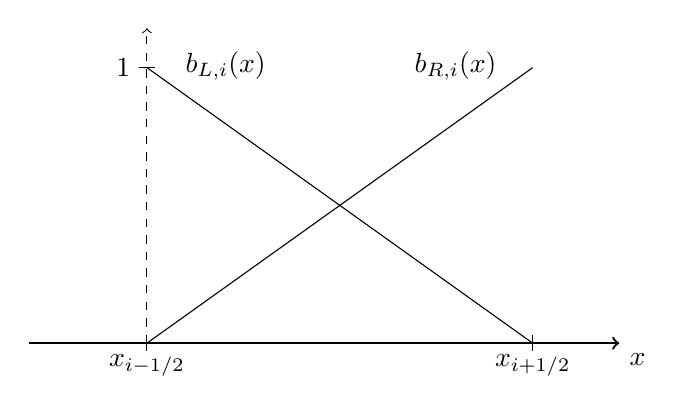
\begin{tikzpicture}[scale=1.0, every node/.style={transform shape}]
            \node at (10.7,4.0) {${1}$  };
            \draw (10.9,4.0) -- (11.1,4.0);
            \draw (11.0,0.4) -- (11.0,0.6) node[below, pos=0.4] {$x_{i-1/2}$};
            \draw (15.90,0.4) -- (15.90,0.6) node[below, pos=0.4] {$x_{i+1/2}$};
            \node at (14.92,4.02) {$b_{R,i}(x)$};
            \node at (12.0,4.02) {$b_{L,i}(x)$};
            \draw [thick,->] (9.5,0.5) -- (17.0,0.5) node[anchor=north west] {$x$};
            \draw [dashed,->] (11.0,0.5) -- (11.0,4.5);
            \draw (11.0,0.5) -- (15.90,4.0);
            \draw (15.90,0.5) -- (11.0,4.0);
        \end{tikzpicture}
    \end{centering}
    \caption{Illustration of linear finite element basis functions $b_{L,i}(x)$ and
    $b_{R,i}(x)$ for spatial element $i$.\label{fig:lin_fe}}
\end{figure}

The spatial moments are defined by integrals weighted with the standard linear finite element (FE)
interpolatory basis functions.  An illustration of the two linear FE basis functions for
the $i$-th element (or cell) is
given in Fig.~\ref{fig:lin_fe}.  The left basis function is defined as
\begin{equation}
    b_{L,i}(x)= \left\{\begin{matrix} \frac{\ds x_\ir - x}{\ds h_i} & x_\il \leq x \leq x_\ir
        \\ 0 &  \text{elsewhere}
    \end{matrix}\right.,
\end{equation}
corresponding to the node $x_\il$.
The right basis function is 
\begin{equation}
    b_{R,i}(x)= \left\{\begin{matrix} \frac{\ds x - x_\il}{\ds h_i} & x_\il \leq x \leq x_\ir
        \\ 0 & \text{elsewhere}
    \end{matrix}\right. ,
\end{equation}
corresponding to the node $x_\ir$. With these definitions, a local linear approximation to a
function $f$ can be formulated as $f(x)\simeq f_{L,i} b_{L,i}(x) + f_{R,i}
b_{R,i}(x),\quad x\in[x_{\il},x_{\ir}]$.\footnote{In literature the linear FE basis functions are
formally defined with support over two adjacent elements.  However, in our notation our 
functions only have non-zero support in element $i$. This accommodates our later
definition of moments and discontinuous unknowns.}

The spatial moments are defined by integrals over the each element, using the two
basis functions.  We use $\mom{\cdot}$ to indicate weighted integration over a
spatial element.  The spatial moments are
\begin{equation}\label{eq:x_moml}
\mom{\cdot}_{L,i} = \frac{2}{h_i} \int_{x_{i-1/2}}^{\xr} b_{L,i}(x) (\cdot) \dd x
\end{equation}
and
\begin{equation}\label{eq:x_momr}
\mom{\cdot}_{R,i} = \frac{2}{h_i} \int_{x_{i-1/2}}^{\xr} b_{R,i}(x) (\cdot) \dd x,
\end{equation}
where the factor of $2/h_i$ is a normalization constant.
In this notation $\mom{\phi}_{L,i}$ and
$\mom{\phi}_{R,i}$ represent spatial moments of the intensity over cell $i$, opposed
to $\phi_{L,i}$ and $\phi_{R,i}$, which represent the interior value of the linear
representation of $\phi(x)$ at $x_\il$ and $x_\ir$ within the cell. 

To simplify notation and discussion, we also define the slope and average moments over a
spatial cell.  The element-averaged scalar intensity is
\begin{equation}
    \phi_i = \frac{1}{h_i} \int_{\xl}^{\xr} \phi(x) \dd x
\end{equation}
and
\begin{equation}
    \phi_{x,i} = \frac{6}{h_i} \int_{\xl}^{\xr} \left(\frac{x-x_i}{h_i} \right)
    \phi(x) \dd x . 
\end{equation}
The linear representation over a cell can be written as $\phi(x) = \phi_i
+ 2\phi_{x,i}(x - x_i)/h_i^2$, for $x\in(\xl,\xr)$. 

\subsection{Definition of Angular Moments}

To reduce the angular dimensionality, positive and
negative half-range integrals of the angular intensity are taken.  The angular integrals
are denoted with a superscript as
\begin{equation}
    (\cdot)^\pm =  \pm\int_0^{\pm1} (\cdot) \dd \mu
\end{equation}
The half-range
integrals of $I$ are defined as $ \phi^+(x) = \int_0^{1} I(x,\mu)\, \dd \mu$ and $
\phi^-(x) =  \int_{-1}^{0} I(x,\mu) \,\dd
\mu$, respectively.  Thus, in terms of half-range quantities, the mean intensity is $\phi = \phi^- +
\phi ^+$.  It is noted that in this notation the flux is defined as
$J=J^-+J^+$, which is not the standard definition for the half-range fluxes, e.g.,
in~\cite{lewis}.

\subsection{Space-Angle Moments of the Radiation Transport Equation}

The LO radiation equations are formed by applying the space and angle moment operators to the
transport equation and performing algebraic manipulation.  We provide a detailed
derivation of the $L$ and $+$ radiation moment equation and state the final results for the
other moment operators.  The independent variables are often suppressed for some, or
all, of the dependent variables for compactness. 

First, the $L$ moment operator is applied to the time-discretized transport equation,
i.e., Eq.~\eqref{eq:trans_td}; application of integration by parts to the streaming term
of the resulting equation yields
\begin{multline}
    -\frac{2}{h_i}\mu I^{n+1}(x_{i-1/2},\mu) + \frac{2}{h_i^2}\int_{\xl}^{\xr} \mu I^{n+1}(x,\mu) \dd x
        +  \left(\sigma_{t,i}^{n+1}+\frac{1}{c \Delta t} \right)  
        \mom{I^{n+1}(x,\mu)}_{L,i} \\ -  \frac{\sigma_{s,i} }{2} \mom{\phi^{n+1}(x)}_{L,i} =
        \frac{1}{2} \mom{\sigma_{a,i}^{n+1} a c T^{n+1,4}(x)}_{L,i} +
  \frac{1}{c\Delta t}\mom{I^n(x,\mu)}_{L,i}.
\end{multline}
Here, the cross sections have been assumed constant over a cell and evaluated with
$T^{n+1}$. Now, the mean
intensity in the scattering term is expanded in terms of half-range unknowns.
The integral can be rewritten in terms of $L$ and $R$ moments by noting that $b_{L,i}(x) +
b_{R,i}(x) = 2/h_i$.  These substitutions are made, independent variables are suppressed, and the resulting equation is
multiplied by $h_i$ to produce
\begin{multline}
    -2\mu I_{i-1/2}^{n+1} + \mom{\mu I^{n+1}}_{L,i} + \mom{\mu I^{n+1}}_{R,i} 
        +  \left(\sigma_{t,i}^{n+1}+\frac{1}{c \Delta t} \right) h_i 
        \mom{I^{n+1}}_{L,i} \\-  \frac{\sigma_{s,i} h_i}{2} \left( \mom{\phi}_{L,i}^{n+1,+} +
  \mom\phi_{L,i}^{n+1,-}\right) = \frac{h_i}{2} \mom{\sigma_a^{n+1} a c T^{n+1,4}}_{L,i} +
  \frac{h_i}{c\Delta t}\mom{I^n}_{L,i},
\end{multline}
where $I_{i-1/2}(\mu)\equiv I(x_{i-1/2},\mu)$.
The resulting equation is integrated over the positive half range:
\begin{multline}\label{eq:spat_mom}
    -2\left({\mu} I_{i-1/2}^{n+1}\right)^+ + \mom{\mu I^{n+1}}^+_{L,i} + \mom{\mu
        I^{n+1}}^+_{R,i} 
        +  \left(\sigma_{t,i}^{n+1}+\frac{1}{c \Delta t} \right) h_i 
  \mom{\phi}_{L,i}^{n+1,+} \\-  \frac{\sigma_{s,i} h_i}{2} \left( \mom{\phi}_{L,i}^{n+1,+} +
  \mom\phi_{L,i}^{n+1,-}\right) = \frac{h_i}{2} \mom{\sigma_a^{n+1} a c T^{n+1,4}}_{L,i} +
  \frac{h_i}{c\Delta t}\mom{\phi}_{L,i}^{n,+}.
\end{multline}

\subsection{The Angular Consistency Terms}
\label{sec:ang_cons}

Now, algebraic manipulations are performed on the streaming terms to produce face and
volume averages of $\mu$, weighted by the intensity.  Each term in the streaming
term of Eq.~\eqref{eq:spat_mom} is multiplied by a factor of unity, with the desired unknown appropriate to each term
in the numerator and denominator, as in~\cite{wolters}.  Temporarily dropping the time
index for clarity, the manipulations applied to
the streaming term are as follows:
    \begin{align} \label{eq:line1}
        {\displaystyle \left \langle \mu \pderiv{I}{x} \right \rangle_L^+ } & = 
        -\frac{\ds2}{\ds h_i} \left(\mu I_{i-1/2}\right)^+ + \frac{\ds 1}{\ds h_i}\left[
    \mom{\mu I}_{L,i}^+ + \mom{\mu I}_{R,i}^+ \right] \\
        & =  
        -\frac{\ds2}{\ds h_i} \left(\mu I_{i-1/2}\right)^+
        \! \frac{\ds(I_{i-1/2})^+}{\ds(I_{i-1/2})^+}  \;    + \frac{\ds 1}{\ds h_i}\left[ \;
        \mom{\mu I}_{L,i}^+ \! \frac{\ds\mom{I}_{L,i}^+}{\ds\mom{I}_{L,i}^+} \; + \; \mom{\mu
        I}_{R,i}^+ \! \frac{\ds\mom{I}_{R,i}^+}{\ds\mom{I}_{R,i}^+} \right] \\
        & =  -\frac{\ds2}{\ds h_i} \left\{ {\frac{\ds \left( \mu I
            \right)^+_{i-1/2} }{\ds\phi^+_{i-1/2}}} \right\}
            \phi^+_{i-1/2} + \frac{\ds 1}{\ds h_i} \left[ \left\{ {\frac{\ds\mom{\mu
        I}_{L,i}^+}{\ds\mom{\phi}_{L,i}^+}} \right \} \mom{\phi}_{L,i}^+  +
        \left\{ {\frac{\ds\mom{\mu I}_{R,i}^+}{\ds\mom{\phi}_{R,i}^+}} \right\}
    \mom{\phi}_{R,i}^+ \right]
    \end{align}
The ratios in braces are what we will formally define as \emph{angular consistency terms}.
These nonlinear functionals are approximated by the HO solver, similar to the approach
in~\cite{wolters}.  The angular consistency
term for the $L$ and $+$ moments is defined as
\begin{equation}\label{eq:ang_cons_vol}
    \cur{{\mu}}_{L,i}^{n+1,+} \equiv \frac{\mom{\mu I^{n+1}}_{L,i}^+}{\mom{I^{n+1}}_{L,i}^+} =  \frac{
{\displaystyle \frac{2}{h_i}} \int\limits_0^1 \int\limits_\xl^\xr \mu \, b_{L,i}(x)
I^{n+1}(x,\mu) \dd x \dd \mu } 
{{\displaystyle \frac{2}{h_i}} \int\limits_0^1 \int\limits_\xl^\xr \, b_{L,i}(x)
I^{n+1}(x,\mu) \dd x \dd \mu } .
\end{equation}
The consistency terms on the face represent averaging at a point, with a similar
definition as
\begin{equation}\label{eq:ang_cons_face}
    {\mu}_{i+1/2}^{+} \equiv \frac{\left(\mu I_{i+ 1/2}\right)^+}{\phi_{i+1/2}^+}=  \frac{
        {\displaystyle \int\limits_0^1 \mu I(x_{i+1/2},\mu) \dd \mu }} 
        {{\displaystyle \int\limits_0^1 I(x_{i+1/2},\mu) \dd \mu }} \;.
\end{equation}
There are analogous definitions for the $R$ and $-$ moments, e.g.,
\begin{equation}\label{eq:ang_cons_vol}
    \cur{{\mu}}_{R,i}^{n+1,-} \equiv \frac{\mom{\mu I^{n+1}}_{R,i}^-}{\mom{I^{n+1}}_{R,i}^-} =  \frac{
        {\displaystyle \frac{2}{h_i}} \int\limits_{-1}^0 \int\limits_\xl^\xr \mu \, b_{R,i}(x)
I^{n+1}(x,\mu) \dd x \dd \mu } 
{{\displaystyle \frac{2}{h_i}} \int\limits_{-1}^0 \int\limits_\xl^\xr \, b_{R,i}(x)
I^{n+1}(x,\mu) \dd x \dd \mu } .
\end{equation}
Substitution of Eq.~\eqref{eq:ang_cons_vol}~and~\eqref{eq:ang_cons_vol} simplifies
moments of the streaming
term for the $L$ and $+$ operators:
\begin{equation}\label{eq:stream_mom}
        {\displaystyle \left \langle \mu \pderiv{I}{x} \right \rangle_L^+ } = 
        -\frac{\ds2}{\ds h_i} \mu_{i-1/2}^+ I_{i-1/2}^+ + \frac{1}{h_i}\left[
        \cur{\mu}_{L,i}^+ \mom{\phi}^+_{L,i} + \cur{\mu}_{R,i}^+ \mom{\phi}_{R,i}^+
    \right]
\end{equation}
It is noted that this expression does not contain a cross section in the denominator,
such as in the variable Eddington factor approach~\cite{ferguson}, eliminating 
issues in a void where $\sigma_t=0$.


\subsection{The Exact Radiation Moment Equations}

A final form of the moment equation resulting from application of the $L$ moment and
positive half-range integral is obtained by substitution of 
Eq.~\eqref{eq:stream_mom} into Eq.~\eqref{eq:spat_mom}:
\begin{multline}\label{eq:exact_lmomp}
    -2{\mu}_{i-1/2}^{n+1,+} \phi_{i-1/2}^{n+1,+} + \cur {\mu}_{L,i}^{n+1,+}
  \mom{\phi}_{L,i}^{n+1,+}
  +  \cur\mu_{R,i}^{n+1,+}
  \mom{\phi}_{R,i}^{n+1,+} +  \left(\sigma_{t,i}^{n+1}+\frac{1}{c \Delta t} \right) h_i 
  \mom{\phi}_{L,i}^{n+1,+} \\-  \frac{\sigma_{s,i} h_i}{2} \left( \mom{\phi}_{L,i}^{n+1,+} +
  \mom\phi_{L,i}^{n+1,-}\right) = \frac{h_i}{2} \mom{\sigma_a^{n+1} a c T^{n+1,4}}_{L,i} +
  \frac{h_i}{c\Delta t}\mom{\phi}_{L,i}^{n,+},
\end{multline}
The other radiation moment equations are derived analogously.  
Pairwise application of the $L$ and $R$ basis
moments with the $+$ and $-$ half-range integrals to Eq.~\eqref{eq:trans_td} 
ultimately yields four moment
equations per cell.  The equation for the $R$ and $+$ moment is
\begin{multline}\label{eq:exact_rmomp}
    2{\mu}_{i+1/2}^{n+1,+} \phi_{i+1/2}^{n+1,+} - \cur {\mu}_{L,i}^{n+1,+}
  \mom{\phi}_{L,i}^{n+1,+}
  -  \cur\mu_{R,i}^{n+1,+}
  \mom{\phi}_{R,i}^{n+1,+} +  \left(\sigma_{t,i}^{n+1}+\frac{1}{c \Delta t} \right) h_i 
  \mom{\phi}_{R,i}^{n+1,+} \\-  \frac{\sigma_{s,i} h_i}{2} \left( \mom{\phi}_{R,i}^{n+1,+} +
  \mom\phi_{R,i}^{n+1,-}\right) = \frac{h_i}{2} \mom{\sigma_a^{n+1} a c T^{n+1,4}}_{R,i} +
  \frac{h_i}{c\Delta t}\mom{\phi}_{R,i}^{n,+},
\end{multline}
The equations for the negative half-range moment are identical to the above with the
negative half-range integrals replacing the positive where applicable.  Explicitly,
\begin{multline}\label{eq:exact_lmomm}
    -2{\mu}_{i-1/2}^{n+1,-} \phi_{i-1/2}^{n+1,-} + \cur {\mu}_{L,i}^{n+1,-}
  \mom{\phi}_{L,i}^{n+1,-}
  +  \cur\mu_{R,i}^{n+1,-}
  \mom{\phi}_{R,i}^{n+1,-} +  \left(\sigma_{t,i}^{n+1}+\frac{1}{c \Delta t} \right) h_i 
  \mom{\phi}_{L,i}^{n+1,-} \\-  \frac{\sigma_{s,i} h_i}{2} \left( \mom{\phi}_{L,i}^{n+1,+} +
  \mom\phi_{L,i}^{n+1,-}\right) = \frac{h_i}{2} \mom{\sigma_a^{n+1} a c T^{n+1,4}}_{L,i} +
  \frac{h_i}{c\Delta t}\mom{\phi}_{L,i}^{n,-}
\end{multline}
and
\begin{multline}\label{eq:exact_rmomm}
    2{\mu}_{i+1/2}^{n+1,-} \phi_{i+1/2}^{n+1,-} - \cur {\mu}_{L,i}^{n+1,-}
  \mom{\phi}_{L,i}^{n+1,-}
  -  \cur\mu_{R,i}^{n+1,-}
  \mom{\phi}_{R,i}^{n+1,-} +  \left(\sigma_{t,i}^{n+1}+\frac{1}{c \Delta t} \right) h_i 
  \mom{\phi}_{R,i}^{n+1,-} \\-  \frac{\sigma_{s,i} h_i}{2} \left( \mom{\phi}_{R,i}^{n+1,+} +
  \mom\phi_{R,i}^{n+1,-}\right) = \frac{h_i}{2} \mom{\sigma_a^{n+1} a c T^{n+1,4}}_{R,i} +
  \frac{h_i}{c\Delta t}\mom{\phi}_{R,i}^{n,-},
\end{multline}
Ultimately, the two half-ranges will be treated differently when the equations are closed
spatially.

\subsection{Material Energy Equations}

To derive the LO material energy equations, an approximation must be introduced to relate
$T(x)$ and $T^4(x)$ within a cell.  We represent $T(x)$ spatially 
with a LDFE trial space, i.e., $ T(x) \simeq T_{L,i} b_{L,i}(x) + T_{R,i} b_{R,i}(x),\quad x\in(x_{i-1/2},x_\ir)$.
This trial space will ensure preservation of the equilibrium
diffusion limit and limit artificial propagation of energy across the system~\cite{teleportation}. 
Similarly, the emission term is represented in the material and radiation equations with the LDFE
interpolant $T^4(x)\simeq T_{L,i}^4 b_{L,i}(x) + T_{R,i}^4 b_{R,i}(x)$.   The $L$ and $R$ spatial moments are taken of the material
energy equations, and the LDFE representations for $T(x)$ and $\sigma_a a c T^4(x)$ are used to
simplify the spatial integrals. The final LO material energy
 equation resulting from application of the $L$ moment is
 \begin{multline}\label{eq:lo_mat_dis1}
     \frac{\rho_i c_{v,i}}{\Delta t}\left[ \left(\frac{2}{3}T_{L,i} + \frac{1}{3}T_{R,i}
        \right)^{n+1} - \left(\frac{2}{3}T_{L,i} + \frac{1}{3}T_{R,i}
    \right)^{n} \right]  + \sigma_{a,i}^{n+1} \left( \mom{\phi}_{L,i}^+ +
    \mom{\phi}_{L,i}^- \right)^{n+1} \\ = \sigma_{a,i}^{n+1}a c
\left( \frac{2}{3} T_{L,i}^4 + \frac{1}{3}T_{R,i}^4
        \right)^{n+1}.
\end{multline}
The equation for the $R$ moment is
 \begin{multline}\label{eq:lo_mat_dis2}
     \frac{\rho_i c_{v,i}}{\Delta t}\left[ \left(\frac{1}{3}T_{L,i} + \frac{2}{3}T_{R,i}
        \right)^{n+1} - \left(\frac{1}{3}T_{L,i} + \frac{2}{3}T_{R,i}
    \right)^{n} \right]  + \sigma_{a,i}^{n+1} \left( \mom{\phi}_{R,i}^+ +
    \mom{\phi}_{R,i}^- \right)^{n+1} \\ = \sigma_{a,i}^{n+1}a c
\left( \frac{1}{3} T_{L,i}^4 + \frac{2}{3}T_{R,i}^4
        \right)^{n+1}.
\end{multline}
Cross sections have been assumed constant over each element, evaluated at the
average temperature within the element, i.e., $\sigma_{a,i}^{n+1} =
\sigma_{a,i}([T^{n+1}_{L,i}+T^{n+1}_{R,i}]/2)$.
Because the material energy balance equation
 only contains angularly integrated quantities, there is no need to take angular
 moments of the above equations.  


\section{Closing the LO Equations in Space and Angle}
\label{sec:closure}

At this point, the LO equations have too many unknowns: the relation between the volume
and face averaged quantities and the angular consistency parameters are not known a
priori. The HO solution is used to eliminate the consistency parameters and other
approximations are used to eliminate the extra spatial unkonwns from the equations.
The six degrees of freedom (DOF) over each cell $i$ are the four moments $\mom{\phi}_{L,i}^+$,
$\mom{\phi}_{R,i}^+$, $\mom{\phi}_{L,i}^-$, and $\mom{\phi}_{R,i}^-$ and the two
spatial edge values $T_{L,i}$ and $T_{R,i}$.  After closure, the four radiation and two material
energy equations define a system of equations for the six DOF, coupled spatially through
the streaming term.  

Before introducing the additional closures, we emphasize that at this point the only spatial or
angular approximations to the radiation  moment equations are an LDFE
representation for $T^4(x)$ and cell-averaged cross sections; these moment equations are exact with
respect to the chosen time discretization and these approximations.  The material energy
equations, as well as the emission source, required an approximation of LDFE in space for $T(x)$ and $T^4(x)$.  Some
approximation is always necessary
to relate $T$ and $T^4$.

\subsection{Angular Closure}

The angular consistency
parameters (e.g., Eq.~\eqref{eq:ang_cons_vol} and~\eqref{eq:ang_cons_face}) are not known a priori. 
A lagged estimate of $I^{n+1}$ from the previous HO solve is
used to estimate the angular consistency parameters. In the HOLO algorithm, the equations for LO unknowns at iteration $k+1$ use consistency parameters
computed using the latest HO solution $\tilde{I}^{n+1,k+1/2}$
as an approximation for $I^{n+1}(x,\mu)$, e.g.,
\begin{equation}\label{eq:ang_cons_vol}
    \cur{{\mu}}_{L,i}^{n+1,+} \simeq \frac{\mom{\mu
    \tilde I_{HO}^{n+1,k+1/2}}_{L,i}^+}{\ds \mom{\tilde I_{HO}^{n+1,k+1/2}}_{L,i}^+} =
    \frac{\ds 
{\displaystyle \frac{2}{h_i}} \int\limits_0^1 \!\int\limits_\xl^\xr \mu \, b_{L,i}(x)
\tilde I^{n+1,k+1/2}_{HO}(x,\mu)\, \dd x \dd \mu } 
{\ds {\displaystyle \frac{2}{h_i}} \int\limits_0^1 \!\int\limits_\xl^\xr  b_{L,i}(x)
\tilde I^{n+1,k+1/2}_{HO}(x,\mu)\, \dd x \dd \mu } .
\end{equation}
We evaluate these terms using quadrature based
on the LDFE functional representation $\tilde I_{HO}(x,\mu)$ provided by the HO solution.

\subsection{LDFE Spatial Closure}

After approximating the angular consistency terms in the time-discretized LO moment equations, 
a equation relating the spatial moments and outflow face values is
needed to eliminate the final auxiliary unknowns, i.e., a spatial closure.
We will eliminate the face terms to produce equations exclusively the desired moment
unknowns.  Several closures were investigated.  The simplest closure
is a linear-discontinuous (LD) spatial closure with the usual upwinding
approximation~\cite{morel_ldtrt}.  A closure based on the HO solution is discussed in
Sec.~\ref{sec:spat_clos}.  Because there are no derivatives of $T$ in Eq.~\eqref{eq:mat_td}, there is no need
to define $T$ on the faces in Eq.~\eqref{eq:lo_mat_dis1} and Eq.~\eqref{eq:lo_mat_dis2};
only moments of $\phi$ appear in the material energy
equations, thus they are fully defined at this point and require no additional spatial
closure.  

Now, the LDFE closure is applied to the radiation moment equations for the case of
positive flow (i.e., Eq.~\eqref{eq:exact_lmomp} and~\eqref{eq:exact_rmomp}). The LD
closure over for the $i$-th cell and positive $\mu$ 
is illustrated in Fig.~\ref{fig:ld_il}.  The face terms $\mu_{i-1/2}$ and $\phi_{i-1/2}$
are upwinded from the previous cell $i-1$ or from a boundary condition; the terms
at $x_{i+1/2}$ are linearly extrapolated, computed using the $L$ and $R$ basis
moments.  The linear approximation $\phi^+(x)=b_{L,i}(x)\phi^+_{L,i} +
b_{R,i}(x)\phi^+_{R,i}$, for $x\in(\xl,\xr]$, is substituted into the definition for
the moments (i.e., Eq.~\eqref{eq:x_moml}~and~\eqref{eq:x_momr}) and solved for the LD edge value
$\phi_{i,R}^+$; The resulting outflow relation for positive flow is $\phi^+_{i+1/2} \equiv \phi_{i,R}^+ = 2\mom{\phi}_{R,i}^+ -
\mom{\phi}_{L,i}^+$; the LD closure for the negative half range produces $\phi^-_{i-1/2} = 2\mom{\phi}_{L,i}^- -
\mom{\phi}_{R,i}^+$. The $L$ moment and positive half-range equation with the LD closure and upwinding is
\begin{multline} 
    -2{\mu}_{i-1/2}^{n+1,+} \left(2\mom{\phi}_{R,i-1}^{n+1,+} -   \mom{\phi}_{L,i-1}^{n+1,+}      \right) + \cur {\mu}_{L,i}^{n+1,+}
  \mom{\phi}_{L,i}^{n+1,+}
  +  \cur\mu_{R,i}^{n+1,+}
  \mom{\phi}_{R,i}^{n+1,+}\\ +  \left(\sigma_{t,i}^{n+1}+\frac{1}{c \Delta t} \right) h_i 
  \mom{\phi}_{L,i}^{n+1,+} -  \frac{\sigma_{s,i} h_i}{2} \left( \mom{\phi}_{L,i}^{n+1,+} +
  \mom\phi_{L,i}^{n+1,-}\right)\\  = \frac{h_i}{2} \mom{\sigma_a^{n+1} a c T^{n+1,4}}_{L,i} +
  \frac{h_i}{c\Delta t}\mom{\phi}_{L,i}^{n,+}.
\end{multline}
Similar equations can be derived for the other directions and moments, fully defining the radiation
equations.   The closed equations are equivalent in numerical complexity to an LDFE
discretization of the S$_2$ equations~\cite{morel_ldtrt,lewis}, but with different quadrature points on the face
and interior.

\begin{figure}[H]
    \centering
    {\resizebox{0.5\textwidth}{!}{
        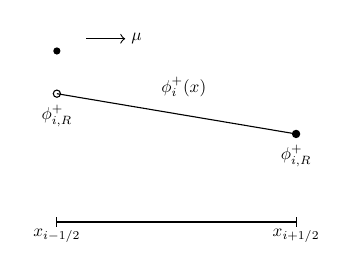
\begin{tikzpicture}[scale=0.62, every node/.style={transform shape}]
            \draw (1.0,4.0) node[fill,circle,inner sep=0pt,minimum
            size=4.2pt] {};
            \draw [->] (1.6,4.25) -- (2.4,4.25) node[anchor=west] {$\mu$};
            \draw (1.0,0.4) -- (1.0,0.6) node[below, pos=0.4] {$x_{i-1/2}$};
            \draw (5.90,0.4) -- (5.90,0.6) node[below, pos=0.4] {$x_{i+1/2}$};
            \node at (3.6,3.26) {$\phi_i^+(x)$};
            \node[anchor=north] at (5.9,2.2) {${\phi^+_{i,R}}$};
            \draw [thick] (1.0,0.5) -- (5.9,0.5) node[anchor=north west] {};
            \filldraw[color=black, fill=white] (1,3.1250) circle (2.1pt);
            \draw (1.0,3.125) -- (5.90,2.30);
            \node[anchor=north] at (1.0,3.025) {${\phi^+_{i,R}}$};
            \filldraw (5.9,2.30) circle (2.1pt);
        \end{tikzpicture}
    }}
    \caption{Linear discontinuous trial space for half-range mean intensity and $\mu>0$,
        in LO equations.\label{fig:ld_il}}
\end{figure}

Note that we have chosen to leave $\mu_{i-1/2}^{n+1,+}$ as a value to be estimated from the HO solver,
which is more conducive to the HO spatial closures described in
Sec.~\ref{sec:spat_clos}.
Alternatively, the spatial closure could be introduced before performing the algebraic
manipulation to form consistency terms (e.g., into Eq.~\eqref{eq:line1}).  This would produce only volume-weighted consistency
terms in the equations.  




\subsection{Boundary Conditions}

For all spatial closures, the specified incident angular intensity is
incorporated into the upwinding term of the appropriate radiation moment equation.   At the left
boundary, the upwinded current is known, so for that $L$ moment equation
\begin{equation}
    \mu_{1/2}^+ \phi_{1/2}^+ = \int_{0}^1 \mu I^{inc,+}(\mu) \dd \mu,
\end{equation}
where $I^{inc,+}(\mu)$ is the specified incident angular intensity at the left boundary.  For all
results in this work, only isotropic incident intensities were considered.
A similar expression is derived for the right boundary.
  For S$_2$-equivalent LO solves, i.e., all consistency
terms are $\pm 1/\sqrt{3}$, the half-range flux in the above equation is renormalized by
multiplying the term in the moment equations by $2/\sqrt{3}$ to produce accurate solutions~\cite{morel_notes}.     


\section{Newton's Method for LO Equations}
\label{sec:newton_overview}

Summation over all cells of the closed equations forms a global system of coupled equations.
The equations are nonlinear due to the Planckian emission source.  
We have used a local Newton's method to solve the nonlinear system, based on a standard linearization of the Planckian source with cross
sections evaluated at temperatures from the previous iteration, as described
in~\cite{morel_ldtrt}.  A derivation of the LO Newton equations is given
in~\ref{app:lo_newton}.

The equations for each half-range are coupled together via scattering.  
In one spatial dimension, the scattering terms can be included in the discrete system
matrix and directly inverted.  We consider an alternative iterative solution method that
could be more easily extended to higher spatial dimensions in Chapter~\ref{chp:dsa}.
For the direct solution method, isotropic scattering,
including effective scattering terms from the linearization, are included in the system matrix. The system
matrix is an asymmetric, banded matrix with a band width of seven and is inverted
directly. 
Newton iterations are repeated until $\phi^{n+1}(x)$ and $T^{n+1}(x)$ are converged
to a desired relative tolerance.  Convergence in the Newton iterations is calculated using the spatial $L_2$
norm of the change in $\phi^{n+1}(x)$ and $T^{n+1}(x)$, relative to the norm of each
solution.  

In certain problems, the nonlinearities of the system can lead to divergence of the Newton
iterations.  This is often the result of taking relatively large time steps for problems with large
values of $\sigma_a$ and small values of $\rho c_v$.  To prevent divergence, a damped
Newton method~\cite{damped_newton} can be used, at the cost of increased numbers of iterations.  For a
damped Newton's method, the estimated change in the solution between iterations is multiplied by a factor $\xi\in(0,1)$, where $\xi$ is referred to as the damping factor.
Sufficient reduction of the change in solutions between iterations will allow iterations
to continue converging, by ensuring the solution remains with the domain of convergence.  
The details of modifying the Newton iterations in this work to include a damping factor are given in
App.~\ref{app:damped_newton}.  For simplicity, a fixed value of $\xi$ was used for all
iterations in problems where damping was found to be necessary.

%Application of the first order Taylor expansion in time of the
%gray emission source, about some temperature $T^*$ at some
%time near $t^{n+1}$ gives
%\begin{equation}\label{new_planck}
%    \sigma_a^* a c T^{4,n+1} \simeq \sigma_a^* a c \left[T^{*4} + (T^{n+1} - T^*) 4T^{*3} \right]
%\end{equation}
%where the superscript $*$ denotes evaluation at $T^*$. A spatially discretized form
%of this expression is substituted
%into the emission term in the discretized material
%energy equations, e.g., Eq.~\eqref{lo_mat_dis}.  This allows for the material energy
%equation to be eliminated from the system, introducing effective scattering and
%emission sources into the right hand side
%of the LO radiation equations. This defines four linear equations for the four remaining radiation unknowns. 
%Once these linear equations have been solved for $\phi^{n+1}$, a new estimate of
%$T^{n+1}$ can be determined using the same linearization (Eq.~\eqref{new_planck}) to
%conserve the total energy.  This estimate of $T^{n+1}$ can now be used as $T^*$ to form a more
%accurate linearization of the emission source. 


\section{Accuracy of LO Equations in the Equilibrium Diffusion Limit}
\label{sec:edl_overview}

In our LO scheme, the
LO equations use an LDFE representation for the temperature.  The radiation terms can also
be closed with an LDFE closure.  In the EDL limit, the MC HO
solution will estimate angular consistency terms associated with an isotropic intensity,
based on a spatially LD emission source.  This produces LO equations that are equivalent to
the S$_2$ equations, but with quadrature points defined by $\pm 1/2$.  Because the spatial closure produces equations that are equivalent to an LDFE
solution to the S$_2$ equations, we expect the equations to preserve the equilibrium diffusion
limit; the LDFE discretization of the S$_2$ equations is known to preserve the EDL based on discrete asymptotic analysis~\cite{morel_ldtrt}.

\section{Fix-ups for Negative Solutions with LDFE Closure}
\label{sec:ldfe_fixups}

The linear-discontinuous (LD) closure with upwinding is not strictly positive.  In particular, for
optically thick cells with a steep intensity gradient, the linear representations for
$\phi(x)$ and $T(x)$ can go below the floor temperature or negative. 
The floor temperature $T_{\min}$ is defined as the initial
temperature of the material and radiation in problems where boundary sources are
applied at each of the boundaries.  In such problems the radiation and material should
continue to heat on the interior of the domain, and physically should not fall below
the initial temperature. 
Negative values of intensity can propagate to adjacent cells. In thick regions of
TRT problems, reasonably fine spatial cells can still be on the order of millions of mean
free paths; negative values with an LD representation are unavoidable in practice for
such cells and mesh refinement is of minimal use. 

Typically, for a standard LDFE Galerkin spatial discretization,
the equations are lumped to produce a discretization that is strongly resistant to
negative values (for 1D)~\cite{morel_ldtrt}.
However, standard FE lumping
procedures would introduce difficulties in computing the consistency terms from the
HO solution.  
 Alternatively, we have derived a modified spatial closure that produces
unknowns equivalent to those from a lumped LD method in 1D.
The $L$ and $R$ moments are defined the same as before,
preserving the average within a cell, but the relation between the moments and
the outflow is modified. 
In the lumping-equivalent closure, the outflows are defined as
\begin{align}
    \phi_{i+1/2}^+ &= \mom{\phi}_{i,R}^+ \\
    \phi_{i-1/2}^- &= \mom{\phi}_{i,L}^-. 
\end{align}
The system is then fully defined with upwinding and the assumption of a linear relationship on
interior of the element.  This modified closure produces a linear
representation that preserves zeroth moment, but the relation between the slope of the line and the 
first spatial moment has been modified.  Because the basis functions $b_{R,i}(x)$ and $b_{L,i}(x)$ are strictly
positive, the outflows tends to be positive. Strong sources and gradients can still lead to
negativities at the edges of the LD representation.  Details on the
derivation of this relation are in Appendix~\ref{app:lo_mom_relations}. 
The lumping closure was optionally applied in all cells or only in cells where negative
 intensities occur.  

For simplicity,
we also lump the emission source and temperature terms in the equations following the
standard procedure~\cite{morel_ldtrt}.  For example, the lumped version of Eq.~\eqref{eq:lo_mat_dis1}
is
\begin{equation}\label{eq:lumped_mat}
     \frac{\rho_i c_{v,i}}{\Delta t}\left(T_{L,i}^{n+1} - T_{L,i}^{n}\right)  + \sigma_{a,i}^{n+1} \left( \mom{\phi}_{L,i}^+ +
    \mom{\phi}_{L,i}^- \right)^{n+1} \\ = \sigma_{a,i}^{n+1}a c
    \left( T_{L,i}^{n+1}\right)^4
    \end{equation}
noting that no modification was made to the radiation moment term in this equation.  It was found that
lumping the temperature equations generally produced more robustness than exclusively
modifying the spatial closure, but it is not necessary for all problems.

\subsection{Balance Preserving Fixup}

We also investigated an alternative closure of the equations based on energy conservation
and forcing the appropriate edge value to be the floor value.
The equations within cells that produce a negativity are modified to ensure the edge
intensities are not below the floor temperature, and energy balance is
conserved.  This fixup is applied in cells where a negative intensity is detected during
a Newton iteration.  For example, if $\phi^+_{R,i}$
is found to be negative, the modified equations (for the positive half range) in that cell are
the balance equation, i.e., 
\begin{multline}\label{eq:floor_outflow}
    -{\mu}_{i-1/2}^{n+1,+} \left(2\mom{\phi}_{R,i-1}^{n+1,+} -   \mom{\phi}_{L,i-1}^{n+1,+}      \right) +
    {\mu}_{i+1/2}^{n+1,+} \left(2\mom{\phi}_{R,i}^{n+1,+} -
    \mom{\phi}_{R,i}^{n+1,+}\right) \\       
   +  \left(\sigma_{t,i}^{n+1}+\frac{1}{c \Delta t} \right)
  \frac{h_i}{2} \left(\mom{\phi}_{L,i}^{n+1,+} + \mom{\phi}_{R,i}^{n+1,+}\right) -  \frac{\sigma_{s,i} h_i}{4} \left( \mom{\phi}_{L,i}^{n+1} +
  \mom\phi_{R,i}^{n+1}\right)\\  = \frac{h_i}{4} \sigma_{a,i}^{n+1} a c \left(
    \mom{T^{n+1,4}}_{L,i} + \mom{T^{n+1,4}}_{R,i} \right) +
  \frac{h_i}{2c\Delta t}\left(\mom{\phi}_{L,i}^{n,+} + \mom{\phi}_{R,i}^{n,+}\right)
\end{multline}
and the closure equation, i.e., 
\begin{equation}\label{eq:clos_outflow}
    2\mom{\phi}_{i,R}^+ - \mom{\phi}_{i,L}^+ = T_{\min}.
\end{equation}

Because our solution method directly inverts the LO system,
negative edge intensities must be detected, the fix-up applied locally to all elements and half-ranges
where necessary, and then that Newton solve
repeated.  In practice, this flooring procedure was observed to produce positive answers,
but was not as robust as the lumping closure in all cells.  In general, as the time step
size or problem nonlinearities were increased, this fixup led to the Newton
solves diverging.  




\section{Spatial Closure based on the HO Solution}
\label{sec:spat_clos}

This sections describes an alternative spatial closure to the LO equations based on 
a parametric relation from the HO solution. In addition to estimating the angular
consistency terms, the HO intensity estimates a relation between volume and face-averaged
intensities to eliminate the remaining unknowns from the equations.  In the remainder of
this section, we will motivate the HO spatial closure by manipulating a half-range balance
equations to form a single unknown for each cell and half range.  We will then discuss
the forms of HO spatial closures investigated, based on modifications to standard spatial closures.

\subsection{Motivation}

A half-range balance equation for $\mu>0$ is formed by adding the
exact $L$ and
$R$ radiation moment equations given by
Eq.~\eqref{eq:exact_lmomp}~and~\eqref{eq:exact_rmomp}, i.e.,
\begin{equation}\label{eq:hr_bal}
    \mu^+_{i+1/2}\phi_{i+1/2}^+ - \mu^+_{i-1/2}\phi_{i-1/2}^+ +
    {\sigma_{a,i}h_i} \phi_i^+ = \frac{h_i}{2} q_i,
\end{equation}
where $q_i$ represents the cell-averaged emission source.  In the HOLO algorithm, after
estimating the consistency terms $\mu_{i\pm1/2}^+$ upwinding the inflow term
$\phi_{i-1/2}^+$, an additional equation is needed to eliminate the outflow $\phi_{i+1/2}^+$ to produce an
equation for a single unknown $\phi_{i}^+$.  Standard spatial discretizations techniques
use a fixed approximation for all cells to eliminate the outflow in terms of other
unknowns.  Alternatively, the HO solution can be used to estimate a parametric relation
between the other unknowns and the outflow, i.e.,
\begin{equation}\label{eq:ho_clos}
    \phi_{i+1/2}^+ = f(\gamma^{+,HO}_i, \phi_i^+, \phi_{x,i}^+, \phi_{i-1/2}^+),
\end{equation}
where $\gamma^{HO,+}_i$ is a local constant to be estimated with the HO solution and $f$ is some
function of some number of the input
variables.  The ECMC solution can provide all of the unknowns in the above equation, so
the value of $\gamma^{HO}_i$ can be determined directly. 

If the problem were linear, or the nonlinear problem was fully converged,
then application of this closure can ensure that the HO and LO equations produce the same
moments, preserving the HO accuracy.  To produce the
same moments, the HO solution must also satisfy the local balance equation, e.g.,
Eq.~\eqref{eq:hr_bal}.  Then the LO equations and HO equations must have the same moments
to satisfy both Eq.~\eqref{eq:ho_clos} and Eq.~\eqref{eq:hr_bal}, upon nonlinear
convergence of the outer HOLO iterations. If any higher moments are introduced through the spatial closure,
then the HO solution must also satisfy the corresponding balance equations that the LO
equations do.  For example, both the LO and HO equation must satisfy the
first moment equation in space if the closure is a function of the first moment.  

As TRT problems are non-linear (i.e., scattering or thermal emission are included in
$q$), the moments will only be preserved upon non-linear convergence of the source.  The
nonlinearity introduces the possibility for stability
issues, particularly with MC noise.  However, we have already consistently formed angular consistency terms, so the
the spatial closure should be more stable than introducing other terms, such as
in NDA methods~\cite{rmc,willert}. 





\subsection{Choice of Spatial Closure}
\label{sec:spat_clos_options}

We will
explore two different closure relations based on modifications to the standard LD closure: a scaled slope, i.e.,
\begin{equation}\label{eq:cl_slope1}
    \phi_{i\pm1/2}^\pm = \phi_i^+ \pm \gamma_i^{\pm} \phi_{x,i}^+
\end{equation}
and a scaled average
\begin{equation}\label{eq:cl_avg1}
    \phi_{i\pm1/2}^\pm = \gamma_i^{\pm} \phi_i^+ \pm \phi_{x,i}^+,
\end{equation}
where a value of $\gamma_i = 1$ produces the standard linear discontinuous expressions for
the extrapolated outflows.  Our LO system is formulated in terms of $L$ and $R$ moments, rather than the average and
slope.  Thus, Eq.~\eqref{eq:cl_slope1} and~\eqref{eq:cl_avg1} are expressed in terms of the $L$ and $R$
unknowns, using the relations given in App.~\ref{app:lo_mom_relations}.  In terms of these
moments, the scaled-slope closure is
\begin{align}\label{eq:cl_slope}
    \phi_{i+1/2}^+  &= \left(\frac{\ds 1 - 3 \gamma_i^+}{\ds 2 }  \right)
    \mom{\phi}_{L,i}^+ + \left(\frac{\ds 1 + 3 \gamma_i^+}{\ds 2 }  \right)
    \mom{\phi}_{R,i}^+ \\
    \phi_{i-1/2}^-  &= \left(\frac{\ds 1 + 3 \gamma_i^-}{\ds 2 }  \right)
    \mom{\phi}_{L,i}^- + \left(\frac{\ds 1 - 3 \gamma_i^-}{\ds 2 }  \right)
    \mom{\phi}_{R,i}^- 
\end{align}
and the scaled-average relation is
\begin{align}\label{eq:cl_avg}
    \phi_{i+1/2}^+  &= \left(\frac{\ds  \gamma_i^+ - 3}{\ds 2 }  \right)
    \mom{\phi}_{L,i}^+ + \left(\frac{\ds \gamma_i^+ + 3}{\ds 2 }  \right)
    \mom{\phi}_{R,i}^+ \\
    \phi_{i-1/2}^-  &= \left(\frac{\ds \gamma_i^- + 3}{\ds 2 }  \right)
    \mom{\phi}_{L,i}^- + \left(\frac{\ds \gamma_i^- - 3}{\ds 2 }  \right)
    \mom{\phi}_{R,i}^- .
\end{align}

The HO solution is used to estimate $\gamma_i$. The MC solution must be modified
to tally the MC estimated intensity on faces. For example, for $\mu>0$, the LO equations for
moments at $k+1$ use closure parameters evaluated at $k+1/2$ as
\begin{equation}
    \gamma_i^{+,HO,k+1/2} = \frac{\phi_{i+1/2}^{+,HO,k+1/2} -
    \phi_{i}^{+,HO,k+1/2}}{\phi_{x,i}^{+,HO,k+1/2}},
\end{equation}
for the scaled-slope closure.  For this closure, as the slope goes to zero this expression
becomes undefined.  In cells where the slope is $O(10^{-13} \psi_i)$, we use $\gamma_i=1$.
For the problems tested, no issues have occurred with this closure, even $\gamma$
can become very large for common, small values of $|\psi^x/\psi_i|$.  This is because in
such regions the solution is changing minimally anyways. 
The main benefit of the scaled-slope closure is it allows for values of $\gamma$ that are
equivalent to other closures, as discussed in App.~\ref{app:lo_mom_relations}:
$\gamma_i=0$ produces a step closure~\cite{larsen_edl}, which has a zero slope over the cell, and $\gamma_i=1/3$
produces a lumping-equivalent closure. 

\subsection{The Doubly-Discontinuous Trial Space}

Because of the temperature unknowns and the HO scattering source representation, a
representation on the interior of the cell for the temperature and intensity is needed.
Thus, we introduce a linear doubly discontinuous (LDD) trial space
for the half-range intensities, which is depicted in Fig.~\ref{fig:ldd_space}.  The linear
relation on the interior of the cell preserves the $L$ and $R$ moments of the solution,
and the outflow from the cell is some parametric (i.e., non linear) extrapolation of
those moments. 
The temperature is still represented with a linear interpolant of $T^4$ and $T$.  This
trial space has an extra unknown in the radiation equations for each cell and direction, which is eliminated
from the system with the HO spatial closure.  The ECMC algorithm is modified to also
include a LDD trial space which allows for estimate of the solution at faces, as discussed
later in Sec~\ref{sec:ldd_mc}. 

To solve the LO equations, Eq.~\eqref{eq:cl_slope} or~\eqref{eq:cl_avg} is substituted
locally for
the appropriate outflow face term in each LO moment equation. There is a spatial closure parameter for each
half-range, for each cell.
 The $\gamma_i^\pm$ are
estimated from the previous HO solution. For the initial LO solve within each
time step, the outflow is assumed continuous, using the standard upwinding and LD closure.  
As an example, the positive half-range and $L$ moment equation (i.e.,
Eq.~\eqref{eq:exact_lmomp}), for the scaled-slope closure, becomes
\begin{multline}
    -2{\mu}_{i-1/2}^{n+1,+} \left[\left(\frac{\ds 1 - 3 \gamma_{i-1}^{HO,+}}{\ds 2 }  \right)
        \mom{\phi}_{L,i-1}^+ + \left(\frac{\ds 1 + 3 \gamma_{i-1}^{HO,+}}{\ds 2 }  \right)
    \mom{\phi}_{R,i-1}^+
    \right] \\ + \cur {\mu}_{L,i}^{n+1,+}
  \mom{\phi}_{L,i}^{n+1,+}
  +  \cur\mu_{R,i}^{n+1,+}
  \mom{\phi}_{R,i}^{n+1,+}\\ +  \left(\sigma_{t,i}^{n+1}+\frac{1}{c \Delta t} \right) h_i 
  \mom{\phi}_{L,i}^{n+1,+} -  \frac{\sigma_{s,i} h_i}{2} \left( \mom{\phi}_{L,i}^{n+1,+} +
  \mom\phi_{L,i}^{n+1,-}\right)\\  = \frac{h_i}{2} \mom{\sigma_a^{n+1} a c T^{n+1,4}}_{L,i} +
  \frac{h_i}{c\Delta t}\mom{\phi}_{L,i}^{n,+},
    \label{eqn:clsd_posl}
\end{multline}
and the $R$ moment equation becomes
\begin{multline}
    2{\mu}_{i+1/2}^{n+1,+} \left[
    \left(\frac{\ds 1 - 3 \gamma_{i}^{HO,+}}{\ds 2 }  \right)
        \mom{\phi}_{L,i}^+ + \left(\frac{\ds 1 + 3 \gamma_{i}^{HO,+}}{\ds 2 }  \right)
    \mom{\phi}_{R,i}^+
    \right]  \\ 
    - \cur {\mu}_{L,i}^{n+1,+}
  \mom{\phi}_{L,i}^{n+1,+}
  -  \cur\mu_{R,i}^{n+1,+}
  \mom{\phi}_{R,i}^{n+1,+} +  \left(\sigma_{t,i}^{n+1}+\frac{1}{c \Delta t} \right) h_i 
  \mom{\phi}_{R,i}^{n+1,+} \\-  \frac{\sigma_{s,i} h_i}{2} \left( \mom{\phi}_{R,i}^{n+1,+} +
  \mom\phi_{R,i}^{n+1,-}\right) = \frac{h_i}{2} \mom{\sigma_a^{n+1} a c T^{n+1,4}}_{R,i} +
  \frac{h_i}{c\Delta t}\mom{\phi}_{R,i}^{n,+}.
    \label{eqn:clsd_posr}
\end{multline}
These equations contain only the original desired radiation moment and LD temperature unknowns.
During the Newton solve, once new half-range
intensities are determined, the temperatures are updated using the same material
energy equations as for the LD closure, i.e., Eq.~\eqref{eq:lo_mat_dis1} and Eq.~\eqref{eq:lo_mat_dis2}.

Because the
outflow from one cell is upwinded into the next cell, energy conservation by the LO
equations is preserved.
The closed equations have the
same numerical complexity as the LDFE LO equations, but with an increased storage on the
coarse mesh for the
$\{\gamma_i\}$.  Also, the linear representation for the interior
solutions and emission source should approach the LD closure in the equilibrium diffusion limit, as long
as the HO spatial closure is estimated with sufficient statistical accuracy.  

\subsubsection{Fixups for Negative Solutions}

In the case of strong gradients, the interior representation could be driven
negative.  In such cases, we can use the lumping-equivalent relation from
App.~\ref{app:lo_mom_relations} to define the linear representation.  For
example, the lumped emission source is
\begin{equation}
    T = \mom{T}_{L,i}^4 b_{L,i}(x) + \mom{T}_{R,i}^4 b_{R,i}(x) , \quad x\in(\xl,\xr)
\end{equation}
There are analogous relations for $T(x)$ and $\phi^\pm(x)$ over each cell.
These expressions are positive as long as the moments are positive, which is true for
physical solutions.  If the lagged, MC spatial closure produces an outflow from a cell that is
negative, then these moments could become negative.  In such cases, we force that cell to
use a standard lumped relation for the moment equations, with no discontinuity at the
outflow, and restart that Newton solve.  It is important to note that the spatial closure will still have the same
relation between the moments and the outflow; the lumping relation only affects the
linear representation that the moments correspond to.  For example in
Eq.~\eqref{eq:lo_mat_dis1}, the lumped representation changes $2/3
T_{L,i} + 1/3 T_{R,i}$ to $T_{L,i}$, but no modification are made to the
absorption term $\sigma_{a,i}\mom{\phi}_{L,i}$.

%During the Newton solve, once new half-range
%intensities are determined, the temperatures are updated using the material energy
%moment equations, i.e., Eq.~\eqref{eq:lo_mat_dis1} and Eq.~\eqref{eq:lo_mat_dis2}. For the
%uulumped case, the radiation moments are the same.  he slope moment,
%e.g., $\psi_{x,i}^\pm$, does not strictly correspond to the slope in the typical since.
%We have modified it in the lumped relation.  This is the same as the lumped closure relation using
%$\gamma_i=1/3$, where we are preserving the average moment exactly, but only second order
%accurate in the slope.

\begin{figure}[H]
    \centering
    {\resizebox{0.5\textwidth}{!}{
        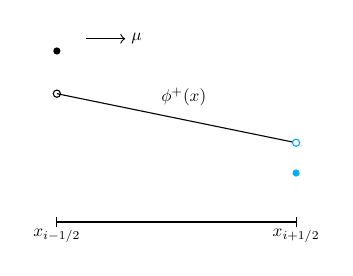
\begin{tikzpicture}[scale=0.62, every node/.style={transform shape}]
            \draw (1.0,4.0) node[fill,circle,inner sep=0pt,minimum
            size=4.2pt] {};
            \draw [->] (1.6,4.25) -- (2.4,4.25) node[anchor=west] {$\mu$};
            \draw (1.0,0.4) -- (1.0,0.6) node[below, pos=0.4] {$x_{i-1/2}$};
            \draw (5.90,0.4) -- (5.90,0.6) node[below, pos=0.4] {$x_{i+1/2}$};
            \node at (3.6,3.06) {$\phi^+(x)$};
            \draw [thick] (1.0,0.5) -- (5.9,0.5) node[anchor=north west] {};
            \filldraw[color=black, fill=white] (1,3.1250) circle (2.1pt);
            \draw (1.0,3.125) -- (5.90,2.120);
            \filldraw[color=cyan, fill=white] (5.9,2.120) circle (2.1pt);
            \draw (5.9,1.5) node[cyan,fill,circle,inner sep=0pt,minimum size=4.2pt] {};
        \end{tikzpicture}
    }}
    \caption{Linear doubly-discontinous representation for mean intensity in LO equations,
    for $\mu>0$.}
    \label{fig:ldd_space}
\end{figure}


\subsection{Issues with ECMC for Spatial Closure}
\label{sec:ecmc_issues}
There are several issues with ECMC that cause the LO moments to not exactly preserve
the HO moments, even for a linear problem.  With ECMC, global and, particularly, local
energy balance are generally not preserved.  For standard MC, there
are source biasing techniques (e.g., systematic
sampling) that exactly preserve the local zeroth moment of the
source and thus satisfy the local balance equations~\cite{shultis_mc,wollaber_review}). 
However, for our HOLO method, even with standard MC we have to reconstruct the bilnear moment
of $x$ and $\mu$, so the consistency terms lead to LO equations that do not exactly
preserve the first moment of the HO solution\footnote{It was verified that with
standard MC, systematic sampling, no analog sampling, and a closure that is only a
function of the zeroth moment, the LO solution exactly reproduces the HO moments, for
a linear problem}.  One final reason is that the analog treatment of absorption for
particles below the weight cutoff (e.g., see Sec.~\ref{sec:tallies}) results in
$\sigma_a \phi^{HO}_i$ and the amount of energy removed from a cell during MC
transport to not be equal; this is due to statistical noise in the path-length
estimators for $\phi^{HO}_i$.  However, ECMC will preserve balance to the order of
the iterative error and statistical noise, so the closure parameters will reproduce
the HO moments to the accuracy of the LO solution.  

\section{Test Problems}

To investigate the utility of the face closures we compare to the LD spatial
closure for two test problems.  We are interested in the accuracy of the solution and
consistency between the HO and LO solutions, particularly for coarser meshes. 
The consistency for the $(l)$-th particular simulation is measured with the relative L$_2$ norm
of the difference between the projected HO and LO solutions, i.e.,
\begin{equation}
    \|\phi_{HO} - \phi_{LO}\|^{(l)}_{2,rel} = \frac{\ds \sqrt{\int_0^X \left(
        \phi_{HO}^{(l)}(x) - \phi_{LO}^{(l)}(x) \right)^2 \dd x}}{\ds \sqrt{
            \int_0^X \left(\phi_{LO}^{(l)}(x)\right)^2 \dd x }}
\end{equation}
where $\phi_{LO}(x)$ and $\phi_{HO}(x)$ are the LDFE representations in space of the
intensity from the HO and LO solvers, from the end of the last time step.
The error between a reference solution and a fine solution for the ${(l)}$-th simulation
is computed as
\begin{equation}
    \|e\|^{{(l)}}_{2,rel} = \frac{\|\phi_{LO}^{n+1,{(l)}}(x) -
    \phi_{LO}^{n+1,ref}\|}{\|\phi_{LO}^{n+1,ref}\|}
\end{equation}
All L$_2$ norms are computed using quadrature over the finest spatial mesh.  An
integrated measure of the error in cell-averaged mean intensities on the mesh of the
$l$-th simulation, with $N_c^{(l)}$ spatial cells, is computed as
\begin{equation}
    \|e\|^{{(l)}}_{a,rel} = \left({\frac{\ds \sum\limits_{i=1}^{N^{(l)}_c}
    \left(\phi_i^{n+1,{(l)}} - \phi_i^{n+1,ref}
\right)^2}{\ds \sum\limits_{i=1}^{N^{(l)}_c}\left(\phi_i^{n+1,ref}\right)^2}}\right)^{1/2},
\end{equation}
where $\phi_i^{n+1,ref}$ is computed by spatially averaging the fine mesh solution over
the $i$-th coarse spatial cell.

The sample mean of each of the above metrics is estimated based on 20 independent
simulations; the sample standard deviation for each \emph{mean} is also reported, e.g.,
\begin{equation}
    s\left(\|e\|_{2,rel}\right) = \left[\frac{1}{20-1}\sum_{l=1}^{20} \left(
    \|e\|_{2,rel}^{(l)} - \|e\|_{2,rel} \right)^2\right]^{1/2},
\end{equation}
where $\|e\|_{2,rel}=\sum_{l=1}^{20}\|e\|_{2,rel}^{(l)}/20$ is the mean.

\subsection{Smooth Problem}

For this problem, the radiation and material energies are initially in
equilibrium at $0.01$ keV.   An isotropic incident intensity of 50 eV is applied
at $x=0$; the incident intensity on the right boundary is $10$ eV.
The material properties are $\rho = 1$ g cm$^{-3}$, $c_v = 0.2$ jks/keV-g, and
$\sigma_a=10$ cm$^{-1}$.
The simulation end time is 0.5 sh.  The time step size increases by 10\% each time step
until the maximum step size of 0.01 sh is reached, beginning from $\Delta t = 0.001$ sh.
This problem is intended to have less steep gradients in the intensity by having constant constant cross
sections, a smaller boundary source, and diffusive problem parameters.
The problem has a smaller optical thickness than other problems tested so that the face-based solutions can be efficiently
estimated, but the small c$_v$ value makes the solution relatively diffusive.  This
problem did not require the lumped relation to produce positive solutions.
However, when projecting from a refined mesh back to the coarse mesh, it was
necessary to rotate the solution to be positive.

All simulations of this problem used 585,900 histories divided over 9 ECMC
batches;  beginning from 30,000 histories and $10$ $\mu$ cells, 30\% of cells were
adaptively refined every third batch, and the number of histories is increased to
keep the average number of histories per cell constant. 
We have have performed two outer HOLO iterations over each time step for all cases; it was
found that additional iterations did not increase consistency, because of the  magnitude
of statistical noise.  Relative convergence of HOLO iterations was below 10$^{-3}$
for two iterations for all cases.  
Fig.~\ref{fig:smooth_compare} compares cell-averaged radiation temperatures for various spatial closures at
coarse mesh sizes and a fine-mesh solution.  The HO spatial closures curve is for the
scaled-slope closure given by Eq.~\eqref{eq:cl_slope}.  There was visually
no difference in the results between the scaled-averaged, scaled-slope, or LD closure. A step closure in all cells
was inaccurate for this problem.

Table~\ref{tab:smooth} compares the different error metrics for different spatial
closures and numbers of cells.  The reference solution for all calculations was the average of 10 simulations with $N_c=500$ spatial
cells.  In all cases, the HO spatial closure produces higher accuracy in the L$_2$
norms and greater consistency between the solvers.  However, there is not an
improvement in accuracy of the cell-averaged intensities.  Neglecting noise, the LDFE representation can be third order
accurate for the $\|e\|_a$ norm and second-order accurate in the L$_2$ norm~\cite{morel_ldtrt}. 
The statistical noise induced in face tallies makes the
additional accuracy that the MC transport can use not greater than the benefit of
higher spatial integration by the MC transport.  It
is noted that, overall, there is very low statistical noise in each of these
solutions due to the ECMC method and relatively high number of histories; at lower
history counts, the small gains of the HO spatial closure will degrade and stability
becomes an issue.

\begin{figure}[H]
    \centering
    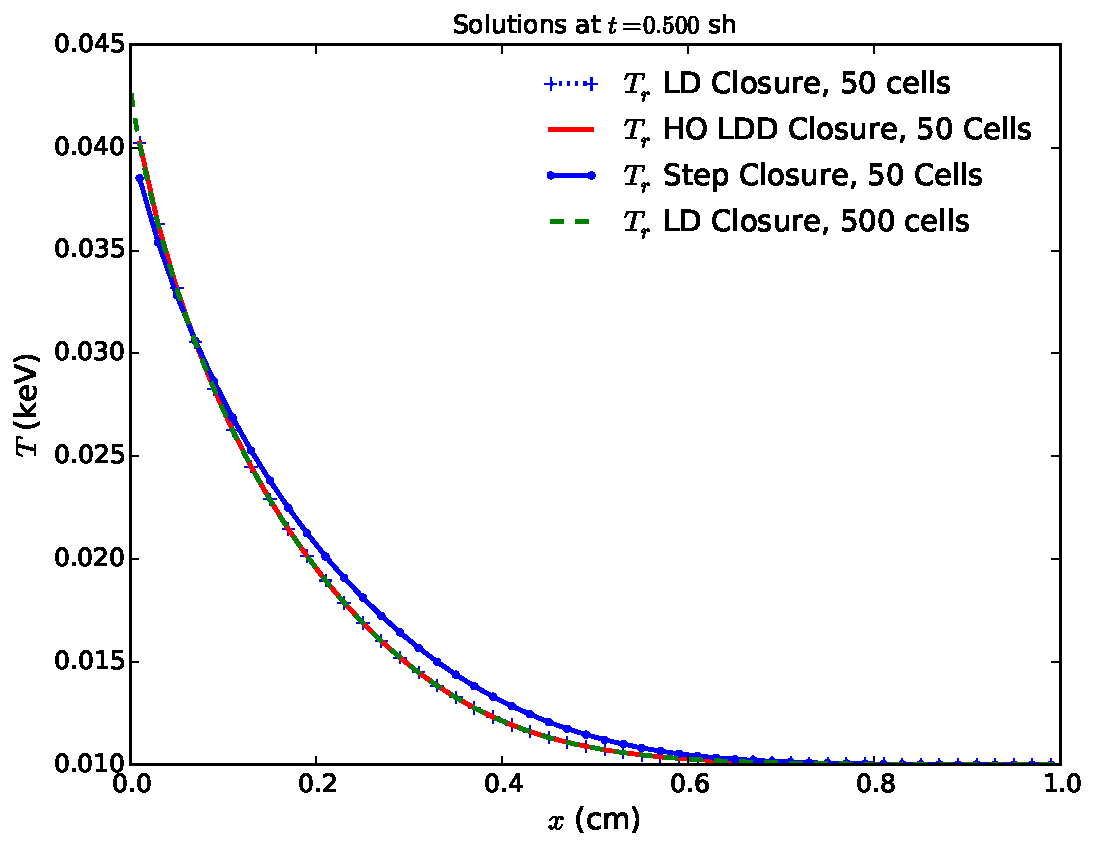
\includegraphics[width=0.99\linewidth]{smooth_compare.pdf}
    \caption{\label{fig:smooth_compare} Comparison of solutions for different spatial closures.}
\end{figure}

\begin{table}[H]
    \caption{\label{tab:smooth} Comparison of error metrics, reported as percentages, averaged over 20 simulations of smooth problem.  The absolute
standard deviation for each value is reported in parenthesis. Reference solution uses 500 cells.}
    \begin{tabular}{|l|cl|cl|cl|} \hline
        Spatial Closure & \multicolumn{2}{|c|}{$\|e\|_2$}  & \multicolumn{2}{|c|}{$\|e\|_{a}$} & \multicolumn{2}{|c|}{$\|\phi^{HO}
        -\phi^{LO}\|_{2}$} \\  \hline \hline
        \multicolumn{7}{|c|}{$N_c = 20$ cells} \\ \hline
LDFE               &   6.60\%  &   (0.17\%)  &   2.80\%     &   (5.7e-03\%)  &   2.90\%   &  (8.1e-03\%)  \\
HO: Scaled Slope   &   6.10\%  &   (2.9e-03\%)  &   3.50\%  &   (5.8e-03\%)  &   0.021\%  &  (8.6e-03\%)  \\
HO: Scaled Average &   6.10\%  &   (2.7e-03\%)  &   3.50\%  &   (5.0e-03\%)  &   0.023\%  &  (1.1e-02\%)  \\ \hline
       \multicolumn{7}{|c|}{$N_c  = 50$ cells}   \\ \hline
LDFE               &   1.60\%  &   (7.9e-04\%)  &   0.59\%  &   (3.8e-03\%)  &   0.76\%)  &  (4.8e-03\%)  \\
HO: Scaled Slope   &   1.40\%  &   (1.5e-03\%)  &   0.67\%  &   (3.2e-03\%)  &   0.012\%  &  (4.0e-03\%)  \\
HO: Scaled Average &   1.40\%  &   (1.5e-3\% ) &   0.67\%   &   (3.1e-03\%)  &   0.013\%  &  (3.9e-03\%)  \\ \hline
       \multicolumn{7}{|c|}{$N_c  = 100$ cells}   \\ \hline
LDFE               &   0.53\%  &   (2.1e-03\%)  &   0.15\%  &   (2.5e-03\%)  &   0.30\%)  &  (9.7e-03\%)  \%\\
HO: Scaled Slope   &   0.45\%  &   (1.5e-03\%)  &   0.16\%  &   (4.6e-03\%)  &   0.012\%  &  (4.8e-03\%)  \\
HO: Scaled Average &   0.45\%  &   (1.4e-03\%)  &   0.16\%  &   (4.7e-03\%)  &   0.012\%  &  (3.6e-03\%)  \\ \hline
    \end{tabular}
\end{table}



\section{Two Material Problem}

The HO spatial closures were applied to solution of the two material problem detailed in Sec.~\ref{sec:two}.
For these results, the time step size is increased from 0.001 sh to a maximum step of 0.01 sh by 5\% each
step, with the final step adjusted to end at 2 sh.

The scaled-slope closure was found to not stably converge, even for 3 batches of 10$^6$
histories.  This coudl be caused the steep gradients at the foot of the wave.  As the
solution slightly overshoots, the slope changes signs between cells. 




\chapter{\uppercase {The High-Order Exponentially-Convergent Monte Carlo Solver}}

\section{The ECMC High Order Solver}

The transport equation to be solved by the HO solver is
\begin{equation}\label{eq:ho_base}
\mu \pderiv{I^{n+1,k+1/2}}{x} + \left(\sigma_t^k + \frac{1}{c \Delta t }\right)
I^{n+1,k+1/2}
= \frac{\sigma_s}{2} \phi^{n+1,k} +\frac{1}{2} \left(\sigma_a^k a c T^4
\right)^{n+1,k} + \frac{\tilde I^n}{c\Delta t} 
\end{equation}
where the superscript $k$ represents the outer HOLO iteration index.  Material property indices will be
suppressed from now on.  Here, $k+1/2$ denotes the
ECMC solution within outer HOLO iteration $k$, whereas $k$ and $k+1$ represent successive LO
solves. The sources at $k$ in Eq.~\eqref{eq:ho_base} are estimated by the previous LO solution. Cross sections are
evaluated at $T^{n+1,k}$.  As all sources on the right side of the equation are known,
this defines a fixed-source, pure absorber transport problem.  We will solve
this equation using ECMC.  A more detailed description of the
ECMC method can be found in~\cite{jake}, but a brief overview is given here.  A general proof of exponential convergence for related adaptive MC transport methods with a different formulation is depicted in~\cite{spanier_mc}.

 In operator notation, Eq.~\eqref{eq:ho_base} can be written as
\begin{equation}\label{te_oper}
\B L^k I^{n+1,k+1/2}  = q^{k}
\end{equation}
where $I^{n+1,k+1/2}$ is the transport solution of the angular intensity based on the
$k$-th LO estimate of $q^k$.
The linear operator $\B L^k$ is the continuous streaming plus
removal operator defined by the left hand
side of Eq.~\eqref{ho_trans}.
The $m$-th approximate LDFE solution to Eq.~\eqref{te_oper} ($m$ is the index of inner HO
batches) is represented as
$\tilde{I}^{n+1,(m)}$.    
The $m$-th residual is defined as $r^{(m)} = q - \B L^k\tilde{I}^{n+1,(m)}.$ 
For reference, the residual at iteration $m$ in the HO solve
is
\begin{equation}\label{eq:resid}
r^{(m),k+1/2} = \frac{\sigma_s}{2} \phi^{n+1,k} +\frac{1}{2} \left(\sigma_a a c T^4
\right)^{n+1,k} + \frac{\tilde{I}^n}{c \Delta t } -
\left(\mu \pderiv{\tilde{I}^{n+1,k+1/2}}{x} +
\left(\sigma_t + \frac{1}{c \Delta t }\right) \tilde{I}^{n+1,k+1/2}\right)^{(m)}
\end{equation}
where the $k$ terms are LD in space on the coarsest mesh and are not recalculated at any point during
the HO solve. The functional form of $\tilde{I}^n$ is defined from the final HO
solution of the previous time step.  

Addition of $\B L I^{n+1} - q=0$ to the residual equation 
and manipulation of the result yields the error equation
\begin{equation}\label{eq:err_eq}
    \B L (I^{n+1} - \tilde{I}^{n+1,(m)}) = \B L {\epsilon}^{(m)} = r^{(m)}
\end{equation}
where $I^{n+1}$ is the exact solution and ${\epsilon}^{(m)}$ is the true error in
$\tilde{I}^{n+1,(m)}$. 
We have suppressed the HOLO iteration indices because the LO estimated $q^{k}$ and $\B L^{k}$ remain constant over the entire HO solve.
The $\B L$ operator in the above equation is inverted yielding
the Monte Carlo LDFE projection of the error in $\tilde{I}^{n+1,(m)}$, i.e., 
\begin{equation}\label{eq:mc_err}
\tilde{\epsilon}^{(m)} = \B L^{-1} r^{(m)}
\end{equation}
where $\B L^{-1}$ is the Monte Carlo inversion of the streaming and removal operator.  
This inversion is strictly a standard Monte Carlo simulation.   It is noted that the exact
error in $\tilde{I}^{n+1,(m)}$ (with respect to Eq.~\eqref{eq:ho_base}) is being estimated with MC;
%in Because $\B L$ in Eq.~\eqref{eq:err_eq} is the continous operator and $\B
%L^{-1}$ represents the analytic inverse of $\B L$~\cite{shultis_mc}, the exact error
tallies produce a projection of the error onto a LDFE space-angle trial space. The space-angle
moments of the error computed as $\tilde{\epsilon}^{(m)}$ can be added to the
moments of $\tilde{I}^{n+1}(m)$ to produce a more accurate solution.  


Here, we emphasize the solution $\tilde{I}^{n+1,(m)}$ represents the LDFE projection of the exact Monte Carlo
solution to the transport problem defined by Eq.~\eqref{eq:ho_base}.  The discretization error is in $q$, i.e., the LD spatial
representation of the emission and scattering source and the LDFE space-angle projection $\tilde I^{n}(x,\mu)$.
 The projection of the intensity is in
general far more accurate than a standard finite element solution, e.g., a S$_N$ collocation method in angle.  In typical IMC calculations, the average
energy deposition within a cell is computed using a standard path-length volumetric
flux tally; the zeroth moment of the LDFE projection of ${\epsilon}$ is
computed using an equivalent tally, preserving the zeroth moment of the true error.

Volumetric flux tallies over each space-angle element are required to estimate
$\tilde{\epsilon}^{(m)}$.  The LD approximation in space is used to relate the
outflow within a cell to the volumetric moments, eliminating the need for
face-averaged tallies.  The procedure for representing the solution, sampling with negative and
positive weight particles, and tally
definitions are given in Appendix~\ref{app:tallies}.

The ECMC algorithm is
\begin{enumerate}
    \item Initialize the guess for $\tilde{I}^{n+1,(0)}$ to $\tilde{I}^{n}$ or the
        projection of $\tilde{I}^{n+1}$ from the latest HO solve
\item Compute $r^{(m)}$.
\item Perform a MC simulation to obtain $\tilde{\epsilon}^{(m)} = \B L^{-1} r^{(m)}$
\item Compute a new estimate of the intensity $\tilde I^{n+1,(m+1)} = \tilde I^{n+1,(m)}
+ \tilde\epsilon^{(m)}$
\item Repeat steps 2 -- 4 until desired convergence criteria is achieved. 
\end{enumerate}
The initial guess for the angular intensity $I^{n+1,(0)}$ is computed based on the previous solution
for $\tilde{I}^{n}$. This is a critical step in the algorithm; it significantly reduces the required number of
particles per time step because the intensity does not change drastically between time steps in
optically-thick regions.  It is noted that the ECMC batch (steps 1-4 of the
algorithm) results in essentially the same estimate of the solution as the residual
formulation used in~\cite{rmc}.  The primary difference is that our method uses an LDFE trial
space and iterates on the solution estimate by recomputing the residual.

Exponential convergence is obtained if the error $\epsilon$ is reduced each batch.  With each batch, a
better estimate of the solution is being used to compute the new residual, decreasing
the magnitude of the MC residual source at each iteration $m$, relative to the solution
$I^{n+1}$.  Each MC
estimate of the moments of $\epsilon$ still has a statistical uncertainty that is
governed by the standard $1/\sqrt{N}$ convergence rate~\cite{shultis_mc}, for a
particular source $r^{(m)}$, where $N$ is the number of histories performed.  If the statistical estimate of the projection $\tilde\epsilon$ is not sufficiently
accurate, then the iterations would diverge. It is noted that there is statistical correlation across batches because
$I^{n+1,(m+1)}$ and $\epsilon^{(m)}$ are correlated through $I^{n+1,(m)}$ and the MC source $r^{(m)}$.  
%Although th
%variance in tallies of $\epsilon^{(m)}$ can be estimated with the sample variance of
%histories, the variance in the moments of $I^{n+1,(m+1)}$ cannot be easily
%estimated due to the correlation between $I^{n+1,(m)}$ and the source
%$r^{(m)}$.

Because the exact angular intensity does not in general lie within the LDFE trial space, the
iterative estimate of the error will eventually stagnate once the error cannot be sufficiently
represented by a given FE mesh.  An adaptive $h-$refinement algorithm has been
implemented that can be used to allow the system to continue converging towards the
exact solution~\cite{jake,ans_2014}. For TRT problems where absorption-reemission physics dominate, the diffusive and slowly varying
regions of the problem require a less refined angular mesh to capture the solution than typical neutronics
problems.  However, greater spatial resolution is needed due to steep spatial
gradients.   
Once error stagnation has occurred (and mesh refinement has reached a maximum level),
additional histories can be performed with a
fixed residual source to estimate the remaining error in the current solution.  Although the remaining error will
converge statistically at a standard $1/\sqrt{N}$ convergence rate, the remaining
error will be much smaller than for a standard MC simulation, producing a much more
efficient solution method overall.

For the HO solver, in cells near the radiation wavefront, the LDFE trial space results in
negative values in $\tilde{I}^{n+1}(x,\mu)$, similar to the LO solver.  Because the residual formulation in ECMC allows for negative weight
particles to occur, currently we do not treat these cells specially.  We detect if
the consistency terms lie in the appropriate half space at the end of the HO solve,
an indication that the intensity was negative within that cell.  If the terms are non-physical, then
they are replaced with the corresponding S$_2$-equivalent value. In general,
in such cells where the trial space cannot accurately represent the solution, error stagnation will
rapidly occur. 

\section{MC solution with LDD trial space}
\label{sec:ldd_mc}

The inclusion of the outflow discontinuity has a minimal effect on the treatment of the
residual source. The residual source and process of estimating moments of
the error on the interior of a space-angle cell is unchanged.  The process of estimating
the solution on the outgoing face requires tallying the solution when particles leave a
cell. The tallying process is discussed later in Section~\ref{sec:face_tallies}.  

Applying $L$ to the LDD trial space, as shown in Fig.~\ref{fig:ldd}, results in two $\delta$ functions at each interior face.
For positive flow, at a face $x_{i+1/2}$, the face portion of the residual is defined as
\begin{align}
    \label{eq:res_face}
    \rface(x_{i+1/2}) &= -\mu \pderiv{\tilde I^{(m)}}{x}\big|_{x_{i+1/2}}\\
    &= \rface(x_{i+1/2}^-)\delta^-(x - x_{i+1/2}) + \rface(x_{i+1/2}^+)\delta^+(x - x_{i+1/2}) 
\end{align}
where
\begin{align}
    \rface(x_{i+1/2}^-) &= -\mu\left( \tilde I^{(m)}(x_{i+1/2},\mu) - \tilde I^{(m)}(x_{i+1/2}^-,\mu)
           \right)\\
    \rface(x_{i+1/2}^+) &= -\mu\left( \tilde I^{(m)}(x_{i+1/2}^+,\mu) -
           \tilde I^{(m)}(x_{i+1/2},\mu)
           \right).
\end{align}
Here, $I^{(m)}(x_{i+1/2}^+)$ and $I^{(m)}(x_{i+1/2}^-)$ are the LD solution extrapolated to $x_{i+1/2}$ from the
$x$ cell $i$ and cell $i+1$, respectively.
Particles sampled from the two $\delta$-functions have the same starting location.  The
only difference is, for positive $\mu$,  particles sampled from $\rface(x^-_{i+1/2})$ will
contribute to the face tally at $x_{i+1/2}$; the opposite is true for negative $\mu$.

To reduce variance, we do not sample the two $\delta$ functions independently.
%or score contributions to the outflow face from the interior face source. 
Instead, we combine the
two $\delta$-functions into a single face source,
do not score particles at the face from which they are sampled.  To account for the
untallied error, we add the analytic
contribution to the error from the face source to the corresponding face at the end of a batch.
It is noted the combination of the two $\delta$-functions produces the same residual source as the
original LD residual.

Define the additional error contribution 
from the face sources at $x_{i+1/2}$ as $\dep$.  This additional error is tallied
everywhere by MC, except for at $x_{i+1/2}$.  The transport equation satisfied by $\dep$, for positive
$\mu$, with effective total cross 
section $\hat \sigma_t$, is
\begin{equation}
    \label{eq:ho_face}
    \mu \pderiv{\dep}{x} + \hat\sigma_t \dep = \rface(x_{i+1/2}^-)\delta^-(x - x_{i+1/2}) + \rface(x_{i+1/2}^+)\delta^+(x - x_{i+1/2}) 
\end{equation}
This equation is integrated from $x_{i+1/2}-\alpha$ to $x_{i+1/2}$ to produce
\begin{multline}
    \mu\dep(x_{i+1/2},\mu) - \mu\dep(x_{i+1/2}-\alpha,\mu)  + \int\limits_{x_{i+1/2}-\alpha}^0 
    \hat \sigma_t \dep \dd x  \\ =  \rface(x_{i+1/2}^-) +
        \int\limits_{x_{i+1/2}-\alpha}^0\rface(x_{i+1/2}^+)\delta^+(x - x_{i+1/2}) \dd x.
\end{multline}
The integral on the right side of the equation is zero because $\delta^+(x-x_{i+1/2})$ is
zero for $(-\infty,x_{i+1/2}]$.  The limit of the above equation is taken as $\alpha\to0$, i.e.,
\begin{multline}
    \lim_{\alpha\to0}\left( \mu\dep(x_{i+1/2},\mu) - \mu\dep(x_{i+1/2}-\alpha,\mu)  + \int\limits_{x_{i+1/2}-\alpha}^0 
    \hat \sigma_t \dep \dd x \right)  = \lim_{\alpha\to0} \rface(x_{i+1/2}^-) 
\end{multline}
The integral goes to zero because $\dep$ is smooth on the interior of the cell, and
$\mu\dep(x_{i+1/2}-\alpha,\mu)$ goes to zero because there is no source upstream of
$x_{i+1/2}^-$. Thus, the final solution is
\begin{equation}
    \dep(x_{i+1/2},\mu) = \frac{\rface(x_{i+1/2}^-)}{\mu} = 
     \tilde I^{(m)}(x_{i+1/2}^-,\mu) - \tilde I^{(m)}(x_{i+1/2},\mu)
.
\end{equation}
The update for $I(x_{i+1/2},\mu)$ is 
\begin{align}
   \tilde I^{(m+1)}(x_{i+1/2},\mu) &= \tilde I^{(m)}(x_{i+1/2},\mu) + \epsilon^{(m)}(x_{i+1/2},\mu) +
    \dep(x_{i+1/2},\mu) \\ 
        &= \tilde I^{(m)}(x_{i+1/2}^-,\mu) + \epsilon^{(m)}(x_{i+1/2},\mu).
\end{align}
This result has the peculiar effect that the estimation of the solution on a face depends only on
the interior solution $\tilde I^{(m)}(x_{i+1/2}^-,\mu)$ and not the previous face value 
$\tilde I^{(m)}(x_{i+1/2},\mu)$. This could be used to only estimate
face values in particular cells, at any chosen batch.



\section{Implementation of ECMC finite-element space, tallies, and residual sampling}
\label{app:tallies}

The ECMC solver uses a finite element representation in space and angle. On the
interior of the cell with the $i$-th spatial index and $j$-th angular index, the linear representation is defined as
\begin{equation*}
    \tilde I(x,\mu) = I_{a,ij} + \frac{2}{h_x}I_{x,ij}\left(x-x_i\right) +
    \frac{2}{h_\mu}I_{\mu,ij}\left(\mu-\mu_j\right), \quad x_\il <  x < x_\ir,\quad
     \mu_\jl \leq \mu \leq \mu_\jr
\end{equation*}
The spatial cell width is $h_x$, the angular width is
$h_\mu$, the center of the cell is $(x_i,\mu_j)$, and
\begin{align}\label{app1}
    I_{a,ij} &= \frac{1}{h_x h_\mu} \iint\limits_{\mathcal{D}} I(x,\mu)\, \dd x \dd \mu \\
    I_{x,ij} &= \frac{6}{h_xh_\mu}\iint\limits_{\mathcal{D}} \left(\frac{x - x_i}{h_{x}}\right)
    I(x,\mu)\, \dd x \dd \mu \\ \label{app2}
    I_{\mu,ij} &= \frac{6}{h_xh_\mu}\iint\limits_{\mathcal{D}}
     \left(\frac{\mu - \mu_j}{h_{\mu}}\right)
    I(x,\mu)\, \dd x \dd \mu,
\end{align}
where $\mathcal{D}: x_\il \leq  x \leq  x_\ir \times \mu_\jl \leq \mu \leq \mu_\jr$.
%$I_a$ is the cell average intensity, and $I_\mu$ and $I_x$ define the
%the first moment in $\mu$ and $x$ of the intensity, respectively. 
Standard upwinding in space is used to
define $I(\mu)$ on incoming faces. 

This representation can directly be plugged into
Eq.~\eqref{eq:resid} and evaluated to produce the residual source in the ECMC HO transport
problem.  The MC source $r^{(m)}(x,\mu)$ in Eq.~\eqref{eq:mc_err}
consists of both face and volumetric sources and can produce positive and
negative weight particles.  The distribution for sampling particle coordinates, in space and angle, is based on the $L_1$
norm over space and angle of the residual~\cite{jake}.  A particular cell volume or face 
is sampled, and then rejection sampling~\cite{shultis_mc} is used to sample from
the appropriate distribution on the face or interior of the space-angle cell.  If the
residual is negative at the sampled coordinates, the weight of the particle history is negative.

During a MC batch, moments of the error are tallied.  The necessary moments of the error are
defined analogously to Eq.'s~\eqref{app1}--\eqref{app2}.
The tallies are evaluated by weighting the particle density with the appropriate
basis function and integrating along the history path through the cell.  For the cell average, the $n$-th
particle makes the contribution
\begin{equation}
   \epsilon^n_{a,ij} = \frac{1}{h_xh_\mu} \int\limits_{s^n_o}^{s^n_f}  w^n(x,\mu) \dd s,
\end{equation}
where $s_o^n$ and $s_f^n$ are the beginning and end of the $n$-th particle track in the cell and $w(x,\mu)$ is
the weight of the error particle in the MC simulation.  Weight is attenuated exponentially, i.e., $w(x,\mu)\propto
\exp(-\sigma_t|x/\mu|)$.
Substitution of the exponential attenuation of the weight produces the result
\begin{equation}
    \epsilon^n_{a,ij} = \frac{w(x_0,\mu)}{\sigma_t h_x h_\mu} \left(1 -
    e^{-\sigma_ts^n}\right).
\end{equation}
Here, $w(x_0,\mu)$ is the particle weight at the start of the path and $s^n$ is the
length of the track. The contribution of a
particle track to $\epsilon_x$ is given by
\begin{equation}
    \epsilon^n_{x,ij} = \frac{w(x_0,\mu)}{h_x^2h_\mu \sigma_t} \left[x_0 - x_f e^{-\sigma_t s^n}
        + \left(\frac{\mu}{\sigma_t} - x_i \right)\left(1-e^{-\sigma_t s^n}\right),
    \right]
\end{equation}
where $x_0$ and $x_f$ are the beginning and ending $x$ coordinates of the $n$-th
path.  The contribution to the first moment in $\mu$ is 
\begin{equation}
    \epsilon^n_{\mu,ij} = \frac{w(x_0,\mu)}{h_{\mu}^2h_x\sigma_t}\left(\mu -
    \mu_j\right) \left(1 - e^{-\sigma_ts^n}\right),
\end{equation}
where the particle $x$-direction cosine $\mu$ does not change because it is a pure-absorber simulation.
Finally, the moments of the error are simply the average contribution of all particles.

\section{Adaptive Mesh Refinement}
\label{app:refinement}
This section describes the adaptive refinement strategy for the ECMC algorithm.
Detailed equations for performing projections between meshes and computing the residual source on
the refined meshes can be found in~\cite{jake}.  At the end of the ECMC batch,
refinement is performed in space-angle cells based on a jump indicator.  The jump
indicator is the magnitude of the different between $I(x,\mu)$ in adjacent cells,
averaged over each edge.  The value of the largest jump, out of the four edges within a
cell, is used as the
indicator for that cell.  Based on this indicator, the 20\% of cells with the largest jump are
refined.  Future work will explore simply using $\epsilon$ to indicate refinement,
rather than the jump error.  The refinement of a cell is chosen to be symmetric, with each space-angle cell divided into four
equal-sized cells.  The solution for $\tilde{I}^{n+1}(x,\mu)$ of the batch is projected onto
the finer mesh for the next batch. Because the dimensionality of the sample space has
increased, we increase the number of histories per batch s.t. the ratio of the number
of histories to total cells is approximately constant for all meshes.  At the end of the last HO solve in a time step,
$\tilde{I}^{n+1}$ is projected back onto the original, coarsest mesh and stored as
$\tilde{I}^{n}$ for the next time step.



\subsection{Variance Reduction and Source Sampling}


As in~\cite{park}, because we are solving a pure absorber problem with Monte Carlo, we will allow
particles to stream without absorption to reduce statistical 
variance in the tallies.  The weight of particles is reduced deterministically along
the path as they stream, with no need to sample a path length.  Because particles are exponentially attenuated, the normalized weight is
adjusted as $w(x,\mu) = w(x_0,\mu)\exp(-\sigma_t|(x-x_0)/\mu|)$, where $x_0$ is the starting location of the path.  The tallies account
for the continuously changing weight, as given in Appendix~\ref{app:tallies}. Histories are allowed to stream in this manner for 6 mean free paths (mfp))
before switching to analog path length sampling; this limits the tracking of very small weight histories. The choice of 6 mfp allows particles to 
continuously deposit weight until they reach 0.25\% of their original weight.  Path lengths are tracked in terms of mfp, so there is no need to resample at material
interfaces.

As another way to improve efficiency, a modified systematic sampling
method~\cite{shultis_mc} was used for determining source particle locations.  The goal is
to effectively distribute particle histories to regions of importance, but to sample a
sufficient number of histories in less probable regions to prevent large statistical
noise.  However, there is no need to sample histories in regions in thermal equilibrium.
The residual gives a good indication of where histories are most likely to contribute to
the error, particularly in optically thick cells where particles do not transport long
distances.   In
the sampling algorithm the number of particle histories sampled in each space-angle cell
is predetermined and proportional to the magnitude of the residual, including face and
volumetric sources, within that cell.  Then, for the predetermined number of histories
within a cell, the source location is randomly sampled according to the residual source
distribution of that cell.  In cells where the relative magnitude of the residual is on the order of roundoff no particle histories are sampled. In these 
regions the problem is remaining in equilibrium and the solution is known exactly.  For
cells that are significant, but have a predetermined number of histories below some preset
minimum $N_{min}$, the number of histories sampled in that cell is set to $N_{min}$. This
is to limit bad statistics in low probability cells (this would be important for
adaptively refined meshes).  In the simulations performed for this work $N_{min}=1$.  This
choice was made to keep the total number of histories per time step constant throughout
the simulation for comparison to IMC. 

%The unmodified probability of a particle being born in cell $j$ is 
%\begin{equation}
%p_j = \frac{||r^{(m)}_j||}{||r^{(m)}||}
%\end{equation}
%Thus, the number of
%particles in cell $j$ is 
%\begin{equation}
%N_j = 
%\left\{\begin{matrix}
% \lfloor(Np_j)\rfloor, & Np_j > N_{\min}
%\\ 0, & \frac{p_j}{1/N_c} < p_{cut}
%\\ N_{min}, & \text{else}
%\end{matrix}\right.
%\end{equation}
%where $N_{\min}$ is the minimum number of histories in significant cells, $N_c$  is the number of cells, and $p_{cut}$ is the chosen relative probability cutoff.
 %This is done by first filling the cells with $N_{min}$ histories and distributing the remaining number of histories proportional to $p_j$.


\chapter{\uppercase{Computational Results}}

We will compare results of the HOLO method to IMC with
a source tilting algorithm for two test problems~\cite{jayenne}.  Also, we
briefly compare performance in Section~\ref{timing}.  For all IMC results, no
local, discrete diffusion acceleration methods for effective scattering
(e.g., those in~\cite{imd,ddmc}) are applied.  Finally,  we will demonstrate
the efficiency advantage of ECMC in our HOLO algorithm by comparing the results
to the same HOLO algorithm if the ECMC algorithm is replaced with a standard
Monte Carlo (SMC) simulation.  Results are also given for the case of a single
ECMC batch, which is similar to a RMC method.

REWRITE:
The lumping-equivalent discretization
discussed in Sec.~\ref{sec:ldfe_fixups} is used for cells where the solution for
$\phi^{n+1}$ becomes negative. When negative values for $\phi^{n+1,\pm}(x)$ are detected, the lumping-equivalent discretization is used within
those cells and that Newton step is repeated.
The cells
nearest the wavefront required use of the lumping-equivalent discretization and
$S_2$ equivalent terms during the LO
solve, resulting in strictly positive solutions.


A measure of variance in cell-averaged scalar intensities was
calculated to provide a quantitative measure of the statistical accuracy of different solution
methods.  To form sample standard deviations, twenty independent simulations for each
particular result were performed using unique random number generator seeds.
The variance of a particular cell-averaged $\phi(x)$ is 
\begin{equation} 
    S_i^2 =  \frac{20}{20-1} \sum_{l=1}^{20} \left(\overline{\phi_{i}} -
    \phi_{i}^l\right)^2,
\end{equation}
where $\phi_{i}^l$ is the cell-averaged scalar intensity for cell $i$ from the $l$-th of 20 independent simulations and
$\overline{\phi_{i}}$ is the corresponding sample mean from the 20 simulations. To
provide a normalized, spatially-integrated result, we form a norm over cells as 
\begin{equation}
    \ss = \left({\frac{\sum\limits_{i=1}^{N_c}
S_i^2}{\sum\limits_{i=1}^{N_c}\overline{\phi_{i}}^2}}\right)^{1/2},
\end{equation}
where $N_c$ is the number of spatial cells. 

We will also form a figure of merit (FOM) to demonstrate how statistical accuracy
scales with the number of histories performed.  Our FOM is defined as
\begin{equation}\label{eq:fom}
    \FOM = \frac{1}{N_{\text{tot}}\ss^2}
\end{equation}
where $N_{\text{tot}}$ is the total number of histories performed over the simulation.
A larger value of the FOM indicates that the method produced less variance in the
solution per history performed, for a given problem.  This form of the FOM
is typically chosen because the variance is expected to reduce inversely proportional
to $N_{\text{tot}}$, so for standard MC simulations the FOM becomes, on average, independent of
$N_{tot}$~\cite{shultis_mc}.  The FOM is not necessarily expected to be independent
of $N_{\text{tot}}$ for IMC or
our HOLO method due to correlation of the solution between time steps; additionally, ECMC
has correlations between batches.

\subsection{Marshak Wave}
\label{sec:marsh}

For the first problem, the radiation and material energies are initially in
equilibrium at $2.5\times 10^{-5}$ keV.   An isotropic incident intensity of 0.150 keV is applied
at $x=0$; the incident intensity on the right boundary is $2.5\times10^{-5}$ keV.
The material properties are $\rho = 1$ g cm$^{-3}$ and $c_v = 0.013784$ jks/keV-g. The
absorption cross section varies as $\sigma(T) = 0.001\;\rho\; T^{-3}$ (cm$^{-1}$), for $T$
in keV.
The simulation was advanced until $t=5$~sh~(1~sh~$\equiv$~10$^{-8}$~s) with a fixed time step size of 0.001 sh. For comparison purposes, we
have not used adaptive mesh
refinement, only performed one HOLO iteration per time
step, and use a fixed 3 HO batches with equal number of histories per batch. A
relative tolerance of $10^{-6}$ for the change in $\phi(x)$ and $T(x)$ was used for
the LO newton solver for all results. Radiation energy
distributions are plotted as an effective temperature given by
$T_r=(\phi/(ac))^{0.25}$.  The effective temperature represents the temperature of the
material, if the material and temperature were in equilibrium.  Cell-averaged quantities are plotted.
Although isotropic scattering is handled by the LO solver in the algorithm described above, we have only
considered problems with $\sigma_s = 0$ here.  Results for neutronics with isotropic
scattering included are given in~\cite{ans_2014}.

\begin{figure}[htb]
    \centering
\begin{subfigure}{0.7\textwidth}
  \centering
    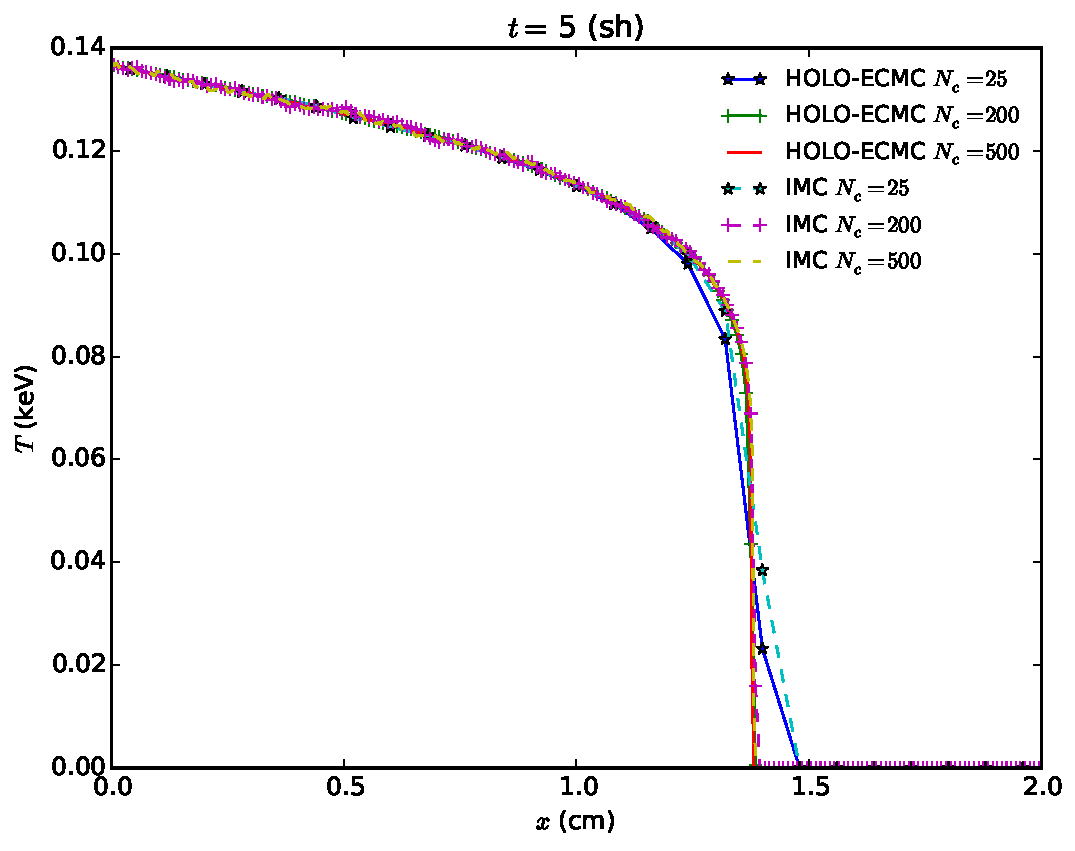
\includegraphics[width=0.99\linewidth]{marshak_mesh_conv.pdf}
    \caption{\label{marshak_mesh_conv} Convergence of IMC and HOLO-ECMC solutions.}
\end{subfigure}
\begin{subfigure}{0.7\textwidth}
  \centering
  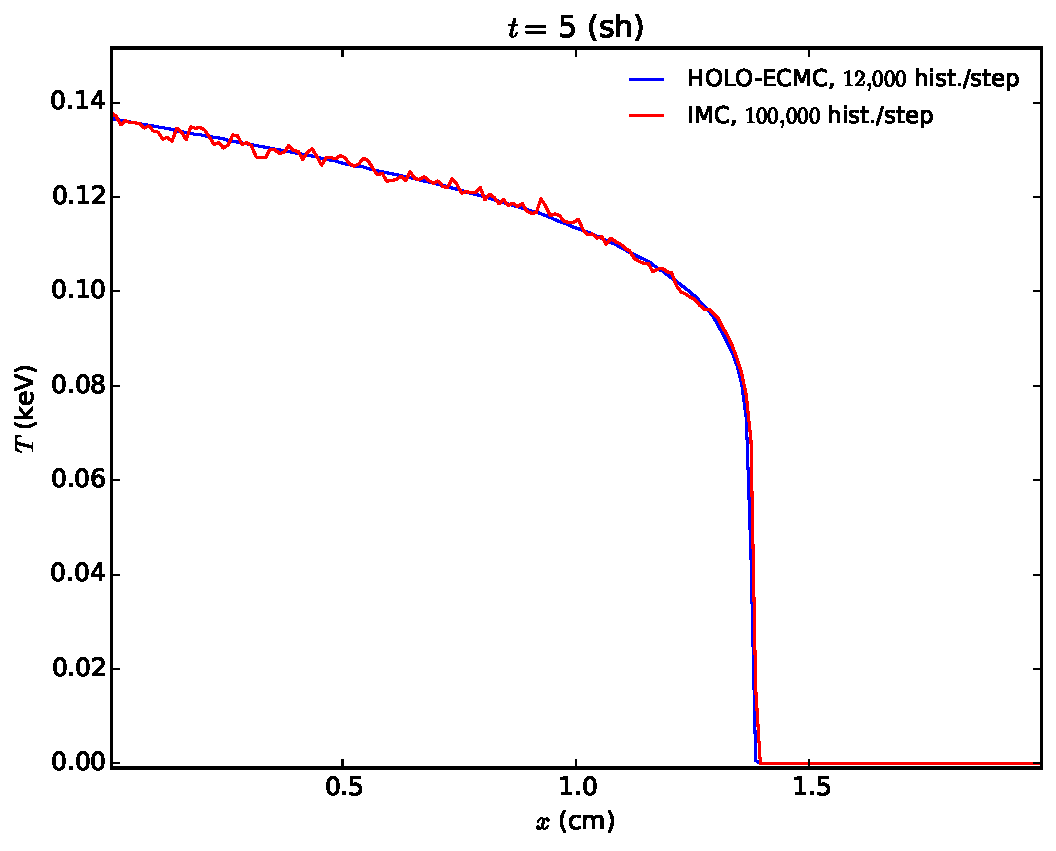
\includegraphics[width=0.99\linewidth]{marshak_200_compare.pdf}
  \caption{\label{marshak_200_compare}  Comparison of solutions for 200 spatial cells. }
\end{subfigure}
\caption{Comparison of radiation temperatures for Marshak wave problem at ${t=5}$ sh.}
\end{figure}

Fig.~\ref{marshak_mesh_conv} compares the cell-averaged radiation temperatures  for the
IMC and HOLO method with ECMC, for various number of spatial mesh cells $N_c$; we
have used HOLO-ECMC to denote our algorithm because later results will use different HO solvers.   For
all IMC calculations, $n=10^5$ histories per time step were used.  For the HOLO method, we have used
4 equal-sized cells in $\mu$ for the finite-element angular mesh used by the ECMC
solver.  The spatial grid is the same for the HO and LO solvers. For the cases
of $N_c=25$ and $N_c=200$, $4,000$ histories per batch ($n=12,000$ per time step)
were used.  For $N_c=500$, 16,000 histories per time step were used due to increased
number of space-angle cells that
need to be sampled. The IMC and HOLO solutions agree as the mesh is converged.  There is
similar agreement in the location of the wavefront due to the linear shape of the emission source over a cell.  The cells
nearest the wavefront required use of the lumping-equivalent discretization and
$S_2$ equivalent terms during the LO
solve, resulting in strictly positive solutions.
 
Fig.~\ref{marshak_200_compare} compares solutions
for the case of 200 cells.  For the IMC solution $10^5$ histories per time step were
simulated; for the HOLO method only $4,000$ histories per batch
(12,000 per time step) were simulated. There is significant statistical noise in the IMC solution
compared to the HOLO solution.  The HOLO solution visually demonstrates no
statistical noise.  Because the ECMC solve is only determining the change over the
time step, the statistical noise in the result is small relative to the magnitude of
$I^{n+1}$.  Also, the source sampling only places particles in cells where the residual is
large.  No particles are sampled in the equilibrium region out front of the wave. 

Table~\ref{marshak_var} compares $\ss$ and the FOM for IMC and the HOLO method, for different
numbers of histories per time step. The FOM results are normalized to the value for IMC with
$n=12,000$.  The HOLO method demonstrates less variance
for the same numbers of histories, producing FOM values that are two orders of magnitude greater than for IMC.  Where as the FOM remains relatively constant for
IMC, as $n$ is increased the FOM improves for the HOLO method.  This is a result of
each batch producing more statistically accurate estimates of the error $\epsilon$,
which results in an increased convergence rate of $\epsilon$ overall.  
\begin{table}[H]
\centering
\caption{\label{marshak_var} \textbf{Comparison of sample statistics for the Marshak Wave problem.   Simulation end time is $\mathbf{t=5}$ sh.}}
\vspace{-0.1in}
\begin{tabular}{|c|cc|cc|}\cline{2-5}
    \multicolumn{1}{c|}{}       & \multicolumn{2}{|c|}{\ss} &
    \multicolumn{2}{|c|}{\FOM} \\ \hline
hists./step   & IMC & HOLO-ECMC &  IMC & HOLO-ECMC   \\ \hline
   12,000	 & 3.40\%  & 0.28\% &  1    &  145      \\
  100,000    & 1.22\%  & 0.057\% & 0.93    &   422     \\ \hline
\end{tabular}
\end{table}



\subsection{Two Material Problem}
\label{sec:two}

This problem consists of an optically thin (left) and an optically thick (right) material region,
with temperature-independent cross sections.  The material properties are given in
Table~\ref{two_mat_props}.  Initially the radiation and material energies are in
equilibrium at a temperature of 0.05 keV.  An isotropic incident intensity of 0.500 keV
is applied at $x=0$ at $t=0$; the isotropic incident intensity on the right boundary is 0.05
keV.  The simulation end time is 5 sh. For all HOLO simulations, we have used 8
equal-sized mesh cells in $\mu$. As for the Marshak problem, the cells nearest the wavefront required use of the lumping-equivalent discretization and
$S_2$ equivalent terms during the LO solve.
\begin{table}[H]
        \caption{Material properties for two material problem\label{two_mat_props}}
\centering
        \begin{tabular}{|c|cc|}  \cline{2-3}
            \multicolumn{1}{c|}{}   & $x \in [0,0.5)$ cm & $x \in [0.5,1.0]$ cm   \\ \hline
            $\sigma_a$ (cm$^-1$)  & 0.2 & 2000 \\
            $\rho$ (g cm$^-3$) & 0.01 & 10.0 \\
            $c_v$ (jks/keV-g) & $0.1$ & $0.1$ \\ \hline
        \end{tabular}
\end{table}
Fig.~\ref{twomat_full} compares the HOLO and IMC radiation 
temperatures at the end of the simulation. The
IMC and HOLO results show good agreement
over the finer mesh.
On the coarse mesh ($N_c=20$), the LDFE representation of $T^4$ in the HOLO method predicts the location of the
wavefront more accurately than the IMC method with source tilting.

Fig.~\ref{compare_ho} demonstrates the benefit of ECMC as a HO solver compared to
standard MC.  The HOLO algorithm
with the ECMC HO solver (HOLO-ECMC) results
are for running 3 batches of 10,000 histories, per time step. The solution for the HOLO method with a standard MC solver as the HO solver
(HOLO-SMC) with standard source sampling uses 10$^5$ histories per time step. The HOLO-SMC solution demonstrates significant
statistical noise.  This noise is introduced into the LO solver by bad statistics in
computing the consistency terms. Also
plotted is an S$_2$ solution obtained with consistency terms that are equivalent
to S$_2$ and no HO correction.  The S$_2$ solution results in an artificially fast
wavefront, as expected, demonstrating the necessity of HO correction in this problem.

Table~\ref{twomat_var} compares the FOM and $\ss$ for IMC and the HOLO-ECMC method.  The FOM
values are normalized to the value for IMC with $n=30,000$.  The end time was reduced
to $2$ sh for these results to reduce computational times. The reduction in variance by
the HOLO method over IMC is substantial. The improvement of the FOM for the HOLO
method compared to IMC is greater than for the
Marshak wave problem.  This improvement is because the wave moves much slower in
right region of this problem, due to
the large, constant cross section.  Also, in the optically thin
region of the problem the solution quickly comes to equilibrium.  Thus, the ECMC
algorithm has to estimate a very small change in the intensity over a time step.  Additionally, difficulties in resolving
the solution at the wavefront are not as severe compared to the Marshak wave
problem, where the cold cells have a much larger cross section.
\begin{figure}
    \centering
\begin{subfigure}{0.65\textwidth}
    \centering
    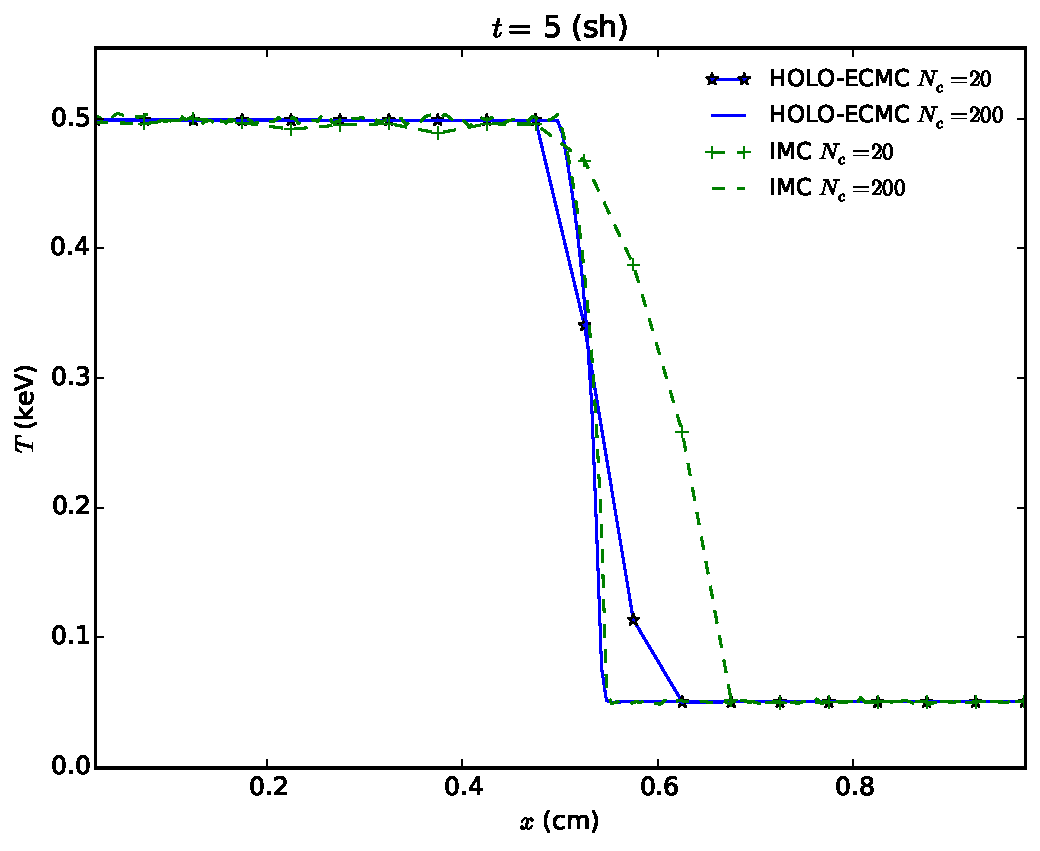
\includegraphics[width=0.99\textwidth]{two_mat_conv.pdf}
    \caption{Comparison of IMC and HOLO-ECMC.\label{twomat_full}}
\end{subfigure}    \begin{subfigure}{0.65\textwidth}
\centering
    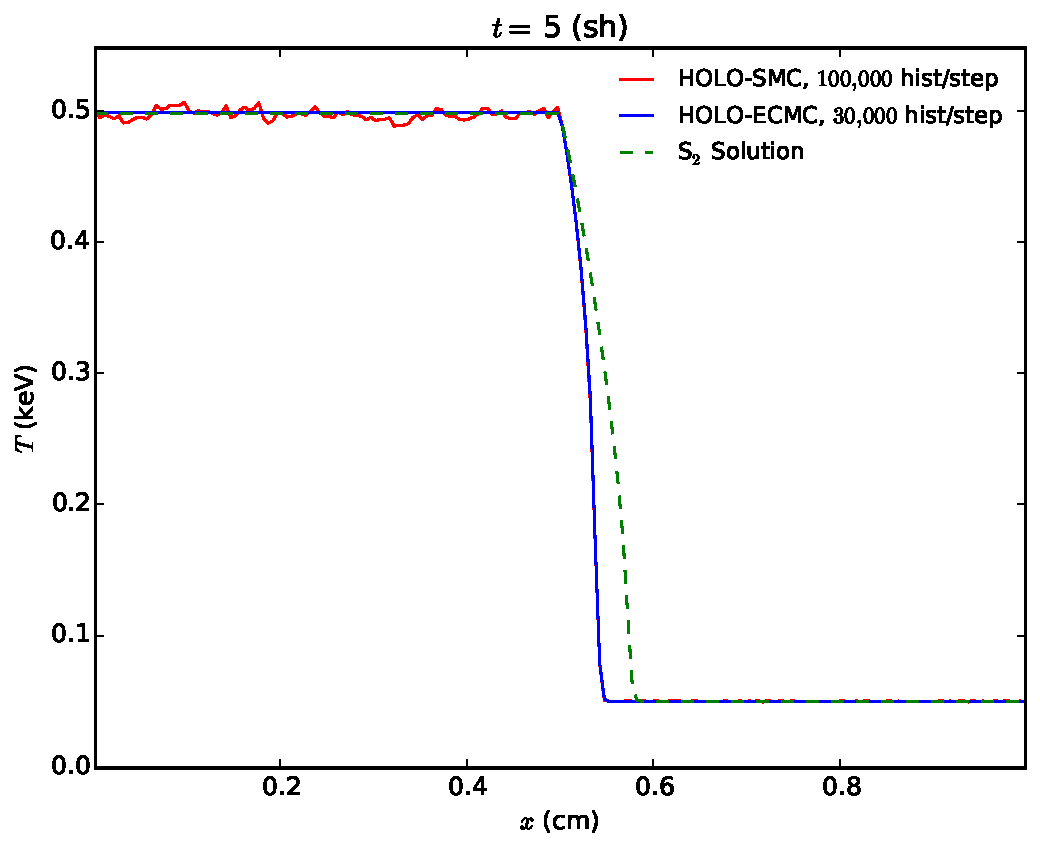
\includegraphics[width=0.99\textwidth]{two_mat_ho_compare.pdf}
    \caption{Comparison of SMC and ECMC HO solvers. \label{compare_ho}}
\end{subfigure}
    \caption{ Comparison of radiation temperatures for two material problem. \label{twomat}}
\end{figure}


\begin{table}[H]
\centering
\caption{\label{twomat_var} \textbf{Comparison of sample statistics for the
    two material problem for 200 $x$ cells.   Simulation end time is $\mathbf{t=2}$ sh.}}
\vspace{-0.1in}
\begin{tabular}{|c|cc|cc|}\cline{2-5}
    \multicolumn{1}{c|}{}       & \multicolumn{2}{|c|}{\ss} & \multicolumn{2}{|c|}{$s_{\max}$} \\ \hline
hists./step     & IMC & HOLO-ECMC  &  IMC & HOLO-ECMC   \\ \hline
   30,000	    & 3.63\%  & 0.01\% &  1      &   104,000      \\
  100,000       & 1.96\%  & 0.003\% & 1.03   &   360,000      \\ \hline
\end{tabular}
\end{table}

\subsection{Performance comparison of IMC and HOLO-ECMC}
\label{timing}

We have measured the total CPU time for simulations to provide a simplified measure of the
computational cost.  These results compare how computational times change the two
different problems and how the methods scale with time step size and particle histories.  Absolute comparisons in the computational cost of the two
methods cannot be made because the methods are implemented
in different code infrastructures. Additionally, the HOLO method fully resolves
non-linearities at each time step, whereas IMC is using a single linearized step with
lagged cross sections. Simulations were performed on the same processor, using a single CPU
core.  Reported times are the average of 10 runs and all results used 200 $x$ cells,
$\Delta t = 0.001$ sh, and an end time of $t=2$ sh.

Table~\ref{marshak_table} compares the average
simulation time per history performed for the Marshak wave problem.  The average time per history is computed by dividing the total simulation time by
the total number of histories performed (e.g., the time of the LO solves is included for
the HOLO method).  Results are given for different numbers of histories per time step, as
well as a case with an increased time step size.  The table also includes the number of LO
iterations performed per LO solve for the HOLO method, averaged over all time steps;
there are two LO solves per time step.  The same results are reported for the two
material problem in Table~\ref{twomat_table}.

The HOLO method does not scale with the number of
histories due to the fixed cost of the LO solver.  The cost of the LO solver is more
significant at the lower history counts compared to the case of $10^5$
histories, for both problems. 
There is a slight increase in the number of
newton iterations as the time step is increased, but the average cost per history is
not significantly increased.   Similar to the results
in~\cite{park}, as the time step size is increased to to 0.005 sh, the IMC method
increases in cost per time step, due to an increase in effective scattering events, particularly for the two material problem. Because
the cross sections in the the two material problem do not have a $T^{-3}$
behavior,the cost of the effective scattering cross section in IMC is more apparent,
resulting in longer simulation times. 
\begin{table}[H]
\centering
\caption{\label{marshak_table} \textbf{Comparison of average CPU times per history
    and LO iteration counts for the Marshak Wave problem. }}
\vspace{-0.1in}
	\begin{tabular}{|cc|c|cc|}\hline
hists./step & $\Delta t (sh)$ & IMC ($\mu$s/hist.) & HOLO-ECMC ($\mu$s/hist) & Newton
iters./LO solve \\ \hline
100,000                    &   0.001	& 10  &  5.3   & 3.8               \\
12,000           &   0.001	& 9.7 &	 8.1   & 4.1               \\
12,000          &   0.005	& 19  &  9.4   & 6.2                \\ \hline
\end{tabular}
\end{table}

\begin{table}[htb!]
\centering
\caption{\label{twomat_table} \textbf{Average CPU times per history and LO iteration
counts required for the two material problem.}}
	\begin{tabular}{|cc|c|cc|} \hline
hists./step & $\Delta t (sh)$ & IMC ($\mu$s/hist.) & HOLO-ECMC ($\mu$s/hist)  &
Newton iters./LO Solve\\ \hline
100,000          &   0.001	& 17  &	3.5   & 4.9 \\
30,000   &    0.001	& 18  &	6.9   &    5.0 \\
30,000    &   0.005	& 59  & 7.4   &    7.6 \\ \hline
\end{tabular}
\end{table}

\subsection{Comparison of different HO Solvers}
\label{ho_solvers}

In this section we compare the results of our HOLO algorithm with different HO
solvers for the test problems in Section~\ref{sec:marsh} and~\ref{sec:two}.  We compare standard MC (SMC) as a HO solver to the HOLO algorithm with ECMC using
both three batches and a single batch, per time step.  The use of a single batch is
similar to the approach in~\cite{rmc}.  Results are tabulated for 200 $x$ cells, using the same total
number of histories per time step, divided evenly among the batches.

Tables~\ref{homarshak_var} and~\ref{hotwomat_var} compare the results for the Marshak
wave and two material problems. The number of batches for each ECMC case is indicated
in parenthesis.  The FOM values are normalized to the reference IMC result for the
corresponding problem.  For HOLO-SMC there is
minimal reduction in variance compared to IMC in the Marshak wave problem, and the two
material problem actually demonstrates worse variance.  Sufficient histories are not
performed to accurately estimate consistency terms throughout the problem.  For ECMC,
a single batch produces less variance than the case of three equal batches.  This
indicates that if the solution cannot be resolved with the trial space (i.e., the
intensity is driven negative), a single large batch may be more accurate. It is noted
that these results only account for statistical variance, and do not account for
accuracy, which will depend on the estimates of $\epsilon$ computed each iteration.   

\begin{table}[H]
\centering
\caption{\label{homarshak_var} \textbf{Comparison of sample statistics for the Marshak Wave problem.  Number of ECMC batches is
indicated in parenthesis.}}
\vspace{-0.1in}
\begin{tabular}{|c|ccc|ccc|}\cline{2-7}
    \multicolumn{1}{c|}{}       & \multicolumn{3}{|c|}{\ss} &     \multicolumn{3}{|c|}{\FOM} \\ \hline
hists./step   & SMC & ECMC (1) & ECMC (3)  & SMC & ECMC (1) & ECMC (3)   \\ \hline
   12,000	   & 2.77\%  & 0.10\% &  0.28\% &   1.50    & 1280  & 145     \\
  100,000      & 0.98\%  & 0.03\% &  0.06\% &   1.43    & 1270  & 422     \\ \hline
\end{tabular}
\end{table}


\begin{table}[H]
\centering
\caption{\label{hotwomat_var} \textbf{Comparison of sample standard deviations for the
    two material problem. Number of ECMC batches is indicated in parenthesis.}}
\vspace{-0.1in}
\begin{tabular}{|c|ccc|ccc|}\cline{2-7}
    \multicolumn{1}{c|}{}       & \multicolumn{3}{|c|}{\ss} &
    \multicolumn{3}{|c|}{\FOM} \\ \hline
hists./step   & SMC & ECMC (1) & ECMC (3)  & SMC & ECMC (1) & ECMC
(3)   \\ \hline
   30,000	  & 5.35\%   & 0.002953\% & 0.011\%  & 0.46     & 1.51$\times10^6$   & $1.04\times10^4$          \\
  100,000     & 2.85\%   & 0.001474\% & 0.0033\% & 0.49     & 1.80$\times10^6$   & $3.59\times10^4$          \\ \hline
\end{tabular}
\end{table}

\subsection{Pre-heated Marshak wave problem and adaptive mesh refinement}

Finally, to demonstrate the potential of ECMC with adaptive space-angle mesh refinement, we perform
results for a modified Marshak wave problem. The problem is modified so that the LDFE
trial space can accurately represent the solution (i.e., the intensity is strictly
positive).  Mesh refinement is of minimal use in the previous problems due to most of
the error existing at the wavefronts, caused by the large cross sections.   The modified problem has the same material
properties and left boundary source as the Marshak wave problem in
Section~\ref{sec:marsh}.  However, the initial equilibrium
temperature and right boundary condition are raised to $0.03$ keV.   The higher initial temperature reduces the
initial cross section and increases the strength of the emission source within cells.  
The LDFE mesh can now sufficiently resolve the solution and lumping is
not required by the LO solution.  The simulation end time is 0.5 sh with a constant
time step of $\Dt=0.001$ sh.  

Fig.~\ref{hot_plot} compares the result from HOLO-ECMC with three batches and IMC.
It was found that 100 $x$ cells was sufficient to resolve the solution spatially. There is slightly more noise in IMC past the wavefront due to the increased emission
source.  Additionally, the opacity is thin enough that some photon energy is able to
reach the right boundary, in front of the wavefront. 

Table~\ref{preheat_var} compares the variances for this problem for the various HO
solvers. The FOM values are normalized to the case of HOLO-SMC with 12,000
histories per time step. The final row of the table is for an ECMC simulation with adaptive mesh
refinement (AMR).  The strategy for refinement is described in
Appendix~\ref{app:refinement}.  The adaptive
mesh refinement case used a total of nine batches, with a refinement occurring at the end
of the third and sixth batches, for every time step. The initial number of histories was adjusted so that
the average number of histories per time step is near 100,000; on average 99,881
histories per time step were used.  All ECMC meshes used 4 equally-spaced $\mu$ cells
initially. 
   The improvement in variance by ECMC compared to SMC is not as significant
as for the other problems.  This is a
result of the reduced opacity leading to intensity changing throughout the spatial
and angular domains.  The
FOM is highest for the case of ECMC with adaptive refinement. When the solution can
be resolved, the adaptive algorithm allows for a higher convergence rate of
statistical variance.  It is noted that the consistency terms and LO solution are still computed over
the fixed, coarser mesh.  However, in general, the refined mesh can produce higher accuracy in consistency terms that is
not being measured by the FOM.
\begin{figure}[htb]
  \centering
    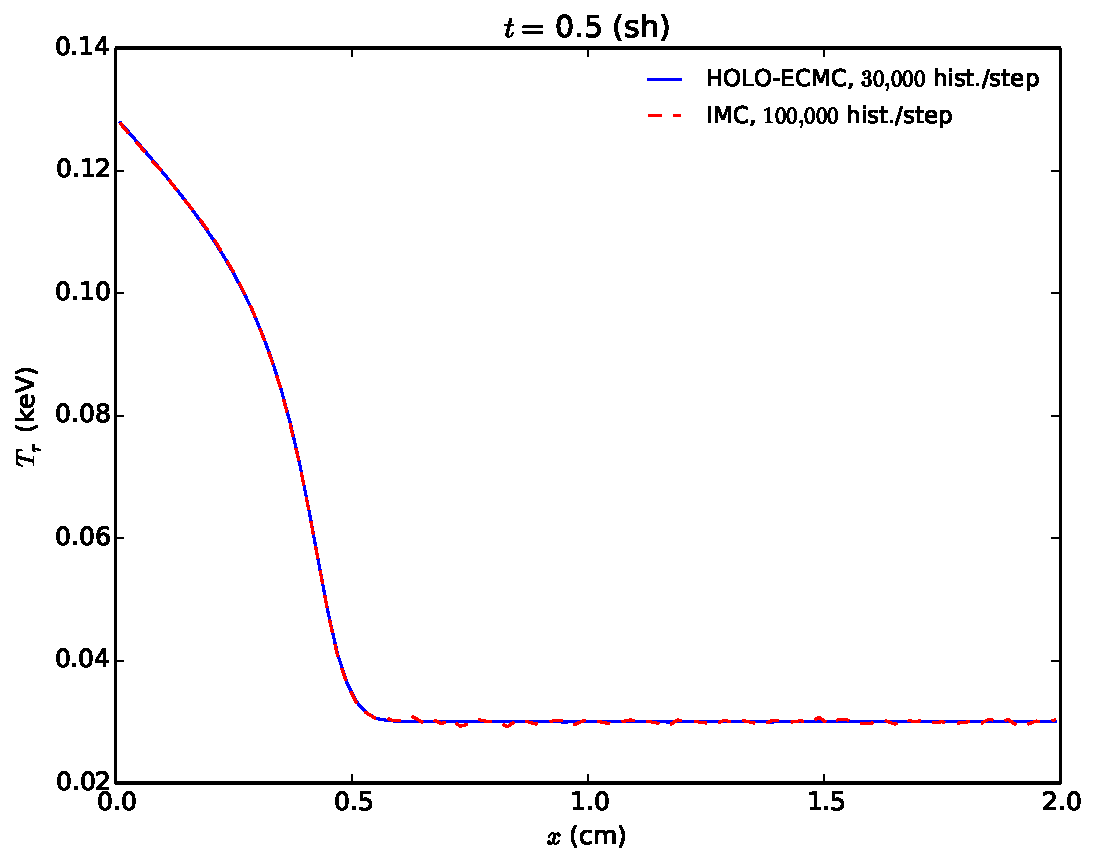
\includegraphics[width=0.65\textwidth]{heated_marshak.pdf}
    \caption{\label{hot_plot} Comparison of radiation temperatures for the pre-heated Marshak wave problem for 100
    $x$ cells at $\mathbf{t=0.5}$ sh.}
\end{figure}


\begin{table}[H]
\centering
\caption{\label{preheat_var} {Comparison of sample statistics for the 
    pre-heated marshak wave problem for 100 $x$ cells. Number of ECMC batches is
indicated in parenthesis.}}
\vspace{-0.1in}
\begin{tabular}{|c|ccc|ccc|}\cline{2-7}
    \multicolumn{1}{c|}{}       & \multicolumn{3}{|c|}{\ss} &
    \multicolumn{3}{|c|}{\FOM} \\ \hline
hists./step   & SMC & ECMC (1) & ECMC (3)  & SMC & ECMC (1) & ECMC (3)   \\ \hline
   12,000	  & 0.86\%   & 0.13\% & 0.24\% & 1      & 41  & 13      \\
  100,000     & 0.16\%   & 0.042\% & 0.08\% & 3.32   & 52  & 15       \\ 
  99,881 (AMR, 9 batches) & --  & \multicolumn{2}{c|}{ 0.038\%} & -- &
  \multicolumn{2}{c|}{61}               \\ \hline
\end{tabular}
\end{table}

\section{Accuracy in the Equilibrium Diffusion Limit}

As discussed in Sec.~\ref{sec:edl_overview}, we must ensure our method preserves the EDL.
We test a problem in the EDL by adjusting material properties to produce a strongly
diffusive domain. The EDL problem has constant cross sections with $\sigma_a=1000$
cm$^{-1}$, $\sigma_s=10$ cm$^{-1}$, $\rho c_v=6.8784\times 10^{-3}$ Jk keV$^{-1}$
cm$^{-3}$.  The domain width is 0.1 cm and 4 $\mu$ cells and 3 batches of 4,000 histories
are used for the single HO solve in all calculations. The simulation end time is 5 $sh$
and a linear increase of 15\% from $\Delta t = 0.001$ sh to a maximum $\Delta t = 0.01$ sh is used.
We compare the LDFE LO solution to a LO solution using a step discretization,
which is known to not preserve the EDL for S$_N$ equations.  The step discretization is implemented by using the scaled slope spatial
closure in Sec.~\ref{sec:spat_clos_options} with closure parameters $\gamma_i^\pm=0$ for all
cells.  

The accuracy in the equilibrium diffusion limit is compared for thefthe two spatial
discretizations, for different mesh sizes, in Fig.~\ref{fig:diff_limit}.  As demonstrated,
the LDFE spatial discretization has converged spatially, where both 20 and 200 cells
produce the same location of the wave front.  However, the step
discretization artificially propagates the energy forward; the inaccuracy is greater than
what would be expected from simply truncation error.  The step discretization will
only be accurate if the mesh cells are on the order of a mean free path, which is very large for this
problem.  Although not plotted, the material temperature overlays the radiation
temperature for the LDFE solution, in equilibrium with the radiation.

\begin{figure}
    \centering
    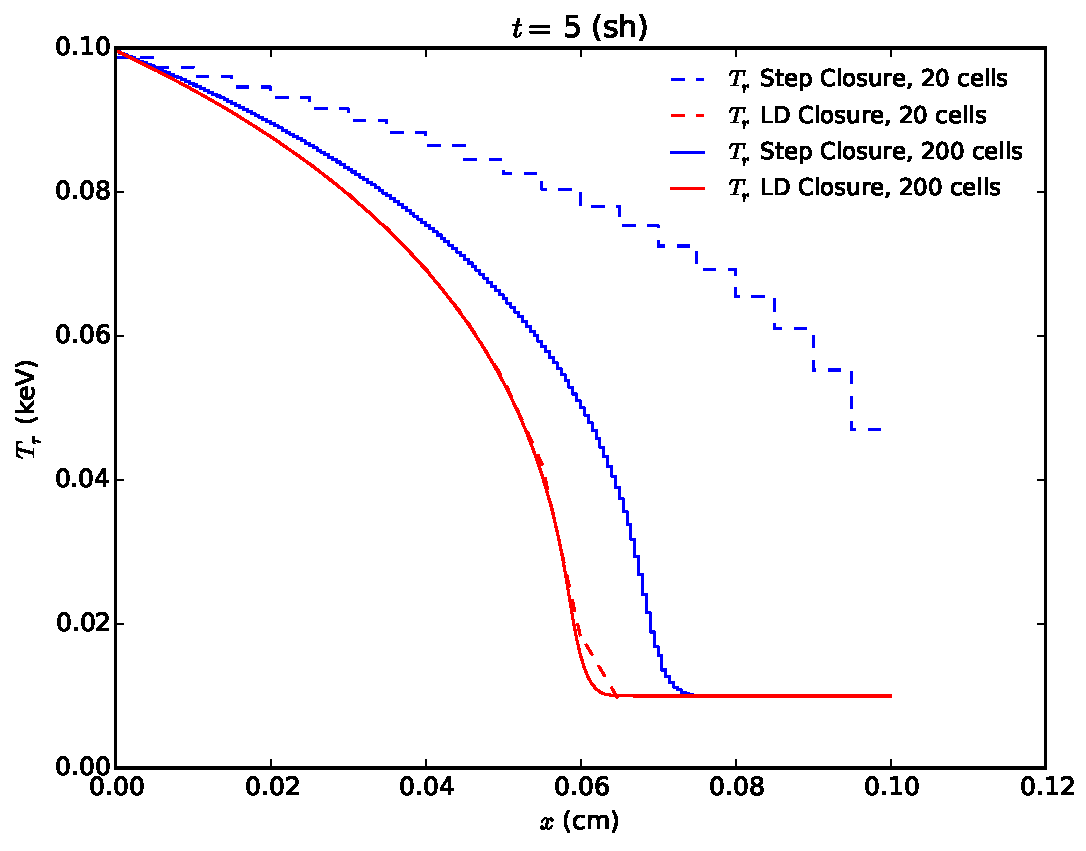
\includegraphics[width=0.6755799\textwidth]{diff_limit_compare.pdf}
    \caption{\label{fig:diff_limit}Comparison of $T_r$ for step and LDFE discretizations of the LO
equations in the equilibrium diffusion limit.}
\end{figure}



\section{Preservation of the Discrete Maximum Principle}

An important property for a discretization of the TRT equations is preservation of the
discrete maximum principle (MP).  The maximum principle states that the material temperature and mean intensity in the
interior of the domain should be bounded by the solution at the boundaries of the domain, in the
absence of interior energy sources~\cite{wollaber2013discrete,larsen_mpv}.  The analytic solution to the TRT equations satisfies a maximum
principle~\cite{larsen_mpv}, so we desire numerical approximations that preserve the MP in
a discrete sense, for each time step.
%For the discrete MP, we expect the numerical solution to be bounded by the boundary
%conditions at each time step.
For IMC simulations, violation of the maximum principle results in the material
temperature being artificially higher than the radiation temperature.  As discussed in Sec.~\ref{sec:intro}, IMC can violate the MP due to
the approximate linearization of the emission source in the time discretization; it is not
truly implicit in time.  We expect our method, with a fully implicit time discretization,
to preserve the MP with sufficient convergence of the nonlinear emission
source~\cite{larsen_mpv}.

To numerically demonstrate that our method preserves the MP, we have simulated problems
similar to those in~\cite{wollaber2013discrete}.  We modify the Marshak wave problem in
Sec.~\ref{sec:marshak???}, by decreasing $c_v$ and increasing $\sigma_a$, to produce a
problem which results in MP violations for IMC at various fixed time step sizes. 
The spatial and temporal discretization determine the occurence of MP violations for
IMC. In particular, if time steps are too large or spatial
mesh cells are too small, IMC will demonstrate MP violations~\cite{wollaber2013discrete}.  Here, we have kept the
spatial mesh size fixed and increased the time step size to produce MP violations.
The material
specifications for the problem are given in Table~\ref{tab:mpv_prob}. The domain width is 2.0 cm with
$N_c=150$ uniform spatial mesh cells.  The radiation and material energies are initially in
equilibrium at $0.01$ keV, before an isotropic boundary source of $1$ keV is applied at
the left boundary at $t=0$. The simulation end time is $t=0.1$ sh. 

The material and radiation temperature are plotted for an IMC simulation with $\Delta
t=0.025$ sh in
Figure~\ref{fig:imc_mpvrad}.  Figure~\ref{fig:imc_mpv} depicts the material temperature
for various time step sizes and the fixed mesh size of 150 cells. All IMC
simulations used 100,000 histories per time step. As demonstrated in
Fig.~\ref{fig:imc_mpvrad}, the material temperature exceeds the specified boundary
temperature and is artificially hotter than the radiation temperature.  This artificial
``temperature spike'' also leads to a slower propagation of the
wave~\cite{wollaber2013discrete}.  As shown in
Fig.~\ref{fig:imc_mpv}, as larger time-step sizes are taken the nonphysical results worsen.
It is noted that although the final solution for $\Delta t=0.0001$ sh obeys the MP, during
the first few time steps the temperature spikes are present.

The simulations are repeated with the same specifications for the HOLO method. All HOLO
simulations used a fixed mesh of 8 $\mu$ cells by 150 $x$ cells, 3 batches per time step,
and 6,000 histories per batch. A single HO solve is performed per time step, and the LO
relative convergence tolerance is $10^{-6}$. The lumping closure is used in all spatial
cells and any negativities in the HO solution are rotated to the floor value.  

As seen in
Fig.~\ref{fig:holo_mpv}, the HOLO solution does not violate the maximum principle; the
temperature is bounded from above by the radiation boundary condition.
For these simulations, it was
necessary to use the damped Newton's method discussed in Sec.~\ref{sec:damped_newton} to converge the solutions~\cite{damped_newton}. 
 A fixed damping parameter with a factor of 0.5 was found to stably converge for all
 time-step sizes that were simulated. 
Table~\ref{tab:mpv_iters} demonstrates the LO Newton iteration counts for the HOLO method.
For reference, a solution with $\Delta t = 10^{-4}$ sh is given, which required no damping
to converge.  The damped iterations require more iterations to converge.  However, it is necessary to converge the nonlinear iterations to produce
physically meaningful solutions to this problem.  The advantage of the LO solution is that
there is no additional cost for the HO solution when the damped method is used.

\begin{table}[H]
        \caption{\label{tab:mpv_prob}Problem specifications for maximum principle
        violation. Absorption cross section has form $\sigma_a = \sigma_{a,0}/T^3$.}
\centering
        \begin{tabular}{|c|c|} \hline
            $\sigma_{a,0}$ (cm$^{-1}$ keV$^3$)  & 4.0  \\ 
            $\sigma_s$ (cm$^{-1}$) & 0.0 \\
            $\rho$ (g cm$^{-3}$) & 1.0  \\
            $c_v$ (jks/keV-g) & 0.0081181  \\ \hline
        \end{tabular}
\end{table}

\begin{figure}[H]
    \centering
    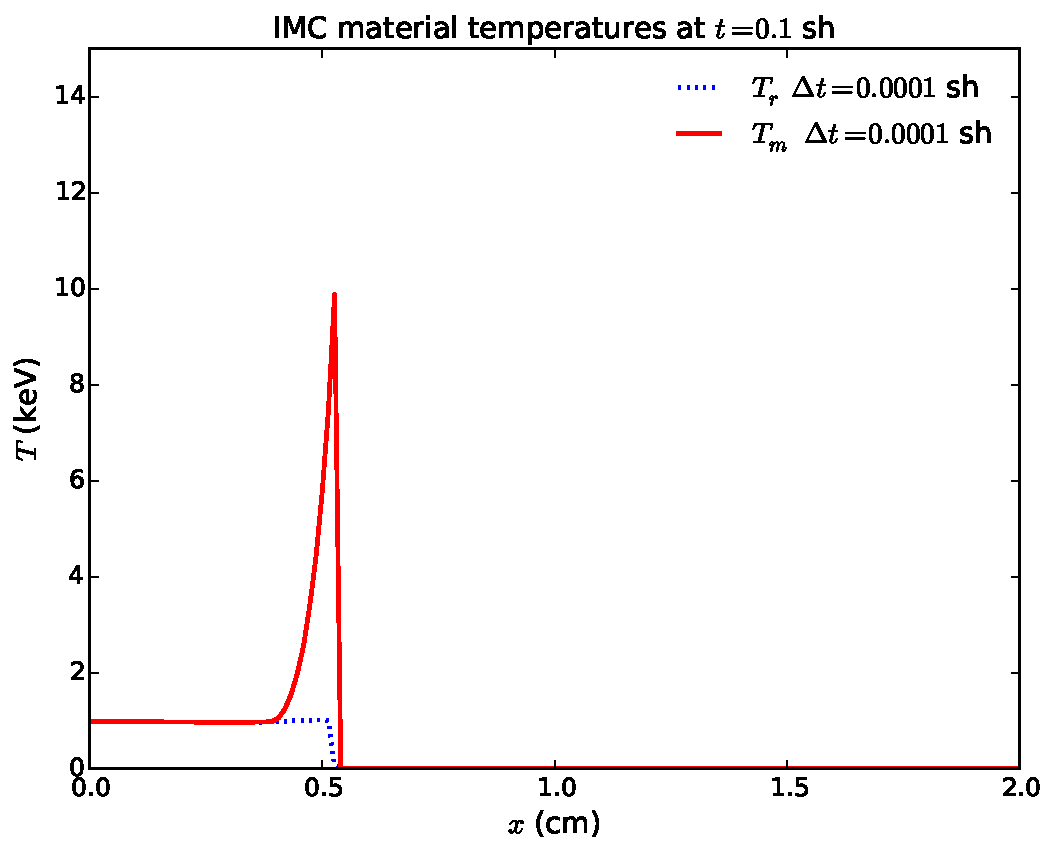
\includegraphics[width=0.6\linewidth]{mpv_rad_imc.pdf}
    \caption{\label{fig:imc_mpvrad}$T_r$ and $T$ for MP violation problem with IMC and $\Delta t = 0.001$ sh.}
\end{figure}

\begin{figure}[H]
    \centering
    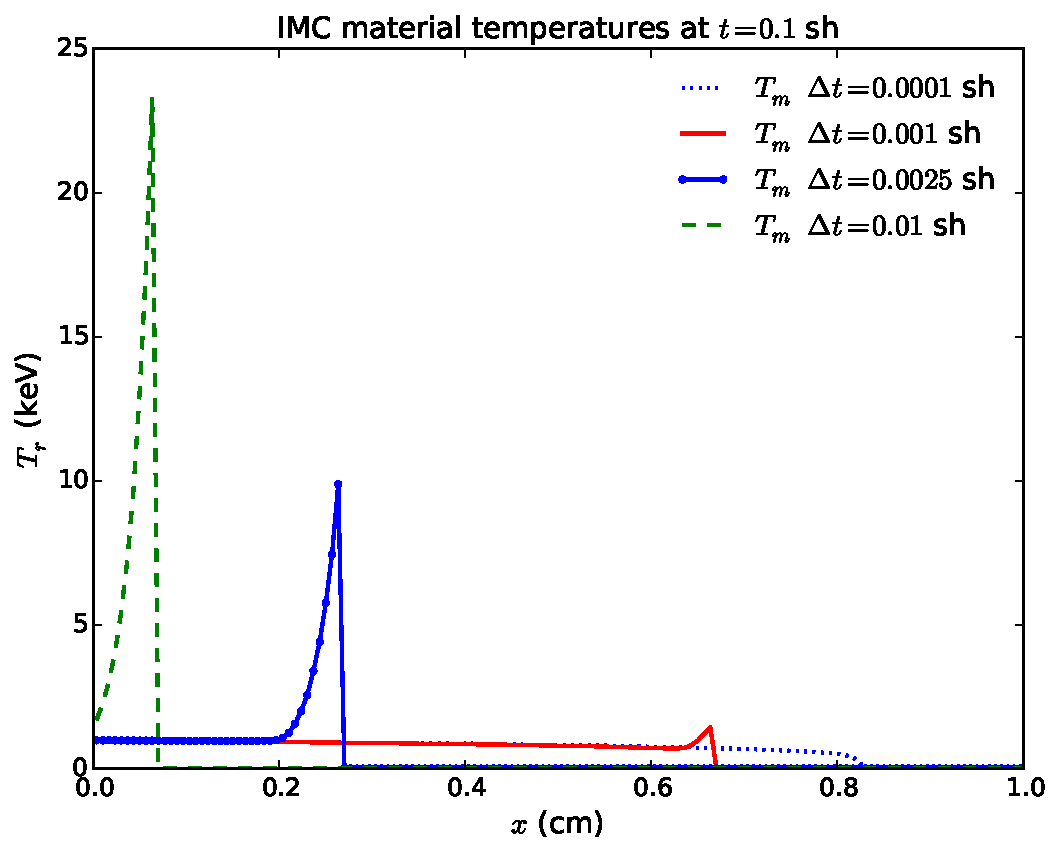
\includegraphics[width=0.6\linewidth]{mpv_mats_imc.pdf}
    \caption{\label{fig:imc_mpv}$T_m$ for MP violation problem with IMC for various time step
    sizes.}
\end{figure}

\begin{figure}[H]
    \centering
    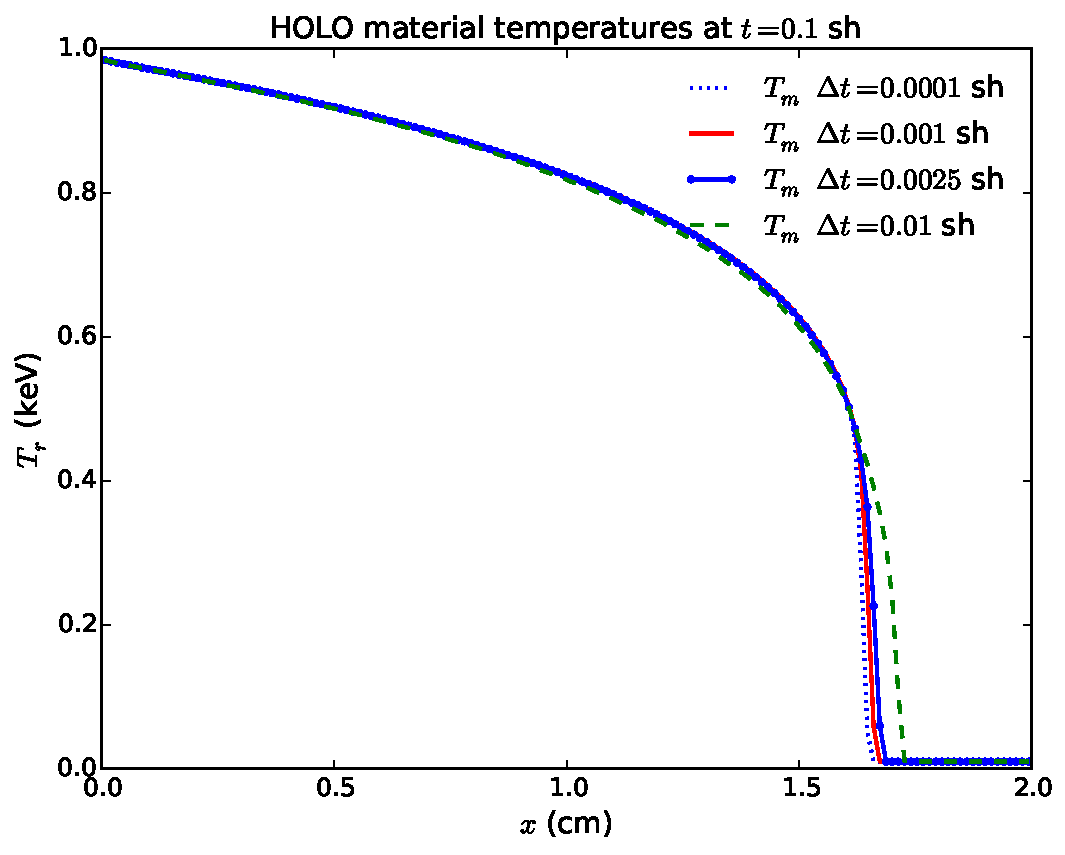
\includegraphics[width=0.6\linewidth]{mpv_mats_holo.pdf}
    \caption{\label{fig:holo_mpv}$T_m$ for MP violation problem with HOLO method for various time step
    sizes.}
\end{figure}

\begin{table}[H]
    \caption{\label{tab:mpv_iters}Comparison of LO Newton iterations for HOLO solution to 
    MP problem and different time step sizes. For $\Delta t=0.1$ sh, no damping was used; for
    all other cases a damping factor of $0.5$ was used.}  
    \centering
        \begin{tabular}{|cc|} \hline
            $\Delta t$ (sh) & Newton Iters. / LO Solve \\ \hline
            $10^{-5}$    & 3.5 \\
            $10^{-4}$    & 21.0 \\
            $10^{-3}$    & 28.5 \\
            $2.5\times10^{-3}$  & 29.7 \\
            $10^{-2}$    & 46.3 \\ \hline
        \end{tabular}
\end{table}






\chapter{\uppercase {Accelerated Iterative Solution to the LO Equations}}

As described in Sec.~\ref{sec:lo_sol}, the fully-discrete, S$_2$-like LO equations
are not easy to directly inverted efficiently in higher spatial dimensions.  
To demonstrate a possible path forward in
higher dimensions, we have investigated the use of a standard
source iteration scheme to invert the scattering terms in the LO equations.  As
material properties become more diffusive (e.g., $c_v$ is small and $\sigma_a$ is
large), the effective scattering cross sections becomes large.  This results in a spectral radius of the source iterations that approaches
unity~\cite{morel_ldtrt}.  These regimes are typical in TRT simulations, so an
acceleration method for an iterative solution is critical. 
We have accelerated the source iterations with a nearly-consistent diffusion synthetic acceleration
(DSA) method known as WLA~\cite{wla,wla_thesis}.

REWRITE: STUFF ABOUT LUMPING ETC.
We have also recast the DSA method as a preconditioner to an iterative
Krylov solution~\cite{larson_morel_sn} of the LO equations.  Generally, Krylov
methods mitigate acceleration losses due to inconsistencies in the acceleration
method.  In higher dimensions, the use of a Krylov method is necessary for effective
acceleration for nearly-consistent acceleration methods in problems with
mixed optical thicknesses~\cite{larson_morel_sn}, e.g., typical radiative transfer
problems.  Also, applying the preconditioned-Krylov approach allows for the use of
spatially lumped DSA  equations as a preconditioner, with the LO equations using
alternative fix-up methods.  We expect better acceleration performance (DID WE GET IT?) when the
LDD discretization is introduced into the LO equations. 

In the remainder of this chapter is structured as follows:  The source
iteration solution to the LO equations is detailed.  Then, the equations for the WLA DSA
method are derived and the acceleration algorithm is given.  The DSA method is then recast
as a preconditoner to a GMRES solution to the scattering iteration equations.  Finally,
results are given for a modified test problem which requires the use of acceleration.

\section{Source Iteration Solution to the Linearized LO Equations}

The linearized LO equations can be solved with a source iteration
method~\cite{lewis,morel_dsa,mcclarren_notes}.  In the source iteration
process the scattering source is lagged, which
uncouples unknowns between the two half-ranges.  This produces a lower-triangular
system where the spatial unknowns can be solve for sequentially along the two directions of flow via a
standard sweeping procedure~\cite{lewis,morel_ldtrt}.  Beginning at the left boundary, the
positive unknowns can be determined for each cell from $i=1,\ldots,N_c$.  Because the
inflow to the $i$-th cell is defined from the previous cell or boundary condition, a local system
of equations can be solved for the $\mom{\phi}_{L,i}^+$ and $\mom{\phi}_{R,i}^+$ unknowns.
The negative direction unknowns are
determined similarly, starting from the
right boundary towards the left.  The newly computed half-range
intensities can then be used to estimate the scattering source for the next iteration.  This
process is repeated until convergence.  

The source iteration process can be written in operator notation as
\begin{equation}
    \B M \psi^{l+1} = S\psi^{l} + Q,
\end{equation}
where $M$ is the discretized LO streaming plus removal operator (i.e., scattering is not
included) and $\psi$ is a vector of the half-range, FE moment unknowns.  The vector $Q$
contains the fixed source terms resulting from the linearized emission source and previous
time step moments, for each equation; the terms for the $i$-th element and the $L$ equation
are
\begin{equation}
    (\B Q)_{i,L}^\pm = \frac{\mom{\phi}_L^\pm}{c\Delta t} + \frac{1}{2}f_i \sigma_{a,i} a c \mom{
        (T^{n})^4}_{L,i}
\end{equation}
The scattering operator terms for the $i$-th element and the $L$ equations is
\begin{equation}
    (\B S \psi^l)^{\pm}_{i,L} = \frac{1}{2}\left(\sigma_{a,i} (1-f_i) + \sigma_{s,i}\right)
    \left(\mom{ \phi^l}_{i,L}^+ + \mom{ \phi^l}_{i,L}^-\right).
\end{equation}
Equivalent expressions are defined for the $R$ moment equations and boundary conditions,
forming a fully defined set of equations.

The scattering inversion must be
performed within each Newton iteration.  Thus, for the $m$-th Newton step, the source
iteration process is defined as
\begin{enumerate}
    \item Evaluate effective scattering and absorption cross sections with
        ${\{T^m_i:\;\, i=1,2,\ldots,N_c\}}$.
    \item\label{en:si_beg} Compute new scattering source $\B S \psi^l$.
    \item Perform sweeps to calculate $\psi^{l+1} = \B M^{-1} \B S\psi^{l} + \B M^{-1} Q$
    \item\label{en:si_end} If $\|\psi^{l+1} - \psi^{l} \| < $ tolerance, exit
    \item Else: repeat steps~\ref{en:si_beg}--\ref{en:si_end}.
\end{enumerate}

\section{Linear Diffusion Synthetic Acceleration}

A form of DSA referred to as the WLA method is used to accelerate the source
iterations~\cite{wla,wla_thesis}. 
Between each source iteration, a residual equation is formed that provides 
the error in the current scattering iteration. The DSA method uses an approximate,
lower-order operator to solve the error equation for a correction to the zeroth angular moment of the
intensity, i.e., the mean intensity $\phi(x)$.  The DSA equations contain a standard
finite-difference diffusion discretization that can be more efficiently
solved than the S$_2$-like equations that are being accelerated, but will accurately resolve the
slowly converging diffusive error modes.  It is important for the spatial discretization of the DSA
equations to be closely related to the discretization of the LO equations for the
acceleration to be effective and stable~\cite{adams_dsa}.  The WLA method first solves a spatially-continuous
discretization of the diffusion equation
for the iterative error on faces.  The error on the faces is then mapped onto the
volumetric moment unknowns via a LD discretization of diffusion equation~\cite{wla}.
The LD mapping resolves issues that would occur in optically-thick cells, while the
continuous diffusion equation is accurate in the EDL where acceleration is important~\cite{adams_dsa}.

In the remained of this section we derive the discretized diffusion and update equations.  To simplify notation, we
derive the diffusion equations from a generic transport equation with isotropic scattering
and source $q_0$, i.e.,
\begin{equation}\label{eq:ss_trans}
    \mu \pderiv{I}{x} + \sigma_t I = \frac{\sigma_s}{2}\left( \phi(x) + q_0\right)
\end{equation}
The WLA-DSA algorithm is then detailed.

\subsection{Forming a Continuous Diffusion Equation}

First, a continuous spatial discretization of a diffusion equation is derived.  
The mean intensity $\phi$ will ultimately be assumed continuous at faces to produce a
standard three-point finite-difference diffusion discretization. 
The zeroth and first $\mu$ moment of Eq.~\eqref{eq:ss_trans} produce the $P_1$
equations~\cite{lewis,wla_thesis}, i.e., 
\begin{align}\label{eq:dsa_bal}
    \pderiv{J}{x} + \sigma_a \phi &= q_0 \\ \label{eq:p1}
    \sigma_t J + \frac{1}{3} \pderiv{\phi}{x} &= 0, 
\end{align}
where $q_0=\int_{-1}^1 q(x,\mu) \dd \mu $.
The spatial finite element moments (defined by Eq.~\eqref{eq:x_moml} and~\eqref{x_momr})
are taken of the above equations. 
The mean intensity is assumed linear on the interior of the cell, i.e.,
$\phi(x)=\phi_Lb_L(x) + \phi_Rb_R(x)$, for $x\in(\xl,\xr)$.   Taking the left moment,
evaluating integrals, and rearranging yields
\begin{equation}
    J_{i} - J_{\il}  + \frac{\sigma_{a,i}h_i}{2} \left(\frac{2}{3} \phi_{L,i} + \frac{1}{3}
    \phi_{R,i} \right) = \frac{h_i}{2} \mom{q}_{L,i}\,\,,
\end{equation}
where $J_i$ is the average of the flux $J$ over the cell. The moments of $q$ are
not simplified to be compatible with the error equations which are in terms of moments. For the $R$ moment
\begin{equation}
    J_{i+1/2} - J_{i}  + \frac{\sigma_{a,i}h_i}{2} \left(\frac{2}{3} \phi_{L,i} + \frac{1}{3}
    \phi_{R,i} \right) = \frac{h_i}{2} \mom{q}_{R,i}\,\,.
\end{equation}
The equation for the $L$ moment is evaluated for cell $i+1$ and added to the $R$ moment
equation evaluated at $i$.  The flux $J$ is assumed continuous at $\ir$ to eliminate
the face fluxes from the equations.  The sum of the two equations becomes
\begin{multline}\label{eq:diff_noclose}
    J_{i+1} - J_{i} + \frac{\sigma_{a,i+1} h_{i+1}}{2}\left(\frac{2}{3} \phi_{L,i+1} +
    \frac{1}{3}\phi_{R,i+1}\right) + \frac{\sigma_{a,i} h_i}{2} \left( \frac{1}{3} \phi_{L,i} +
    \frac{2}{3}\phi_{R,i}\right) =\\ \frac{h}{2} \left(\mom{q}_{L,i+1} + \mom{q}_{R,i}
    \right).
\end{multline}
The mean intensity is approximated as continuous at each face, i.e., $\phi_{L,i+1} = \phi_{R,i}
\equiv \phi_{i+1/2}$.  Adding the $L$ and $R$ moments of Eq.~\eqref{eq:p1} together, with
the continuous approximation for $\phi_{i+1/2}$, produces a discrete Fick's law equation~\cite{stacy}
\begin{equation}\label{eq:ficks}
    J_{i} = -D_i \frac{\phi_{i+1/2} - \phi_{i-1/2}}{h_i},
\end{equation}
where $D_i = 1/(3\sigma_{t,i})$.
Substitution of Eq.~\eqref{eq:ficks} into Eq.~\eqref{eq:diff_noclose} and rearranging yields the following discrete diffusion
equation:
\begin{multline}
        \left(\frac{\sigma_{a,i+1} h_{i+1}}{6} -
        \frac{D_{i+1}}{h_{i+1}}\right)\phi_{i+3/2} + \left(\frac{D_{i+1}}{h_{i+1}} +
        \frac{D_{i}}{h_i} + \frac{\sigma_{a,i+1} h_{i+1}}{3} + \frac{\sigma_{a,i}
        h_{i}}{3}\right)\phi_{i+1/2} \\ + \left(\frac{\sigma_{a,i} h_{i}}{6} -
        \frac{D_{i}}{h_{i}}\right)\phi_{i-1/2} = \frac{h_{i+1}}{2} \mom{q}_{L,i+1} +
        \frac{h_{i}}{2}\mom{q}_{R,i}\;\,. 
\end{multline}
To allow for the use of lumped
or standard LD in these equations, we introduce the factor $\theta$, with
$\theta=1/3$ for standard
LD, and $\theta=1$ for lumped LD.  The diffusion equation becomes
\begin{multline}\label{eq:dsa_lumped}
    \left(\frac{\sigma_{a,i+1} h_{i+1}}{4}\left(1 - \theta\right)  -
        \frac{D_{i+1}}{h_{i+1}}\right)\phi_{i+3/2} + \left(\frac{D_{i+1}}{h_{i+1}} +
        \frac{D_{i}}{h_i} + \left(\frac{1+\theta}{2} \right)\left[\frac{\sigma_{a,i+1} h_{i+1}}{2} + \frac{\sigma_{a,i}
        h_{i}}{2}\right]\right)\phi_{i+1/2} \\ + \left(\frac{\sigma_{a,i}
        h_{i}}{4}\left(1 - \theta\right) -
        \frac{D_{i}}{h_{i}}\right)\phi_{i-1/2} = \frac{h_{i+1}}{2} \mom{q}_{L,i+1} +
        \frac{h_{i}}{2}\mom{q}_{R,i}
        \;\,. 
\end{multline}
Summation over all cells forms a system of equations for $\phi$ at each face.  

\subsubsection{Diffusion Boundary Conditions}

The upwinding in the LO system exactly satisfies the inflow boundary conditions, therefore
a vacuum boundary condition is applied to the diffusion error equations.  The equation for the left moment
at the first cell is given by
\begin{equation}\label{eq:dsa_bc}
    J_{1} - J_{1/2}  + \frac{\sigma_{a,i}h_i}{2} \left(\frac{1+\theta}{2} \phi_{L,i}
    + \frac{1-\theta}{2}
    \phi_{R,i} \right) = \frac{h_i}{2} \mom{q}_{L,i}\,\,,
\end{equation}
The Marshak boundary condition for the vacuum inflow at face $x_{1/2}$ is given as
\begin{equation}
    J^+_{1/2} = 0 = \frac{\phi_{1/2}}{4} + \frac{J_{1/2}}{2},
\end{equation}
which can be solved for $J_{1/2}$.  Substitution of the above equation and
Eq.~\eqref{eq:ficks} into Eq.~\eqref{eq:dsa_bc} gives 
\begin{equation}
    \left(\frac{1}{2}+ \sigma_{a,1}h_1\frac{1+\theta}{4} - \frac{D_1}{h_1}\right)\phi_{1/2} +
    \left( {\sigma_{a,1}{h_1}}\frac{1-\theta}{4} - \frac{D_1}{h_1}  \right)\phi_{3/2} =
    \frac{h_i}{2} \mom{q}_{L,1}
\end{equation}
A similar expression can be derived for the right-most cell.

\subsection{Mapping Solution onto LD Unknowns}

Solution of the continuous diffusion equation will provide an approximation to the error
of $\phi$ on faces, denoted as $\phi_{i+1/2}^C$. We now need
to determine the correction these results provide for the LD representation of
$\phi$. To do this, first we take the $L$ and $R$ finite element moments of the P$_1$
equations.  A LDFE dependence is assumed on the interior of the cell for $J$ and
$\phi$.  Taking moments of Eq.~\eqref{eq:dsa_bal} and simplifying yields
\begin{align}
    J_{\ir} - \frac{J_{L,i} + J_{R,i}}{2} + \frac{\sigma_{a,i} h_i}{2} \left(\frac{1}{3} \phi_{L,i} +
    \frac{2}{3}\phi_{R,i}\right) &= \frac{h_i}{2} \mom{q}_{R,i} \\
    \frac{J_{L,i} + J_{R,i}}{2} - J_{i-1/2} + \frac{\sigma_{a,i} h_i}{2}
    \left(\frac{2}{3} \phi_{L,i} +
    \frac{1}{3}\phi_{R,i}\right) &= \frac{h_i}{2} \mom{q}_{L,i}
\end{align}
The moment equations for Eq.~\eqref{eq:p1} are
\begin{align}
    \frac{1}{3}\left(\phi_{\ir} - \frac{\phi_{i,L} + \phi_{i,R}}{2}\right) +
    \frac{\sigma_{t,i} h_i}{2} \left(\frac{1}{3} J_{L,i} + \frac{2}{3}J_{R,i}\right)
    &= 0 \\
    \frac{1}{3}\left(\frac{\phi_{i,L} + \phi_{i,R}}{2} - \phi_{i-1/2} \right) +
    \frac{\sigma_{t,i} h_i}{2} \left(\frac{2}{3} J_{L,i} + \frac{1}{3}J_{R,i}\right)
    &= 0 
\end{align}
The face terms $J_{i\pm 1/2}$ and $\phi_{i\pm 1/2}$ need to be eliminated from the
system. The scalar flux is assumed to be the value provided by the continuous
diffusion solution at each face, i.e., $\phi_{i\pm1/2} = \phi_{i\pm1/2}^C$.
The fluxes are decomposed into half-range values to decouple the equations
between cells.  At $x_{\ir}$, the current is composed as $J_{i+1/2} = J_{\ir}^+ - J_{\ir}^-$,
where $+$ and $-$ denote the positive and negative
half ranges of $\mu$, respectively.  We approximate the incoming fluxes, e.g.,
$J_{i+1/2}^-$, based on $\phi_{i+1/2}^C$.  
The P$_1$ approximation provides the following relation~\cite{wla_thesis}
\begin{equation}
    \phi = 2(J^+ + J^-).
\end{equation}
At $\xr$, the above expression is solved for the incoming current $J_{i+1/2}^-$.  The
total current becomes, with $\phi_{i+1/2}=\phi_{i+1/2}^C$,
\begin{equation}\label{eq:jelim}
    J_{\ir} = J_{\ir}^+ - J_{\ir}^- = 2J_{\ir}^+ - \frac{\phi_{i+1/2}^C}{2},
\end{equation}
In the positive direction, at the right face, the
values of $\phi$ and $J$ are based on the LD representation within the cell at that
face, i.e., $\phi_{R,i}$ and $J_{R,i}$.  The standard P$_1$ approximation for the
half-range fluxes is used\cite{stacy}, i.e.,
\begin{align}
    J^{\pm} &= \frac{\gamma \phi}{2} \pm \frac{J}{2},
\end{align}
where $\gamma$ accounts for the difference between the LO parameters and the true
P$_1$ approximation. Thus, for the right face and positive half-range,
\begin{align}
    J_{\ir}^+ &= \frac{\gamma}{2}\phi_{i,R} + \frac{J_{i,R}}{2} 
\end{align}
A similar expression can be derived for $\xl$.  The total fluxes at each face are
thus
\begin{align}
    J_{i+1/2} &= \gamma\phi_{i,R} + J_{i,R} - \frac{\phi_{\ir}^C}{2} \\
    J_{i-1/2} &= \frac{\phi_{i-1/2}^C}{2} - \gamma \phi_{i,L} + J_{i,L}
\end{align}
Substitution of these results back into the LD balance equations and introduction of the
lumping notation yields the final equations 
\begin{align}
    \left(\gamma\phi_{i,R} + J_{i,R} - \frac{\phi_{\ir}^C}{2} \right) - \frac{J_{L,i} + J_{R,i}}{2} + \frac{\sigma_{a,i} h_i}{2} \left(
    \frac{(1-\theta)}{2} \phi_{L,i} +
    \frac{(1+\theta)}{2}\phi_{R,i}\right) &= \frac{h_i}{2} \mom{q}_{R,i} \\
    \frac{J_{L,i} + J_{R,i}}{2} -\left(\frac{\phi_{i-1/2}^C}{2} - \gamma \phi_{i,L} +
    J_{i,L}\right) + \frac{\sigma_{a,i} h_i}{2} \left(
    \frac{(1+\theta)}{2} \phi_{L,i} +
    \frac{(1-\theta)}{2}\phi_{R,i}\right) &= \frac{h_i}{2} \mom{q}_{L,i} 
    \\
    \frac{1}{3}\left(\phi_{i+1/2}^C - \frac{\phi_{i,L} + \phi_{i,R}}{2}\right) +
    \frac{\sigma_{t,i} h_i}{2}\left( \frac{(1-\theta)}{2} J_{L,i} +
    \frac{(1+\theta)}{2}J_{R,i}\right)    &= 0 \\
    \frac{1}{3}\left(\frac{\phi_{i,L} + \phi_{i,R}}{2} - \phi^C_{i-1/2} \right) +
    \frac{\sigma_{t,i} h_i}{2} \left( \frac{(1+\theta)}{2} J_{L,i} +
    \frac{(1-\theta)}{2}J_{R,i}\right) &= 0 .
\end{align}
The above equations are completely local to each cell and fully defined, including for
boundary cells.  The system can be solved for the desired unknowns
$\phi_{i,L}$, $\phi_{i,R}$, $J_{i,L}$, and $J_{i,R}$, which represent the mapping of
$\phi_{i+1/2}^C$ onto the LD representation for $\phi(x)$.

%\subsection{Wareing version of mapping solution onto LD Unknowns using P$_1$ incident currents}
%
%Solution of the continuous diffusion equation in the previous section provides
%correction values for $\phi$ on the faces, denoted as $\phi_{i+1/2}^C$. We now need
%to determine the correction these results provide for the LD representation of
%$\phi$. To do this, first we take the $L$ and $R$ finite element moments of the P$_1$
%equations.  A LDFE dependence is assumed on the interior of the cell for $J$ and
%$\phi$.  Taking moments of Eq.~\eqref{eq:dsa_bal} and simplifying yields
%\begin{align}
%    J_{\ir} - \frac{J_{L,i} + J_{R,i}}{2} + \frac{\sigma_{a,i} h_i}{2} \left(\frac{1}{3} \phi_{L,i} +
%    \frac{2}{3}\phi_{R,i}\right) &= \frac{h_i}{2} \mom{q}_{R,i} \\
%    \frac{J_{L,i} + J_{R,i}}{2} - J_{i-1/2} + \frac{\sigma_{a,i} h_i}{2}
%    \left(\frac{2}{3} \phi_{L,i} +
%    \frac{1}{3}\phi_{R,i}\right) &= \frac{h_i}{2} \mom{q}_{L,i}
%\end{align}
%The moment equations for Eq.~\eqref{eq:p1} are
%\begin{align}
%    \frac{1}{3}\left(\phi_{\ir} - \frac{\phi_{i,L} + \phi_{i,R}}{2}\right) +
%    \frac{\sigma_{t,i} h_i}{2} \left(\frac{1}{3} J_{L,i} + \frac{2}{3}J_{R,i}\right)
%    &= 0 \\
%    \frac{1}{3}\left(\frac{\phi_{i,L} + \phi_{i,R}}{2} - \phi_{i-1/2} \right) +
%    \frac{\sigma_{t,i} h_i}{2} \left(\frac{2}{3} J_{L,i} + \frac{1}{3}J_{R,i}\right)
%    &= 0 
%\end{align}
%The currents and fluxes on faces are decomposed into half-range values. This allows
%the cells to be decoupled by using values of $\phi_{i+1/2}^C$. 
%
%First, the definitions at face $\xr$ are considered.  The current is composed as $J_{i+1/2} = J_{\ir}^+ - J_{\ir}^-$ and the scalar flux as $\phi_{i+1/2} =
%\phi_{i+1/2}^+ + \phi_{i+1/2}^-$, where $+$ and $-$ denote the positive and negative
%half ranges of $\mu$, respectively.  The negative direction values $J_{\ir}^-$ and
%$\phi_{\ir}^-$ are upwinded from cell $i+1$. However, we approximate these values
%based on a P$_1$ expansion of the incident flux, e.g.,
%\begin{equation}
%    \psi_{\ir}^C = \frac{\phi_{\ir}^C + 3\mu J_{\ir}^C}{2}, \quad \mu<0
%\end{equation}
%We do not know $J_{\ir}^C$, but taking angular moments of the LD closure equations
%will provide enough equations to eliminate $J_{i\pm 1/2}^C$ from the system with an
%approximation.
%In the positive direction, at the right face, the
%values of $\phi$ and $J$ are based on the LD representation within the cell at that
%face, i.e., $\phi_{R,i}$ and $J_{R,i}$.  The standard P$_1$ approximation for the
%half-range currents and fluxes are used\cite{stacy}, i.e.,
%\begin{align}
%    J^{\pm} &= \frac{\gamma \phi}{2} \pm \frac{J}{2} \\
%    \phi{\pm} &= \frac{\phi}{2} \pm \frac{3J\gamma}{2}.
%\end{align}
%Thus, for the right face and positive half-range,
%\begin{align}
%    J_{\ir}^+ &= \frac{\gamma}{2}\phi_{i,R} + \frac{J_{i,R}}{2} \\
%    \phi_{\ir}^+  &= \frac{\phi_{i,R}}{2} + \frac{3\gamma}{2} J_{i,R}
%\end{align}
%The currents and partial fluxes are defined similarly for $\xl$.  Combining these
%results, equations can be formed for the face terms as
%\begin{align}
%    J_{i+1/2} &= \frac{\gamma}{2}\phi_{i,R} + \frac{J_{i,R}}{2} -
%    \left(\frac{\gamma \phi_{\ir}^C}{2} - \frac{J_{\ir}^C}{2}\right) \label{eq:jpclose} \\
%    J_{i-1/2} &= \left(\frac{\gamma \phi_{\il}^C}{2} + \frac{J_{\il}^C}{2}\right) - \left(\frac{\gamma}{2}\phi_{i,L} -
%    \frac{J_{i,L}}{2}\right) \label{eq:jlclose} \\
%    \phi_{i+1/2} &= \frac{1}{2}\phi_{i,R} + \frac{3\gamma J_{i,R}}{2} +
%    \left( \frac{\phi_{\ir}^C}{2} - \frac{3\gamma J_{\ir}^C}{2}  \right)
%    \label{eq:ppclose}  \\
%    \phi_{i-1/2} &= \frac{1}{2}\phi_{i,L} - \frac{3\gamma J_{i,L}}{2} +
%    \left(\frac{\phi_{i-1/2}^C}{2} + \frac{3 \gamma J_{\il}^C}{2}  \right)
%    \label{eq:plclose}
%\end{align}
%The lumping notation is introduced, which yields the balance equations
%\begin{align}
%    J_{\ir}^C - \frac{J_{L,i} + J_{R,i}}{2} + \frac{\sigma_{a,i} h_i}{2} \left(
%    \frac{(1-\theta)}{2} \phi_{L,i} +
%    \frac{(1+\theta)}{2}\phi_{R,i}\right) &= \frac{h_i}{2} \left(
%    \frac{(1-\theta)}{2} q_{L,i} +
%    \frac{(1+\theta)}{2}q_{R,i}\right) \\
%    \frac{J_{L,i} + J_{R,i}}{2} - J_{i-1/2}^C + \frac{\sigma_{a,i} h_i}{2}\left(
%    \frac{(1+\theta)}{2} \phi_{L,i} +
%    \frac{(1-\theta)}{2}\phi_{R,i}\right) &= \frac{h_i}{2} \left(
%    \frac{(1+\theta)}{2} q_{L,i} +
%    \frac{(1-\theta)}{2}q_{R,i}\right)      \\
%    \frac{1}{3}\left(\phi_{i+1/2}^C - \frac{\phi_{i,L} + \phi_{i,R}}{2}\right) +
%    \frac{\sigma_{t,i} h_i}{2}\left( \frac{(1-\theta)}{2} J_{L,i} +
%    \frac{(1+\theta)}{2}J_{R,i}\right)    &= 0 \\
%    \frac{1}{3}\left(\frac{\phi_{i,L} + \phi_{i,R}}{2} - \phi^C_{i-1/2} \right) +
%    \frac{\sigma_{t,i} h_i}{2} \left( \frac{(1+\theta)}{2} J_{L,i} +
%    \frac{(1-\theta)}{2}J_{R,i}\right) &= 0 .
%\end{align}
%The $q$ sources on the edges are obtained from the source moments as $q_{L,i} =
%2\mom{q}_{L,i} - \mom{q}_{R,i}$ and $q_{R,i} =
%2\mom{q}_{R,i} - \mom{q}_{L,i}$.
%Angular moments of the closure equation are manipulated to form the necessary 2 remaining equations.
%The sum of Eq.~\eqref{eq:plclose} and~\eqref{eq:ppclose} and the sum of
%Eq.~\eqref{eq:jlclose} and~\eqref{eq:jpclose} provide the two auxiliary equations,
%where we make the assumption of $J_{i+1/2}=J_{i+1/2}^C$ (this is not an
%approximation, as much as a side effect of my notation. The currents can be
%eliminated before we ever make the assumption that $\phi_{i+1/2}=\phi_{i+1/2}^C$):
%\begin{align}
%    \frac{1}{2}\left(\phi_{L,i} + \phi_{R,i}\right) + 3\gamma\left(J_{R,i} -
%    J_{L,i}\right) - 3\gamma\left(J_{i+1/2}^C - J_{i-1/2}^C\right) &=
%    \frac{1}{2}\left(\phi_{i+1/2}^C + \phi_{i-1/2}^C\right) \\
%    \frac{\gamma}{2}\left(\phi_{R,i} - \phi_{L,i}\right) + \frac{1}{2}\left(J_{R,i} +
%    J_{L,i}\right) - \frac{1}{2}\left(J_{i+1/2}^C + J_{i-1/2}^C\right) &=
%    \frac{\gamma}{2}\left( \phi_{i+1/2} - \phi_{i-1/2} \right)
%\end{align}
%These equations are completely local to each cell and fully defined.  The system can be
%solved for the desired unknowns
%$\phi_{i,L}$, $\phi_{i,R}$, $J_{i,L}$, and $J_{i,R}$, as well as the auxiliary
%unknowns $J_{i\pm 1/2}^C$.


\subsection{DSA Source Definition}

The above discretization procedure is used to determine the error in the scalar flux.
The sources $\mom{q}_{L/R}$ for the error equations remain to be defined.  They are simply the residual in
the scattering iterations, given by~\cite{lewis,morel_dsa}
\begin{equation}
    q = \sigma_s\left(\phi^{l+1/2} - \phi^{l}\right).
\end{equation}
The spatial moments are straight forward:
\begin{equation}
    \mom{q}_{L,i} = \sigma_{s,i}\left(\mom{\phi^{l+1/2}}_{L,i} -
    \mom{\phi^{l}}_{L,i}\right)
\end{equation}
The above equation is valid for lumping or standard LD.  This is because the LO
moments are defined differently for LLD or LD, resulting in equations that are
consistent.  For instance, for lumped LD, the LO system uses the spatial closure that
the edge value is defined as the moment, i.e., $\mom{\phi}_{R,i} \equiv \phi_{R,i}$.
For a standard lumped source, we desire the right equation to have $\mom{q}_{R,i} =
\sigma_s(\phi^{l+1/2}_{R,i} - \phi^{l}_{R,i})$.  Substituting the lumped closure into
the right hand side of this equation gives back the original equation, i.e., $\mom{q}_{R,i} = \sigma_{s,i}\left(\mom{\phi^{l+1/2}}_{R,i} -
    \mom{\phi^{l}}_{R,i}\right) $.  The same is true for standard LD.

\subsection{Updating the LO Unkowns}

We now have a correction to $J$ and $\phi$ for the volumetric finite element
unknowns.
Because we are interested in the time-dependent solution, we need to accelerate the solution for the
half-range fluxes, rather than just the scalar flux. We only accelerate the zeroth
moment of the angular intensity.  The error in the scalar intensities are defined as
\begin{equation}\label{eq:p1psi}
    \delta \phi^{\pm} = \frac{\delta \phi}{2} \pm \frac{3 \delta J}{4}
\end{equation}
Spatial moments are taken of $\delta \phi^{\pm}$, using the lumping notation of LD on the interior
\begin{align}
    \mom{\delta \phi^{\pm}}_L =&  \frac{1+\theta}{2}\delta \phi^{\pm}_{L} +
    \frac{1-\theta}{2}\delta \phi^{\pm}_{R}  \\
    \mom{\delta \phi^{\pm}}_R =&  \frac{1-\theta}{2}\delta \phi^{\pm}_{L} +
    \frac{1+\theta}{2}\delta \phi^{\pm}_{R}      ,
\end{align}
where Eq.~\eqref{eq:p1psi} can be used to get in terms of $\delta \phi_{L/R}$ and $\delta J_{L/R}$.

\subsection{The WLA-DSA Accelerated Source Iteration Algorithm}

We define the process of solving the diffusion like equations and mapping the error
uknowns back onto the moment equations as the operator $D^{-1}$.

The source iteration with linear DSA procedure, for the $m$-th Newton iteration, is defined as
\begin{enumerate}
    \item Evaluate effective scattering and absorption cross sections with
        ${\{T^m_i:\;\, i=1,2,\ldots,N_c\}}$.
    \item\label{en:dsa_beg} Compute new scattering source $\B S \psi^l$.
    \item Perform sweeps to calculate $\psi^{l+1/2} = \B M^{-1} \B S\psi^{l} + \B M^{-1} Q$
    \item Compute DSA residual source $\sigma_s(\phi^{l+1/2}-\phi^l)$
    \item Solve continuous DSA equations (i.e., Eq.~\eqref{eq:dsa_lumped}) for ${\{\delta \phi^{l+1/2}_{i+1/2}:\;i=0,1,\ldots,N_c\}}$
    \item Map the continuous error onto the moment unknowns.
    \item\label{en:dsa_end} If $\|\psi^{l+1} - \psi^{l} \| < $ tolerance, exit
    \item Else: repeat steps~\ref{en:dsa_beg}--\ref{en:dsa_end}.
\end{enumerate}

\section{GMRES Solution to the LO Equations}

The source iteration procedure can be recast as an iterative solution to a linear maxtrix
system.  GMRES is an effective iterative solution method for asymmetric, sparse matrix
equations~\cite{saad}.  Using the operators that have already been defined, we manipulate
the source iteration equations to form a procedure for the Krylov solution approach:
\begin{equation}
    \left(\B I  - \B M^{-1} S\right) \psi = \B M^{-1} Q,
\end{equation}
where $I$ is an identity matrix. We define combination of operators in parenthesis on the left side
of the above equation as $A$, producing a matrix equation.  Rather than form the
full matrix system, we can apply the $\B S$ and $\B M^{-1}$ operators as defined in the
previous sections.  The GMRES solution to these equations thus applies an iterative
solution technique to the above equations by repeatedly apply the operator $A$ to krylov
vectors.

To formulate the preconditioned GMRES method, we note that we want the preconditioner to approximate
the inverse of the operator on the left side of the above equation. This can be thought of
as a form of physics-based preconditioning.  Left preconditioning
was applied to the above system~\cite{saad}.  Thus in matrix form, we write the preconditioned GMRES equations as
\begin{equation}
    \left(\B I + \B D^{-1} S\right)\left(\B I - \B L^{-1} \B S \right) \psi = \left( \B I + \B
    D^{-1}\right) \B L^{-1} Q
\end{equation}
The opensource library \verb{mgmres{ is used to produce the Krylov vectors.  The
    infrastructure from the source iteration with DSA procedure can be reused to provide
    the operation of $A$ applied to the Krylov vectors returned from the GMRES solve.

Some modifications need to be made to solve these equations explicilty.  Thus, the total
algorithm for the GMRES solution is
\begin{enumerate}
    \item Evaluate effective scattering and absorption cross sections with
        ${\{T^m_i:\;\, i=1,2,\ldots,N_c\}}$.
    \item\label{en:dsa_beg} Compute new scattering source $\B S \psi^l$.
    \item Perform sweeps to calculate $\psi^{l+1/2} = \B M^{-1} \B S\psi^{l} + \B M^{-1} Q$
    \item Compute DSA residual source $\sigma_s(\phi^{l+1/2}-\phi^l)$
    \item Solve continuous DSA equations (i.e., Eq.~\eqref{eq:dsa_lumped}) for ${\{\delta \phi^{l+1/2}_{i+1/2}:\;i=0,1,\ldots,N_c\}}$
    \item Map the continuous error onto the moment unknowns.
    \item\label{en:dsa_end} If $\|\psi^{l+1} - \psi^{l} \| < $ tolerance, exit
    \item Else: repeat steps~\ref{en:dsa_beg}--\ref{en:dsa_end}.
\end{enumerate}
Without preconditioning, the diffusion solve is simply removed.


\section{Computational Results}

It is noted we are not interested in measuring the reduction of
computational time in this section because in 1D the LO equations can be directly solved efficiently.
We are just interested in ensuring that the acceleration methods can reduce the
number of scattering iterations sufficiently, including cases where inconsistencies
in the LO equations are present.

We test our acceleration methods with one simple test
problem.  This problem is a modification of the two material problem described in
Sec.~\ref{sec:two_mat}. The problem specifications are the same as before, except for
modifications to the material properties for $x>0.5$ cm.  

\subsection{Results for LD Spatial Discretization}

We first test this problem with the source iteration using DSA to accelerate and compare
to an unaccelerated SI solution.  3 batches of 10,000 particles are ran for each HO
solve, one HO solver per time step.  We tally the total number of source iterations per
time step, over the two solves.  We initialize the solution for the scattering iterations to zero at the beginning of
each LO solve. 








\section{Analytic Neutronics answer for Source fixup}

In this section we model a fixed-source, pure-absorber neutronics calculation where we know the
analytic answer to test our fixup.  If we make the mesh thick enough, we can set the
solution to be the equilibrium answer $\psi(x) = \frac{q(x)}{2\sigma_a}$. For a general
isotropic source $Q(x)$, the 1D transport equation to be solved is
\begin{equation}
    \mu \pderiv{\psi}{x} + \sigma_a \psi(x,\mu) = \frac{q(x)}{2}
\end{equation}
with boundary condition $\psi(0,\mu)=\psi_{inc}$, $\mu>0$ and
$\psi(x_R,\mu)=\frac{q(x_R)}{2\sigma_a}$ for
$\mu<0$, where $x_R$ is the right boundary.  
This first order differential equation is solved using an integration factor.
The solution to this equation for $\mu>0$ is given by
\begin{equation}
    \psi(x,\mu) = \psi_{inc}e^{\frac{-\sigma_a x}{\mu}} + \int_0^x \frac{q(x')}{2\mu}
    e^{\frac{-\sigma_a x'}{\mu}} \dd x',\quad \mu>0
\end{equation}
Integration of this result over the positive half range of $\mu$ gives
\begin{equation}
    \phi^+(x) = \psi_{inc}\E2(\sigma_a x) + \frac{1}{2}\int_0^x q(x')\E1(\sigma_a x')
    \dd x'.
\end{equation}
In the simplification of a constant source, the integral reduces to
\begin{equation}
    \phi^+(x) = \psi_{inc}\E2(\sigma_a x) + \frac{q}{2\sigma_a} \left(1 -
    \E2(\sigma_ax)\right).
\end{equation}
Also, for a constant source the solution for the negative half range becomes a constant, i.e.,
\begin{equation}
    \phi^{-}(x) = \frac{q}{\sigma_a}
\end{equation}
Combination of the above two equations gives the solution for the scalar flux:
\begin{equation}
    \phi(x) = \psi_{inc}\E2(\sigma_a x) + \frac{q}{2\sigma_a} \left(1 -
    \E2(\sigma_ax)\right) + \frac{q}{\sigma_a}.
\end{equation}


%Commands for this section
\newcommand{\dep}{\ensuremath{\delta\epsilon^{(m)}}}



\section{Face Tallies and correction near $\mu=0$}
\label{sec:face_tallies}

Face-averaged estimators of the angular error are required to compute the outflow for
estimating the spatial closure. The standard face-based
tallies~\cite{shultis_mc,favorite_faces} are used.  Tallies are weighted by
the appropriate basis functions to compute a linear FE projection in $\mu$ at each face.  The
tally score, for the angular-averaged error $\epsilon_{a,i}$ is defined as
\begin{equation}
    \hat \epsilon_{a,i\pm1/2,j} = \frac{1}{N} \sum_{m=1}^{N_{i\pm1/2,j}}
    \frac{w_m(x_{i\pm1/2},\mu)}{h_{\mu} |\mu|},
\end{equation}
where $N$ is the number of histories performed and $N_{i\pm1/2,j}$ is the number of histories
that crossed the surface $i\pm1/2$, in the $j$ angular element.   For the first
moment, the tally is
\begin{equation}\label{eq:face_mutally}
    \hat \epsilon_{\mu,i\pm1/2,j} = \frac{1}{N} \sum_{m=1}^{N_{i+1/2,j}} 
    6\left(\frac{\mu-\mu_j}{h_\mu}\right) \frac{w_m(x_{i\pm1/2},\mu)}{|\mu| h_{\mu}}.
\end{equation}
For positive and negative direction outflows are tallied
on the $x_{i+1/2}$ and $x_{i-1/2}$ faces, respectively. Particles are only tallied after leaving
a cell, and, as discussed in Section~\ref{sec:ldd_mc}, particles born on a surface do not contribute
to the tally of that surface.

Near $\mu=0$, particles can contribute large scores to the zeroth angular moment that lead to large and
unbounded variances~\cite{favorite_faces}.  To avoid large variances, we have applied the standard fixup~\cite{mcnp,favorite_faces}.  
For $|\mu|$ below some small value $\mu_{cut}$, 
particles contribute the expected score over the range $(0,|\mu_{cut}|)$, based on an
approximate, isotropic particle density. Thus, scores in this range have no variance.  Assuming
an isotropic particle density $I_0$, the average of
$1/\mu$, for positive $\mu$, is
\begin{equation}
    \overline{1/\mu} = \frac{\displaystyle \int_0^{\mu_{cut}}\frac{1}{\mu} I_0 \,\dd
\mu}{\displaystyle \int_0^{\mu_{cut}} I_0\, \dd \mu} =
    \frac{2}{\mu_{cut}}.
\end{equation}
For negative $\mu$, $\overline{1/\mu}=-2/\mu_{cut}$.
All particles in the range $(0,|\mu_{cut}|)$ contribute the expected score by evaluating
the tallies at $\pm\mu = \pm2/\mu_{cut}$.  It is noted that the first angular moment tallies are
well defined because there is no $\mu$ term in the tally. THIS ISNT REALLY TRUE NOW
BECAUSE THE FINITE ELEMENT FIRST MOMENT IS FINE. Additionally, assuming an isotropic intensity over the range helps to limit
the first moment near $\mu=0$, which the LD trial space
generally cannot resolve anyways, as discussed in ???.

\section{MC solution with LDD trial space}
\label{sec:ldd_mc}

The inclusion of the outflow discontinuity has a minimal effect on the treatment of the
residual source. The residual source and process of estimating moments of
the error on the interior of a space-angle cell is unchanged.  The process of estimating
the solution on the outgoing face requires tallying the solution when particles leave a
cell. The tallying process is discussed later in Section~\ref{sec:face_tallies}.  

Applying $L$ to the LDD trial space, as shown in Fig.~\ref{fig:ldd}, results in two $\delta$ functions at each interior face.
For positive flow, at a face $x_{i+1/2}$, the face portion of the residual is defined as
\begin{align}
    \label{eq:res_face}
    \rface(x_{i+1/2}) &= -\mu \pderiv{\tilde I^{(m)}}{x}\big|_{x_{i+1/2}}\\
    &= \rface(x_{i+1/2}^-)\delta^-(x - x_{i+1/2}) + \rface(x_{i+1/2}^+)\delta^+(x - x_{i+1/2}) 
\end{align}
where
\begin{align}
    \rface(x_{i+1/2}^-) &= -\mu\left( \tilde I^{(m)}(x_{i+1/2},\mu) - \tilde I^{(m)}(x_{i+1/2}^-,\mu)
           \right)\\
    \rface(x_{i+1/2}^+) &= -\mu\left( \tilde I^{(m)}(x_{i+1/2}^+,\mu) -
           \tilde I^{(m)}(x_{i+1/2},\mu)
           \right).
\end{align}
Here, $I^{(m)}(x_{i+1/2}^+)$ and $I^{(m)}(x_{i+1/2}^-)$ are the LD solution extrapolated to $x_{i+1/2}$ from the
$x$ cell $i$ and cell $i+1$, respectively.
Particles sampled from the two $\delta$-functions have the same starting location.  The
only difference is, for positive $\mu$,  particles sampled from $\rface(x^-_{i+1/2})$ will
contribute to the face tally at $x_{i+1/2}$; the opposite is true for negative $\mu$.

To reduce variance, we do not sample the two $\delta$ functions independently.
%or score contributions to the outflow face from the interior face source. 
Instead, we combine the
two $\delta$-functions into a single face source,
do not score particles at the face from which they are sampled.  To account for the
untallied error, we add the analytic
contribution to the error from the face source to the corresponding face at the end of a batch.
It is noted the combination of the two $\delta$-functions produces the same residual source as the
original LD residual.

Define the additional error contribution 
from the face sources at $x_{i+1/2}$ as $\dep$.  This additional error is tallied
everywhere by MC, except for at $x_{i+1/2}$.  The transport equation satisfied by $\dep$, for positive
$\mu$, with effective total cross 
section $\hat \sigma_t$, is
\begin{equation}
    \label{eq:ho_face}
    \mu \pderiv{\dep}{x} + \hat\sigma_t \dep = \rface(x_{i+1/2}^-)\delta^-(x - x_{i+1/2}) + \rface(x_{i+1/2}^+)\delta^+(x - x_{i+1/2}) 
\end{equation}
This equation is integrated from $x_{i+1/2}-\alpha$ to $x_{i+1/2}$ to produce
\begin{multline}
    \mu\dep(x_{i+1/2},\mu) - \mu\dep(x_{i+1/2}-\alpha,\mu)  + \int\limits_{x_{i+1/2}-\alpha}^0 
    \hat \sigma_t \dep \dd x  \\ =  \rface(x_{i+1/2}^-) +
        \int\limits_{x_{i+1/2}-\alpha}^0\rface(x_{i+1/2}^+)\delta^+(x - x_{i+1/2}) \dd x.
\end{multline}
The integral on the right side of the equation is zero because $\delta^+(x-x_{i+1/2})$ is
zero for $(-\infty,x_{i+1/2}]$.  The limit of the above equation is taken as $\alpha\to0$, i.e.,
\begin{multline}
    \lim_{\alpha\to0}\left( \mu\dep(x_{i+1/2},\mu) - \mu\dep(x_{i+1/2}-\alpha,\mu)  + \int\limits_{x_{i+1/2}-\alpha}^0 
    \hat \sigma_t \dep \dd x \right)  = \lim_{\alpha\to0} \rface(x_{i+1/2}^-) 
\end{multline}
The integral goes to zero because $\dep$ is smooth on the interior of the cell, and
$\mu\dep(x_{i+1/2}-\alpha,\mu)$ goes to zero because there is no source upstream of
$x_{i+1/2}^-$. Thus, the final solution is
\begin{equation}
    \dep(x_{i+1/2},\mu) = \frac{\rface(x_{i+1/2}^-)}{\mu} = 
     \tilde I^{(m)}(x_{i+1/2}^-,\mu) - \tilde I^{(m)}(x_{i+1/2},\mu)
.
\end{equation}
The update for $I(x_{i+1/2},\mu)$ is 
\begin{align}
   \tilde I^{(m+1)}(x_{i+1/2},\mu) &= \tilde I^{(m)}(x_{i+1/2},\mu) + \epsilon^{(m)}(x_{i+1/2},\mu) +
    \dep(x_{i+1/2},\mu) \\ 
        &= \tilde I^{(m)}(x_{i+1/2}^-,\mu) + \epsilon^{(m)}(x_{i+1/2},\mu).
\end{align}
This result has the peculiar effect that the estimation of the solution on a face depends only on
the interior solution $\tilde I^{(m)}(x_{i+1/2}^-,\mu)$ and not the previous face value 
$\tilde I^{(m)}(x_{i+1/2},\mu)$. This could be used to only estimate
face values in particular cells, at any chosen batch.



\section{Implementation of ECMC finite-element space, tallies, and residual sampling}

\label{app:tallies}

The ECMC solver uses a finite element representation in space and angle. On the
interior of the cell with the $i$-th spatial index and $j$-th angular index, the linear representation is defined as
\begin{equation*}
    \tilde I(x,\mu) = I_{a,ij} + \frac{2}{h_x}I_{x,ij}\left(x-x_i\right) +
    \frac{2}{h_\mu}I_{\mu,ij}\left(\mu-\mu_j\right), \quad x_\il <  x < x_\ir,\quad
     \mu_\jl \leq \mu \leq \mu_\jr
\end{equation*}
The spatial cell width is $h_x$, the angular width is
$h_\mu$, the center of the cell is $(x_i,\mu_j)$, and
\begin{align}\label{app1}
    I_{a,ij} &= \frac{1}{h_x h_\mu} \iint\limits_{\mathcal{D}} I(x,\mu)\, \dd x \dd \mu \\
    I_{x,ij} &= \frac{6}{h_xh_\mu}\iint\limits_{\mathcal{D}} \left(\frac{x - x_i}{h_{x}}\right)
    I(x,\mu)\, \dd x \dd \mu \\ \label{app2}
    I_{\mu,ij} &= \frac{6}{h_xh_\mu}\iint\limits_{\mathcal{D}}
     \left(\frac{\mu - \mu_j}{h_{\mu}}\right)
    I(x,\mu)\, \dd x \dd \mu,
\end{align}
where $\mathcal{D}: x_\il \leq  x \leq  x_\ir \times \mu_\jl \leq \mu \leq \mu_\jr$.
%$I_a$ is the cell average intensity, and $I_\mu$ and $I_x$ define the
%the first moment in $\mu$ and $x$ of the intensity, respectively. 
Standard upwinding in space is used to
define $I(\mu)$ on incoming faces. 

This representation can directly be plugged into
Eq.~\eqref{eq:resid} and evaluated to produce the residual source in the ECMC HO transport
problem.  The MC source $r^{(m)}(x,\mu)$ in Eq.~\eqref{eq:mc_err}
consists of both face and volumetric sources and can produce positive and
negative weight particles.  The distribution for sampling particle coordinates, in space and angle, is based on the $L_1$
norm over space and angle of the residual~\cite{jake}.  A particular cell volume or face 
is sampled, and then rejection sampling~\cite{shultis_mc} is used to sample from
the appropriate distribution on the face or interior of the space-angle cell.  If the
residual is negative at the sampled coordinates, the weight of the particle history is negative.

During a MC batch, moments of the error are tallied.  The necessary moments of the error are
defined analogously to Eq.'s~\eqref{app1}--\eqref{app2}.
The tallies are evaluated by weighting the particle density with the appropriate
basis function and integrating along the history path through the cell.  For the cell average, the $n$-th
particle makes the contribution
\begin{equation}
   \epsilon^n_{a,ij} = \frac{1}{h_xh_\mu} \int\limits_{s^n_o}^{s^n_f}  w^n(x,\mu) \dd s,
\end{equation}
where $s_o^n$ and $s_f^n$ are the beginning and end of the $n$-th particle track in the cell and $w(x,\mu)$ is
the weight of the error particle in the MC simulation.  Weight is attenuated exponentially, i.e., $w(x,\mu)\propto
\exp(-\sigma_t|x/\mu|)$.
Substitution of the exponential attenuation of the weight produces the result
\begin{equation}
    \epsilon^n_{a,ij} = \frac{w(x_0,\mu)}{\sigma_t h_x h_\mu} \left(1 -
    e^{-\sigma_ts^n}\right).
\end{equation}
Here, $w(x_0,\mu)$ is the particle weight at the start of the path and $s^n$ is the
length of the track. The contribution of a
particle track to $\epsilon_x$ is given by
\begin{equation}
    \epsilon^n_{x,ij} = \frac{w(x_0,\mu)}{h_x^2h_\mu \sigma_t} \left[x_0 - x_f e^{-\sigma_t s^n}
        + \left(\frac{\mu}{\sigma_t} - x_i \right)\left(1-e^{-\sigma_t s^n}\right),
    \right]
\end{equation}
where $x_0$ and $x_f$ are the beginning and ending $x$ coordinates of the $n$-th
path.  The contribution to the first moment in $\mu$ is 
\begin{equation}
    \epsilon^n_{\mu,ij} = \frac{w(x_0,\mu)}{h_{\mu}^2h_x\sigma_t}\left(\mu -
    \mu_j\right) \left(1 - e^{-\sigma_ts^n}\right),
\end{equation}
where the particle $x$-direction cosine $\mu$ does not change because it is a pure-absorber simulation.
Finally, the moments of the error are simply the average contribution of all particles.

\section{Adaptive Mesh Refinement}
\label{app:refinement}
This section describes the adaptive refinement strategy for the ECMC algorithm.
Detailed equations for performing projections between meshes and computing the residual source on
the refined meshes can be found in~\cite{jake}.  At the end of the ECMC batch,
refinement is performed in space-angle cells based on a jump indicator.  The jump
indicator is the magnitude of the different between $I(x,\mu)$ in adjacent cells,
averaged over each edge.  The value of the largest jump, out of the four edges within a
cell, is used as the
indicator for that cell.  Based on this indicator, the 20\% of cells with the largest jump are
refined.  Future work will explore simply using $\epsilon$ to indicate refinement,
rather than the jump error.  The refinement of a cell is chosen to be symmetric, with each space-angle cell divided into four
equal-sized cells.  The solution for $\tilde{I}^{n+1}(x,\mu)$ of the batch is projected onto
the finer mesh for the next batch. Because the dimensionality of the sample space has
increased, we increase the number of histories per batch s.t. the ratio of the number
of histories to total cells is approximately constant for all meshes.  At the end of the last HO solve in a time step,
$\tilde{I}^{n+1}$ is projected back onto the original, coarsest mesh and stored as
$\tilde{I}^{n}$ for the next time step.


\section{Spatial Closure based on the HO Solution}
\label{sec:spat_clos}

This sections describes an alternative spatial closure to the LO equations based on 
a parametric relation from the HO solution. In addition to estimating the angular
consistency terms, the HO intensity estimates a relation between volume and face-averaged
intensities to eliminate the remaining unknowns from the equations.  In the remainder of
this section, we will motivate the HO spatial closure by manipulating a half-range balance
equations to form a single unknown for each cell and half range.  We will then discuss
the forms of HO spatial closures investigated, based on modifications to standard spatial closures.

\subsection{Motivation}

A half-range balance equation for $\mu>0$ is formed by adding the
exact $L$ and
$R$ radiation moment equations given by
Eq.~\eqref{eq:exact_lmomp}~and~\eqref{eq:exact_rmomp}, i.e.,
\begin{equation}\label{eq:hr_bal}
    \mu^+_{i+1/2}\phi_{i+1/2}^+ - \mu^+_{i-1/2}\phi_{i-1/2}^+ +
    {\sigma_{a,i}h_i} \phi_i^+ = \frac{h_i}{2} q_i,
\end{equation}
where $q_i$ represents the cell-averaged emission source.  In the HOLO algorithm, after
estimating the consistency terms $\mu_{i\pm1/2}^+$ upwinding the inflow term
$\phi_{i-1/2}^+$, an additional equation is needed to eliminate the outflow $\phi_{i+1/2}^+$ to produce an
equation for a single unknown $\phi_{i}^+$.  Standard spatial discretizations techniques
use a fixed approximation for all cells to eliminate the outflow in terms of other
unknowns.  Alternatively, the HO solution can be used to estimate a parametric relation
between the other unknowns and the outflow, i.e.,
\begin{equation}\label{eq:ho_clos}
    \phi_{i+1/2}^+ = f(\gamma^{+,HO}_i, \phi_i^+, \phi_{x,i}^+, \phi_{i-1/2}^+),
\end{equation}
where $\gamma^{HO,+}_i$ is a local constant to be estimated with the HO solution and $f$ is some
function of some number of the input
variables.  The ECMC solution can provide all of the unknowns in the above equation, so
the value of $\gamma^{HO}_i$ can be determined directly. 

If the problem were linear, or the nonlinear problem was fully converged,
then application of this closure can ensure that the HO and LO equations produce the same
moments, preserving the HO accuracy.  To produce the
same moments, the HO solution must also satisfy the local balance equation, e.g.,
Eq.~\eqref{eq:hr_bal}.  Then the LO equations and HO equations must have the same moments
to satisfy both Eq.~\eqref{eq:ho_clos} and Eq.~\eqref{eq:hr_bal}, upon nonlinear
convergence of the outer HOLO iterations. If any higher moments are introduced through the spatial closure,
then the HO solution must also satisfy the corresponding balance equations that the LO
equations do.  For example, both the LO and HO equation must satisfy the
first moment equation in space if the closure is a function of the first moment.  

As TRT problems are non-linear (i.e., scattering or thermal emission are included in
$q$), the moments will only be preserved upon non-linear convergence of the source.  The
nonlinearity introduces the possibility for stability
issues, particularly with MC noise.  However, we have already consistently formed angular consistency terms, so the
the spatial closure should be more stable than introducing other terms, such as
in NDA methods~\cite{rmc,willert}. 





\subsection{Choice of Spatial Closure}
\label{sec:spat_clos_options}

We will
explore two different closure relations based on modifications to the standard LD closure: a scaled slope, i.e.,
\begin{equation}\label{eq:cl_slope1}
    \phi_{i\pm1/2}^\pm = \phi_i^+ \pm \gamma_i^{\pm} \phi_{x,i}^+
\end{equation}
and a scaled average
\begin{equation}\label{eq:cl_avg1}
    \phi_{i\pm1/2}^\pm = \gamma_i^{\pm} \phi_i^+ \pm \phi_{x,i}^+,
\end{equation}
where a value of $\gamma_i = 1$ produces the standard linear discontinuous expressions for
the extrapolated outflows.  Our LO system is formulated in terms of $L$ and $R$ moments, rather than the average and
slope.  Thus, Eq.~\eqref{eq:cl_slope1} and~\eqref{eq:cl_avg1} are expressed in terms of the $L$ and $R$
unknowns, using the relations given in App.~\ref{app:lo_mom_relations}.  In terms of these
moments, the scaled-slope closure is
\begin{align}\label{eq:cl_slope}
    \phi_{i+1/2}^+  &= \left(\frac{\ds 1 - 3 \gamma_i^+}{\ds 2 }  \right)
    \mom{\phi}_{L,i}^+ + \left(\frac{\ds 1 + 3 \gamma_i^+}{\ds 2 }  \right)
    \mom{\phi}_{R,i}^+ \\
    \phi_{i-1/2}^-  &= \left(\frac{\ds 1 + 3 \gamma_i^-}{\ds 2 }  \right)
    \mom{\phi}_{L,i}^- + \left(\frac{\ds 1 - 3 \gamma_i^-}{\ds 2 }  \right)
    \mom{\phi}_{R,i}^- 
\end{align}
and the scaled-average relation is
\begin{align}\label{eq:cl_avg}
    \phi_{i+1/2}^+  &= \left(\frac{\ds  \gamma_i^+ - 3}{\ds 2 }  \right)
    \mom{\phi}_{L,i}^+ + \left(\frac{\ds \gamma_i^+ + 3}{\ds 2 }  \right)
    \mom{\phi}_{R,i}^+ \\
    \phi_{i-1/2}^-  &= \left(\frac{\ds \gamma_i^- + 3}{\ds 2 }  \right)
    \mom{\phi}_{L,i}^- + \left(\frac{\ds \gamma_i^- - 3}{\ds 2 }  \right)
    \mom{\phi}_{R,i}^- .
\end{align}

The HO solution is used to estimate $\gamma_i$. The MC solution must be modified
to tally the MC estimated intensity on faces. For example, for $\mu>0$, the LO equations for
moments at $k+1$ use closure parameters evaluated at $k+1/2$ as
\begin{equation}
    \gamma_i^{+,HO,k+1/2} = \frac{\phi_{i+1/2}^{+,HO,k+1/2} -
    \phi_{i}^{+,HO,k+1/2}}{\phi_{x,i}^{+,HO,k+1/2}},
\end{equation}
for the scaled-slope closure.  For this closure, as the slope goes to zero this expression
becomes undefined.  In cells where the slope is $O(10^{-13} \psi_i)$, we use $\gamma_i=1$.
For the problems tested, no issues have occurred with this closure, even $\gamma$
can become very large for common, small values of $|\psi^x/\psi_i|$.  This is because in
such regions the solution is changing minimally anyways. 
The main benefit of the scaled-slope closure is it allows for values of $\gamma$ that are
equivalent to other closures, as discussed in App.~\ref{app:lo_mom_relations}:
$\gamma_i=0$ produces a step closure~\cite{larsen_edl}, which has a zero slope over the cell, and $\gamma_i=1/3$
produces a lumping-equivalent closure. 

\subsection{The Doubly-Discontinuous Trial Space}

Because of the temperature unknowns and the HO scattering source representation, a
representation on the interior of the cell for the temperature and intensity is needed.
Thus, we introduce a linear doubly discontinuous (LDD) trial space
for the half-range intensities, which is depicted in Fig.~\ref{fig:ldd_space}.  The linear
relation on the interior of the cell preserves the $L$ and $R$ moments of the solution,
and the outflow from the cell is some parametric (i.e., non linear) extrapolation of
those moments. 
The temperature is still represented with a linear interpolant of $T^4$ and $T$.  This
trial space has an extra unknown in the radiation equations for each cell and direction, which is eliminated
from the system with the HO spatial closure.  The ECMC algorithm is modified to also
include a LDD trial space which allows for estimate of the solution at faces, as discussed
later in Sec~\ref{sec:ldd_mc}. 

To solve the LO equations, Eq.~\eqref{eq:cl_slope} or~\eqref{eq:cl_avg} is substituted
locally for
the appropriate outflow face term in each LO moment equation. There is a spatial closure parameter for each
half-range, for each cell.
 The $\gamma_i^\pm$ are
estimated from the previous HO solution. For the initial LO solve within each
time step, the outflow is assumed continuous, using the standard upwinding and LD closure.  
As an example, the positive half-range and $L$ moment equation (i.e.,
Eq.~\eqref{eq:exact_lmomp}), for the scaled-slope closure, becomes
\begin{multline}
    -2{\mu}_{i-1/2}^{n+1,+} \left[\left(\frac{\ds 1 - 3 \gamma_{i-1}^{HO,+}}{\ds 2 }  \right)
        \mom{\phi}_{L,i-1}^+ + \left(\frac{\ds 1 + 3 \gamma_{i-1}^{HO,+}}{\ds 2 }  \right)
    \mom{\phi}_{R,i-1}^+
    \right] \\ + \cur {\mu}_{L,i}^{n+1,+}
  \mom{\phi}_{L,i}^{n+1,+}
  +  \cur\mu_{R,i}^{n+1,+}
  \mom{\phi}_{R,i}^{n+1,+}\\ +  \left(\sigma_{t,i}^{n+1}+\frac{1}{c \Delta t} \right) h_i 
  \mom{\phi}_{L,i}^{n+1,+} -  \frac{\sigma_{s,i} h_i}{2} \left( \mom{\phi}_{L,i}^{n+1,+} +
  \mom\phi_{L,i}^{n+1,-}\right)\\  = \frac{h_i}{2} \mom{\sigma_a^{n+1} a c T^{n+1,4}}_{L,i} +
  \frac{h_i}{c\Delta t}\mom{\phi}_{L,i}^{n,+},
    \label{eqn:clsd_posl}
\end{multline}
and the $R$ moment equation becomes
\begin{multline}
    2{\mu}_{i+1/2}^{n+1,+} \left[
    \left(\frac{\ds 1 - 3 \gamma_{i}^{HO,+}}{\ds 2 }  \right)
        \mom{\phi}_{L,i}^+ + \left(\frac{\ds 1 + 3 \gamma_{i}^{HO,+}}{\ds 2 }  \right)
    \mom{\phi}_{R,i}^+
    \right]  \\ 
    - \cur {\mu}_{L,i}^{n+1,+}
  \mom{\phi}_{L,i}^{n+1,+}
  -  \cur\mu_{R,i}^{n+1,+}
  \mom{\phi}_{R,i}^{n+1,+} +  \left(\sigma_{t,i}^{n+1}+\frac{1}{c \Delta t} \right) h_i 
  \mom{\phi}_{R,i}^{n+1,+} \\-  \frac{\sigma_{s,i} h_i}{2} \left( \mom{\phi}_{R,i}^{n+1,+} +
  \mom\phi_{R,i}^{n+1,-}\right) = \frac{h_i}{2} \mom{\sigma_a^{n+1} a c T^{n+1,4}}_{R,i} +
  \frac{h_i}{c\Delta t}\mom{\phi}_{R,i}^{n,+}.
    \label{eqn:clsd_posr}
\end{multline}
These equations contain only the original desired radiation moment and LD temperature unknowns.
During the Newton solve, once new half-range
intensities are determined, the temperatures are updated using the same material
energy equations as for the LD closure, i.e., Eq.~\eqref{eq:lo_mat_dis1} and Eq.~\eqref{eq:lo_mat_dis2}.

Because the
outflow from one cell is upwinded into the next cell, energy conservation by the LO
equations is preserved.
The closed equations have the
same numerical complexity as the LDFE LO equations, but with an increased storage on the
coarse mesh for the
$\{\gamma_i\}$.  Also, the linear representation for the interior
solutions and emission source should approach the LD closure in the equilibrium diffusion limit, as long
as the HO spatial closure is estimated with sufficient statistical accuracy.  

\subsubsection{Fixups for Negative Solutions}

In the case of strong gradients, the interior representation could be driven
negative.  In such cases, we can use the lumping-equivalent relation from
App.~\ref{app:lo_mom_relations} to define the linear representation.  For
example, the lumped emission source is
\begin{equation}
    T = \mom{T}_{L,i}^4 b_{L,i}(x) + \mom{T}_{R,i}^4 b_{R,i}(x) , \quad x\in(\xl,\xr)
\end{equation}
There are analogous relations for $T(x)$ and $\phi^\pm(x)$ over each cell.
These expressions are positive as long as the moments are positive, which is true for
physical solutions.  If the lagged, MC spatial closure produces an outflow from a cell that is
negative, then these moments could become negative.  In such cases, we force that cell to
use a standard lumped relation for the moment equations, with no discontinuity at the
outflow, and restart that Newton solve.  It is important to note that the spatial closure will still have the same
relation between the moments and the outflow; the lumping relation only affects the
linear representation that the moments correspond to.  For example in
Eq.~\eqref{eq:lo_mat_dis1}, the lumped representation changes $2/3
T_{L,i} + 1/3 T_{R,i}$ to $T_{L,i}$, but no modification are made to the
absorption term $\sigma_{a,i}\mom{\phi}_{L,i}$.

%During the Newton solve, once new half-range
%intensities are determined, the temperatures are updated using the material energy
%moment equations, i.e., Eq.~\eqref{eq:lo_mat_dis1} and Eq.~\eqref{eq:lo_mat_dis2}. For the
%uulumped case, the radiation moments are the same.  he slope moment,
%e.g., $\psi_{x,i}^\pm$, does not strictly correspond to the slope in the typical since.
%We have modified it in the lumped relation.  This is the same as the lumped closure relation using
%$\gamma_i=1/3$, where we are preserving the average moment exactly, but only second order
%accurate in the slope.

\begin{figure}[H]
    \centering
    {\resizebox{0.5\textwidth}{!}{
        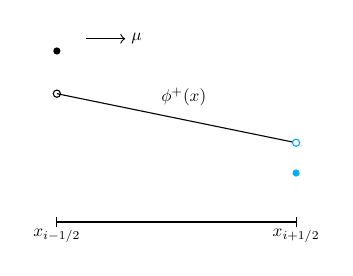
\begin{tikzpicture}[scale=0.62, every node/.style={transform shape}]
            \draw (1.0,4.0) node[fill,circle,inner sep=0pt,minimum
            size=4.2pt] {};
            \draw [->] (1.6,4.25) -- (2.4,4.25) node[anchor=west] {$\mu$};
            \draw (1.0,0.4) -- (1.0,0.6) node[below, pos=0.4] {$x_{i-1/2}$};
            \draw (5.90,0.4) -- (5.90,0.6) node[below, pos=0.4] {$x_{i+1/2}$};
            \node at (3.6,3.06) {$\phi^+(x)$};
            \draw [thick] (1.0,0.5) -- (5.9,0.5) node[anchor=north west] {};
            \filldraw[color=black, fill=white] (1,3.1250) circle (2.1pt);
            \draw (1.0,3.125) -- (5.90,2.120);
            \filldraw[color=cyan, fill=white] (5.9,2.120) circle (2.1pt);
            \draw (5.9,1.5) node[cyan,fill,circle,inner sep=0pt,minimum size=4.2pt] {};
        \end{tikzpicture}
    }}
    \caption{Linear doubly-discontinous representation for mean intensity in LO equations,
    for $\mu>0$.}
    \label{fig:ldd_space}
\end{figure}


\subsection{Issues with ECMC for Spatial Closure}
\label{sec:ecmc_issues}
There are several issues with ECMC that cause the LO moments to not exactly preserve
the HO moments, even for a linear problem.  With ECMC, global and, particularly, local
energy balance are generally not preserved.  For standard MC, there
are source biasing techniques (e.g., systematic
sampling) that exactly preserve the local zeroth moment of the
source and thus satisfy the local balance equations~\cite{shultis_mc,wollaber_review}). 
However, for our HOLO method, even with standard MC we have to reconstruct the bilnear moment
of $x$ and $\mu$, so the consistency terms lead to LO equations that do not exactly
preserve the first moment of the HO solution\footnote{It was verified that with
standard MC, systematic sampling, no analog sampling, and a closure that is only a
function of the zeroth moment, the LO solution exactly reproduces the HO moments, for
a linear problem}.  One final reason is that the analog treatment of absorption for
particles below the weight cutoff (e.g., see Sec.~\ref{sec:tallies}) results in
$\sigma_a \phi^{HO}_i$ and the amount of energy removed from a cell during MC
transport to not be equal; this is due to statistical noise in the path-length
estimators for $\phi^{HO}_i$.  However, ECMC will preserve balance to the order of
the iterative error and statistical noise, so the closure parameters will reproduce
the HO moments to the accuracy of the LO solution.  

\section{Test Problems}

To investigate the utility of the face closures we compare to the LD spatial
closure for two test problems.  We are interested in the accuracy of the solution and
consistency between the HO and LO solutions, particularly for coarser meshes. 
The consistency for the $(l)$-th particular simulation is measured with the relative L$_2$ norm
of the difference between the projected HO and LO solutions, i.e.,
\begin{equation}
    \|\phi_{HO} - \phi_{LO}\|^{(l)}_{2,rel} = \frac{\ds \sqrt{\int_0^X \left(
        \phi_{HO}^{(l)}(x) - \phi_{LO}^{(l)}(x) \right)^2 \dd x}}{\ds \sqrt{
            \int_0^X \left(\phi_{LO}^{(l)}(x)\right)^2 \dd x }}
\end{equation}
where $\phi_{LO}(x)$ and $\phi_{HO}(x)$ are the LDFE representations in space of the
intensity from the HO and LO solvers, from the end of the last time step.
The error between a reference solution and a fine solution for the ${(l)}$-th simulation
is computed as
\begin{equation}
    \|e\|^{{(l)}}_{2,rel} = \frac{\|\phi_{LO}^{n+1,{(l)}}(x) -
    \phi_{LO}^{n+1,ref}\|}{\|\phi_{LO}^{n+1,ref}\|}
\end{equation}
All L$_2$ norms are computed using quadrature over the finest spatial mesh.  An
integrated measure of the error in cell-averaged mean intensities on the mesh of the
$l$-th simulation, with $N_c^{(l)}$ spatial cells, is computed as
\begin{equation}
    \|e\|^{{(l)}}_{a,rel} = \left({\frac{\ds \sum\limits_{i=1}^{N^{(l)}_c}
    \left(\phi_i^{n+1,{(l)}} - \phi_i^{n+1,ref}
\right)^2}{\ds \sum\limits_{i=1}^{N^{(l)}_c}\left(\phi_i^{n+1,ref}\right)^2}}\right)^{1/2},
\end{equation}
where $\phi_i^{n+1,ref}$ is computed by spatially averaging the fine mesh solution over
the $i$-th coarse spatial cell.

The sample mean of each of the above metrics is estimated based on 20 independent
simulations; the sample standard deviation for each \emph{mean} is also reported, e.g.,
\begin{equation}
    s\left(\|e\|_{2,rel}\right) = \left[\frac{1}{20-1}\sum_{l=1}^{20} \left(
    \|e\|_{2,rel}^{(l)} - \|e\|_{2,rel} \right)^2\right]^{1/2},
\end{equation}
where $\|e\|_{2,rel}=\sum_{l=1}^{20}\|e\|_{2,rel}^{(l)}/20$ is the mean.

\subsection{Smooth Problem}

For this problem, the radiation and material energies are initially in
equilibrium at $0.01$ keV.   An isotropic incident intensity of 50 eV is applied
at $x=0$; the incident intensity on the right boundary is $10$ eV.
The material properties are $\rho = 1$ g cm$^{-3}$, $c_v = 0.2$ jks/keV-g, and
$\sigma_a=10$ cm$^{-1}$.
The simulation end time is 0.5 sh.  The time step size increases by 10\% each time step
until the maximum step size of 0.01 sh is reached, beginning from $\Delta t = 0.001$ sh.
This problem is intended to have less steep gradients in the intensity by having constant constant cross
sections, a smaller boundary source, and diffusive problem parameters.
The problem has a smaller optical thickness than other problems tested so that the face-based solutions can be efficiently
estimated, but the small c$_v$ value makes the solution relatively diffusive.  This
problem did not require the lumped relation to produce positive solutions.
However, when projecting from a refined mesh back to the coarse mesh, it was
necessary to rotate the solution to be positive.

All simulations of this problem used 585,900 histories divided over 9 ECMC
batches;  beginning from 30,000 histories and $10$ $\mu$ cells, 30\% of cells were
adaptively refined every third batch, and the number of histories is increased to
keep the average number of histories per cell constant. 
We have have performed two outer HOLO iterations over each time step for all cases; it was
found that additional iterations did not increase consistency, because of the  magnitude
of statistical noise.  Relative convergence of HOLO iterations was below 10$^{-3}$
for two iterations for all cases.  
Fig.~\ref{fig:smooth_compare} compares cell-averaged radiation temperatures for various spatial closures at
coarse mesh sizes and a fine-mesh solution.  The HO spatial closures curve is for the
scaled-slope closure given by Eq.~\eqref{eq:cl_slope}.  There was visually
no difference in the results between the scaled-averaged, scaled-slope, or LD closure. A step closure in all cells
was inaccurate for this problem.

Table~\ref{tab:smooth} compares the different error metrics for different spatial
closures and numbers of cells.  The reference solution for all calculations was the average of 10 simulations with $N_c=500$ spatial
cells.  In all cases, the HO spatial closure produces higher accuracy in the L$_2$
norms and greater consistency between the solvers.  However, there is not an
improvement in accuracy of the cell-averaged intensities.  Neglecting noise, the LDFE representation can be third order
accurate for the $\|e\|_a$ norm and second-order accurate in the L$_2$ norm~\cite{morel_ldtrt}. 
The statistical noise induced in face tallies makes the
additional accuracy that the MC transport can use not greater than the benefit of
higher spatial integration by the MC transport.  It
is noted that, overall, there is very low statistical noise in each of these
solutions due to the ECMC method and relatively high number of histories; at lower
history counts, the small gains of the HO spatial closure will degrade and stability
becomes an issue.

\begin{figure}[H]
    \centering
    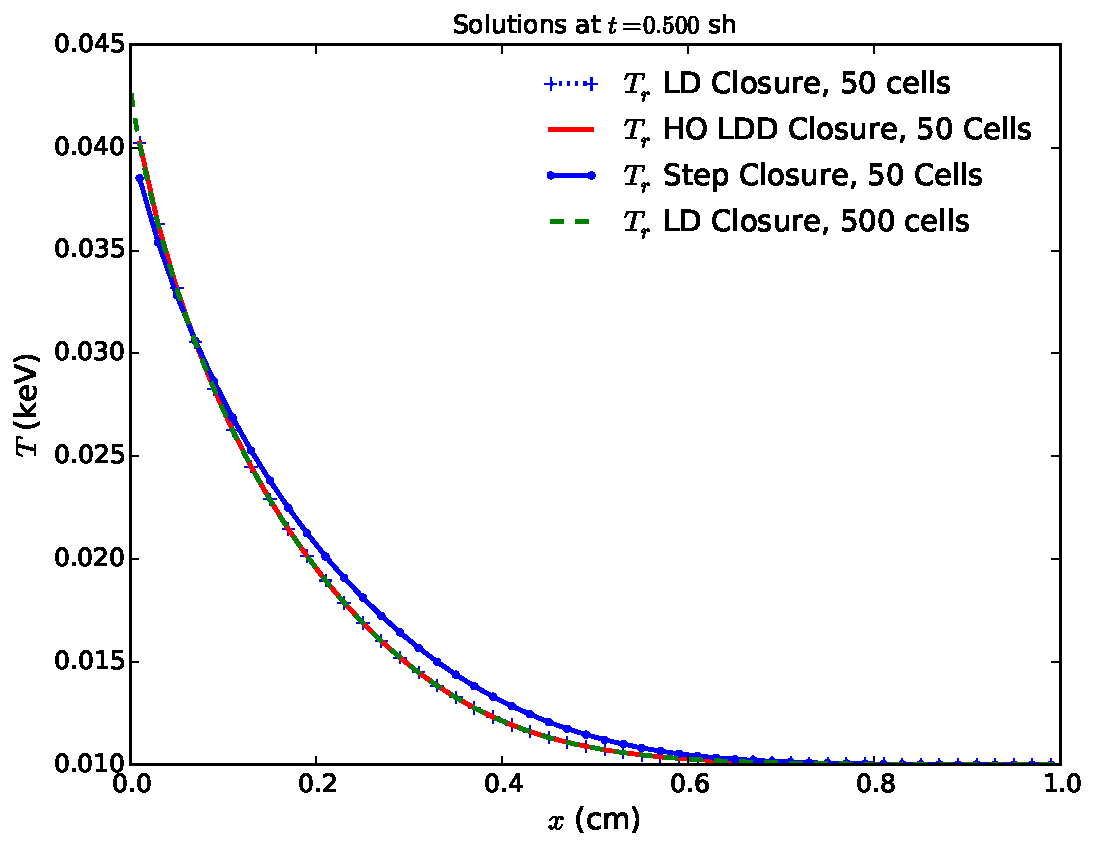
\includegraphics[width=0.99\linewidth]{smooth_compare.pdf}
    \caption{\label{fig:smooth_compare} Comparison of solutions for different spatial closures.}
\end{figure}

\begin{table}[H]
    \caption{\label{tab:smooth} Comparison of error metrics, reported as percentages, averaged over 20 simulations of smooth problem.  The absolute
standard deviation for each value is reported in parenthesis. Reference solution uses 500 cells.}
    \begin{tabular}{|l|cl|cl|cl|} \hline
        Spatial Closure & \multicolumn{2}{|c|}{$\|e\|_2$}  & \multicolumn{2}{|c|}{$\|e\|_{a}$} & \multicolumn{2}{|c|}{$\|\phi^{HO}
        -\phi^{LO}\|_{2}$} \\  \hline \hline
        \multicolumn{7}{|c|}{$N_c = 20$ cells} \\ \hline
LDFE               &   6.60\%  &   (0.17\%)  &   2.80\%     &   (5.7e-03\%)  &   2.90\%   &  (8.1e-03\%)  \\
HO: Scaled Slope   &   6.10\%  &   (2.9e-03\%)  &   3.50\%  &   (5.8e-03\%)  &   0.021\%  &  (8.6e-03\%)  \\
HO: Scaled Average &   6.10\%  &   (2.7e-03\%)  &   3.50\%  &   (5.0e-03\%)  &   0.023\%  &  (1.1e-02\%)  \\ \hline
       \multicolumn{7}{|c|}{$N_c  = 50$ cells}   \\ \hline
LDFE               &   1.60\%  &   (7.9e-04\%)  &   0.59\%  &   (3.8e-03\%)  &   0.76\%)  &  (4.8e-03\%)  \\
HO: Scaled Slope   &   1.40\%  &   (1.5e-03\%)  &   0.67\%  &   (3.2e-03\%)  &   0.012\%  &  (4.0e-03\%)  \\
HO: Scaled Average &   1.40\%  &   (1.5e-3\% ) &   0.67\%   &   (3.1e-03\%)  &   0.013\%  &  (3.9e-03\%)  \\ \hline
       \multicolumn{7}{|c|}{$N_c  = 100$ cells}   \\ \hline
LDFE               &   0.53\%  &   (2.1e-03\%)  &   0.15\%  &   (2.5e-03\%)  &   0.30\%)  &  (9.7e-03\%)  \%\\
HO: Scaled Slope   &   0.45\%  &   (1.5e-03\%)  &   0.16\%  &   (4.6e-03\%)  &   0.012\%  &  (4.8e-03\%)  \\
HO: Scaled Average &   0.45\%  &   (1.4e-03\%)  &   0.16\%  &   (4.7e-03\%)  &   0.012\%  &  (3.6e-03\%)  \\ \hline
    \end{tabular}
\end{table}



\section{Two Material Problem}

The HO spatial closures were applied to solution of the two material problem detailed in Sec.~\ref{sec:two}.
For these results, the time step size is increased from 0.001 sh to a maximum step of 0.01 sh by 5\% each
step, with the final step adjusted to end at 2 sh.

The scaled-slope closure was found to not stably converge, even for 3 batches of 10$^6$
histories.  This coudl be caused the steep gradients at the foot of the wave.  As the
solution slightly overshoots, the slope changes signs between cells. 



\chapter{Results}


\section{Preservation of the Discrete Maximum Principle}

An important property of a discretization of the TRT equations is preservation of the
discrete maximum principle (MP).  Violation of the maximum principle results in
the material temperature being artificially higher than the boundary conditions and
sources should physically allow. As discussed in Sec.~\ref{sec:intro}, IMC can violate the MP due to the approximate
linearization of the emission source in the time discretization; it is not truly implicit in time. 
We expect our
method, with a truly implicit time discretization, to preserve the MP with sufficient
convergence of the nonlinear emission source~\cite{larsen_mpv}.

To numerically demonstrate that our method preserves the MP, we have simulated problems similar to those in~\cite{wollaber2013discrete}.
We modify the Marshak wave problem in Sec.~\ref{sec:marshak???} to produce a problem which
results in MP violations for IMC at various time step sizes.  The material specifications
are given in Table~\ref{tab:mpv_prob}. The domain width is 1.0 cm wih $N_c=150$ spatial mesh cells.  The radiation and material energies are initially in
equilibrium at $0.01$ keV, before an isotropic boundary source of $1$ keV is applied at
the left boundary at $t=0$. The simulation is ran unitl $t=0.1$ sh. 

The material and radiation temperature are given for an IMC simulation in Figure~\ref{fig:imc_mpv1}.  Figure~\ref{fig:imc_mpv} depicts the material temperature for various time step sizes and a ifxed
mesh size of 150 equally spaced cells. All IMC simulations used 100,000 histories. As demonstrated, the material temperature exceeds the boundary condition and is artificially hotter than the radiation temperature.  As larger timestep sizes are taken the nonphysical results worsen.  This is a clear violation of the MP.

The simulations are repeated with the same specifications





The spatial and temporal discretization affects the appearance of MP violations for
IMC~\cite{wollaber2013discrete}. In particular, if time steps are too large or spatial
mesh cells are too small, IMC will demonstrate MP violations.  Here, we have kept the
spatial mesh size fixed and increased time step to make MP violations appear.

8 $\mu$ cells, 3 batches of 6,000 particles each.

The radiation boundary source temperature is at $1$ keV. The fact that the material
has exceeded teh boundary condition is referred to as a MP violation.


The damped newton is necessary.

NO FIXUP APPLIED, NEWTON CONVERGENCE OF 10e-06.  MODIFIED MARSHAK WAVE PROBLEM.

ACCURACY ALSO AN ISSUE.  even for short time step at early time steps it does appear

\begin{table}[H]
        \caption{\label{tab:mpv_prob}Problem specifications for maximum principle
        violation. Absorption cross section has form $\sigma_a = \sigma_{a,0}/T^3$.}
\centering
        \begin{tabular}{|c|c|} \hline \\
            $\sigma_{a,0}$ (cm$^-1$ keV$^3$)  & 4.0  \\
            $\sigma_s$ (cm$^{-1}$) & 0.0 \\
            $\rho$ (g cm$^-3$) & 1.0  \\
            $c_v$ (jks/keV-g) & 0.0081181  \\ 
        \end{tabular}
\end{table}



   An isotropic incident intensity of 0.150 keV is applied
at $x=0$; the incident intensity on the right boundary is $2.5\times10^{-5}$ keV.
The material properties are $\rho = 1$ g cm$^{-3}$ and $c_v = 0.013784$ jks/keV-g. The
absorption cross section varies as $\sigma(T) = 0.001\;\rho\; T^{-3}$ (cm$^{-1}$).
The simulation was advanced until $t=5$~sh~(1~sh~$\equiv$~10$^{-8}$~s) with a fixed time step size of 0.001 sh. For comparison purposes, we
have not used adaptive mesh
refinement, only performed one HOLO iteration per time
step, and use a fixed 3 HO batches with equal number of histories per batch. A
relative tolerance of $10^{-6}$ for the change in $\phi(x)$ and $T(x)$ was used for
the LO newton solver for all results. Radiation energy
distributions are plotted as an equivalent temperature given by
$T_r=(\phi/(ac))^{0.25}$.  Cell-averaged quantities are plotted.
Although isotropic scattering can be included in the LO solver with this method~\cite{ans_2014}, we have only
considered problems with $\sigma_s = 0$ here.  


%
\setlength{\baselineskip}{12pt}
\clearpage
\bibliographystyle{plain}
\bibliography{references}
\clearpage


\end{document}
